\documentclass[master]{thesis-uestc}

\title{基于信息融合的目标聚集\\预测算法研究}{Research on Target Gather Prediction Algorithm based on Information Fusion}

\author{}{}
\advisor{}{}
\school{计算机科学与工程学院}{School of Computer Science and Engineering}
\major{计算机科学与技术}{Computer Science and Technology}
\studentnumber{}

\begin{document}
\makecover
\begin{chineseabstract}
聚集预测是对城市中可能存在的人群聚集现象进行预测,能够帮助政府更好的应对城市中的聚集问题,增强各部门的应对能力,大幅提升城市治理水平。城市场景下生活规律性强,道路结构复杂,地理环境、假期、天气等因素对用户行为模式影响较大。且多目标交互复杂,需要同时考虑行人、车辆、公共交通等。现有方法存在对外部知识考虑不足、多用户关联关系刻画不准的问题,导致模型预测精度不高。

基于上述问题,本文围绕基于信息融合的目标聚集预测算法开展研究,具体研究内容如下:

1、提出了基于时空门控循环单元(STGRU)的轨迹预测模型。现有的算法模型忽略了地理环境信息、假期信息、天气信息等外部知识对运动模式的影响。为此,本文提出了融合路网门控结构,实现了对以路网结构为代表的地理环境特征提取和外部知识的融合,从而实现更准确的用户行为模式建模,并在一定程度上减少模型参数量。通过实验表明,考虑路网结构和外部知识可以有效提高轨迹预测性能,相较于现有方法的性能提升最高可达18.1$\%$。

2、提出基于空间特征增强的的聚集预测模型。当前的时空特征挖掘算法不能同时建模多用户之间关联特征,本文提出了基于希尔伯特曲线与图嵌入的空间特征增强方法,通过使用希尔伯特曲线进行标签设计增强了标签间的空间关系,同时通过融合图嵌入方法实现了多用户场景下的实时路网结构特征提取。通过实验表明,能够有效提升模型对多用户时空特征的建模能力,性能提升幅度最高为22.6$\%$。

3、完成基于城市流量的聚集预测告警系统。为了验证算法的实用性,结合实际需求,设计并实现了基于城市流量的聚集预测告警系统,实现了城市级别的多目标聚集预测,为城市的管理管控提供有利支撑。

\chinesekeyword{聚集预测,复杂场景,智慧城市,深度学习,时空特征挖掘}
\end{chineseabstract}

\begin{englishabstract}
Gather prediction is to predict the possible crowd gathering phenomenon in the city. Gather prediction can help the government deal with the gathering problems, and enhance the coping ability of various departments. Gather prediction can significantly improve the level of urban governance. The urban scene has a strong regularity of life, complex road structure, and factors such as geography, holidays, and weather have a large impact on user behavior patterns. And the multi-objective interaction is complex, and pedestrians, vehicles and public transportation need to be considered simultaneously. The existing methods have the problems of insufficient consideration of external knowledge and inaccurate portrayal of multi-user association relationships, which lead to low model prediction accuracy.

Based on the above-mentioned problems, this paper conducts research around the target gather prediction algorithm based on information fusion as follows.

1.Thesis proposes a trajectory prediction model based on spatio-temporal gated recurrent unit (STGRU). The existing trajectory prediction algorithms ignore external knowledge such as geographic environment, holiday and weather information affects the movement patterns. To this end, a fused road network gating structure is proposed to achieve the fusion of geographic environment feature extraction and external knowledges, so as to achieve more accurate user behavior pattern modeling and reduce the number of model parameters. It is shown through experiments that considering the road network structure and external knowledge can effectively improve the trajectory prediction performance, and the performance improvement is up to 18.1$\%$ compared with the existing methods.

2.Thesis proposes a gather prediction model based on spatial feature enhancement.The spatial feature enhancement method based on Hilbert curves and graph embedding is proposed to address the problems of the existing spatio-temporal feature mining algorithms in label design and explicit feature extraction methods. The model enhances the spatial relationship between labels by using Hilbert curves for label design, and realizes real-time road network structure feature extraction in multi-user scenarios by fusing graph embedding methods. It is shown through experiments that the model can effectively improve the modeling ability of multi-user spatio-temporal features with the highest performance improvement of 22.6$\%$.

3. Complete the gather prediction alert system based on city flow. In order to verify the practicality of the algorithm, the gather prediction alert system based on city flow is designed and implemented in conjunction with the actual demand, which realizes the multi-objective gather prediction at the city level and provides favorable support for the management control of the city.

\englishkeyword{gather prediction, complex scenario, smart city, deep learning, spatio-temporal feature mining}
\end{englishabstract}


\thesistableofcontents

\chapter{绪\hspace{6pt}论}

\section{研究工作的背景与意义}
随着城市中物联网设备的不断增加\citing{DBLP:journals/computers/SejdiuIA21}和5G\citing{DBLP:journals/adhoc/SharmaJGC21}等技术的普及,城市场景下能够获取到的轨迹数据呈爆发式增长。海量的轨迹数据\citing{DBLP:journals/complexity/ChaoHFWCLY21}为基于大数据技术的机器学习、深度学习发展提供了良好的数据支持,轨迹预测\citing{DBLP:journals/pr/0007PPF21}、聚集预测\citing{DBLP:conf/gistam/OsaragiH20,DBLP:journals/tsas/WangCCPH20}、交通流量预测\citing{DBLP:journals/eswa/LiuQ21}、热点区域分析\citing{DBLP:books/sp/21/PretoMAMM21}、人口转移预测\citing{DBLP:conf/cec/LiuW21}等研究方向受到了越来越多研究者的关注,其中聚集预测受到了越来越多城市管理者的重视。近年来由人群聚集所带来的问题对城市管理影响重大。首先是新型冠状病毒在全球的传播和蔓延\citing{DBLP:journals/ijon/AlassafiJA22},新冠疫情的传播和暴发很大程度上依赖于人群聚集。如今我国已经能够较好的控制新型冠状病毒疫情的传播,但仍需时刻保持警惕,避免聚集的发生,特别是节假日或大型活动的举办。其次,人群聚集极为容易发生踩踏伤人等事故,以及某些恶性事件\citing{DBLP:journals/bigdatama/SreenivasuluS20}的发生,需要及时进行疏散。

当前聚集预测算法通常对用户轨迹预测结果进行融合得到聚集预测结果,不能很好地提取用户关联特征\citing{DBLP:journals/wc/WuISW21},在多轨迹任务\citing{DBLP:journals/jmlr/LuMT21}上仍存在较大局限性。一方面,现有的模型在提取时空特征时未考虑地理环境信息\citing{DBLP:conf/kdd/LianWG0C20}、假期信息、天气信息等外部知识\citing{DBLP:conf/kdd/YuanZXS11}的影响。另一方面,当前方法在对用户轨迹进行预测时主要针对单一轨迹进行设计,建模单用户的行为模式\citing{DBLP:conf/kdd/LianZXSCR14,DBLP:conf/sigir/LiCLPK15,DBLP:conf/ijcai/ChengYLK13,DBLP:conf/aaai/LiuWWT16},并未考虑用户关联特征。

为此,本文围绕基于时空轨迹预测的聚集预测算法进行研究,首先设计结合路网结构的时空门控网络,通过提取路网结构特征和融合多种外部知识的方法,提升了对时空特征的建模能力。其次通过空间特征增强方法,提取用户之间的关联特征,提升模型在多用户场景下的行为模式建模能力。并在多个数据集上设置和进行了多项实验,验证了模型的可行性和预测性能。

本文的研究能够根据城市中的用户分布情况以及采集的用户历史轨迹信息对每个用户的位置进行预测,对每个用户的位置预测结果通过统计的方法得到用户之间的聚集情况,聚集预测结果可以帮助城市管理部门提前做出反应,并大大减少恶性聚集造成的损失和风险。

\section{国内外研究历史与现状}
聚集预测是时空数据分析\citing{刘大有2013时空数据挖掘研究进展}和挖掘中\citing{DBLP:conf/ijcai/WuLJC19}的重要组成部分,它包括很多应用场景,如热点区域分析、客流预测\citing{DBLP:journals/eaai/JinSLZ22}、人口转移预测等。Tomaharu等人\citing{DBLP:conf/aaai/IwataS19a}提出了一个集体图模型来预测区域间的转移人口,Verma等人\citing{verma2017pam}利用轨迹数据挖掘热点,实现了非实时的粗粒度聚集预测。Ni等人\citing{DBLP:journals/tits/NiHG17}通过客流预测实现了城市间的聚集预测。Kumar等人\citing{DBLP:journals/vc/KumarBRLP17}利用轨迹聚类\citing{DBLP:conf/kdd/LianZXSCR14,DBLP:conf/sigir/YeYLL11}和相似性分析进行聚集预测。聚集预测也可以转化为同一时间和空间下的多轨迹预测任务,即关注多个轨迹之间的时间和空间特征。时空数据的数据挖掘\citing{DBLP:journals/air/HamdiSEMRS22}非常困难,也是目前的研究热点之一。

本节先介绍以马尔可夫链为主的传统位置预测算法,再对基于神经网络模型的位置预测方法进行阐述,最后对现有工作进行总结。

\subsection{传统位置预测方法}
位置预测的主要特征是地理信息和时间信息。位置预测还可以使用位置语义\citing{DBLP:conf/aaai/GuoSZT20}、速度、方向。在传统概率的基础上,矩阵分解法用低秩矩阵去组合矩阵,得到用户和轨迹的隐含特征向量。张量分解法扩展到三个维度,包括用户、时间信息和空间信息。

经典基于序列数据的预测模型通常采用马尔可夫链模型\citing{DBLP:conf/eurocast/Moreno-DiazVMI03}。马尔可夫链(Markov Chain,MC),具有离散时间的特性,可以表示为状态空间中多个状态之间转换的随机过程,且该过程具有独立性,即任一状态的概率分布只取决去前一个状态。根据下一时刻状态由当前时刻和前$m-1$个时刻决定,称为$m$阶马尔科夫链。基本马尔科夫链模型基于转移矩阵,通过上一时刻的状态来预测下一时刻的状态,比较适合建模个人的序列。但是比较容易受到最近的噪声影响\citing{DBLP:journals/jair/BegleiterEY04}。

在MC的基础上,FPMC\citing{DBLP:conf/www/RendleFS10}对每个用户建模了一个马尔可夫转移矩阵,组成了一个转移张量,来融合序列和个性化两个方面的信息,称为个性化马尔可夫链,通过成对交互的张量分解来解决数据稀疏的问题。对用户、当前状态、下一时刻状态之间的成对关系设置两方面的嵌入表示,通过点积的和来估算,降低了计算复杂度且参数量更少,同时显示建模成对的交互关系更为直接。但是FPMC中将每一个状态进行了两次嵌入,在轨迹预测中,将两个状态嵌入到两个相互独立的空间中是不恰当的,不能很好的捕捉两者转化的关系,FPMC存在一些变种模型\citing{DBLP:conf/ijcai/ChengYLK13},但都没有从根本上解决这个问题。

根据位置预测任务在FPMC的基础上进行了改进,提出了PRME模型\citing{DBLP:conf/ijcai/FengLZCCY15},将状态统一嵌入到一个欧式的度量空间中,使用向量间的欧式距离作为相似度的衡量方式。后续还有一部分基于图嵌入\citing{DBLP:conf/cikm/XieYWXCW16}的工作,将其扩展到非欧式空间中。

\subsection{基于神经网络模型的位置预测方法}
随着近几年机器学习和深度学习的发展,部分任务需要处理序列数据,循环神经网络在序列处理上取得了巨大的提升,成为时间序列预测最好的方法。RNN以及其变种模型LSTM、GRU的发展,使得神经网络模型在序列预测任务上保持最好的效果。

之后的模型发展更专注于对时空特征的建模,更多考虑轨迹的上下文信息\citing{DBLP:journals/tkde/SongXWWZZ017,DBLP:conf/cikm/SordoniBVLSN15}和轨迹点之间间隔距离等信息,基于基础模型发展出了STF-RNN、ST-RNN、HST-LSTM、STGN等一系列效果更好或更符合实际情况的模型。

\subsubsection{基于时间序列的神经网络模型}
随着神经网络领域研究的深入,神经网络模型在大多数任务上取得了较好的效果。最传统的神经网络模型是前馈神经网络,通过层与层之间的全连接对数据进行拟合,这样的结构也导致了传统的神经网络模型对很多问题是无法解决的,最典型的就是序列数据。神经网络的优势在于能够对多维度信息之间的非线性关系进行建模,广泛应用于推荐领域\citing{DBLP:conf/mm/WangW14,DBLP:conf/kdd/ZhangYLXM16,DBLP:conf/www/HeLZNHC17,DBLP:journals/ijon/CuiWHW19}。

为了能够处理序列数据又能拥有神经网络模型的建模能力,Wojciech等人提出了循环神经网络(Recurrent neural network,RNN)\citing{DBLP:conf/interspeech/MikolovKBCK10}。RNN与前馈神经网络的区别在于对历史信息的记忆和计算。通过连接隐藏层中的相邻节点构建了重复模块链,借助上一时刻的输出计算当前状态。RNN在位置预测任务上,一度是效果最好的模型。

但由于RNN本身结构的限制,为了适应现有的使用现状,一般都仅考虑当前状态只与前面的几个状态相关,这与马尔科夫链模型的本质上十分相近,仅是借助于神经网络强大的建模能力,但是RNN并未考虑到反向传播时的累乘问题,存在严重的梯度消失和梯度爆炸问题。

现实场景中序列数据的状态取决于其上下文状态以及较远的历史状态,而RNN对于历史状态并不能很好的建模。长短时记忆网络(Long Short-term Memory,LSTM)\citing{DBLP:journals/neco/HochreiterS97}通过结构优化实现了对长间隔事件的处理和预测。LSTM相较于RNN最大的进步在于对长期依赖性的建模,长时间记住信息实际上是LSTM的默认行为,LSTM精心设计了门控结构来选择性的添加或移除信息,同时大幅缓解了梯度爆炸和梯度消失问题。

门控循环单元(Gate Recurrent Unit,GRU)\citing{DBLP:conf/emnlp/ChoMGBBSB14}是一种LSTM优化模型。GRU在保留了LSTM结构的优点的前提下对结构进行了精简,较LSTM减少了一个门控,参数比LSTM少,更便于计算和训练。

LSTM和GRU是目前通用序列数据处理建模最为先进的范式模型,但对于位置预测任务来说,还有很多不足之处能够进一步改进。例如LSTM并不能建模轨迹数据中的空间关系。

\subsubsection{建模时空特征的神经网络模型}
这部分工作是在RNN和LSTM的基础上增加了空间依赖性建模\citing{DBLP:conf/aaai/SunQCLNY20}的方式,更适合用于位置预测等数据间存在强烈空间关系的任务。

针对RNN难以建模时间间隔信息以及位置之间的地理距离的问题,Liu等人\citing{DBLP:conf/aaai/LiuWWT16}提出了时空循环神经网络STRNN,分别设计了特定时间间隔的过渡矩阵和地理距离的过渡矩阵。在一定程度上对轨迹的时空信息进行了建模,但是较为生硬,特征之间不能很好的融合,且STRNN中的时空特征提取需要经过手工处理。基于时空特征循环神经网络STF-RNN\citing{DBLP:conf/ssci/Al-MolegiJG16}能够自动提取空间和时间特征内部表示,而不是依靠手工表示。这使模型能够更有效地发现有关人的行为的有用知识,保留了RNN结构来建模用户移动历史。相较于ST-RNN中过渡矩阵的方法,STF-RNN能够根据数据本身特点学习到不同的时间和空间特征。

Geo主题模型\citing{DBLP:conf/wsdm/KurashimaIHTF13}采样基于主体和用户与历史位置之间的距离。GMEL模型\citing{DBLP:conf/aaai/Liu0XYWS20}结合位置语义来嵌入地理环境信息。上述研究表明,连续轨迹点之间的顺序在位置预测中起着至关重要的作用,在强实时轨迹数据场景下效果更为显著,因为人类行为模式\citing{DBLP:conf/www/FengLZSMGJ18,DBLP:conf/wsdm/TangW18}是有顺序的。

ST-LSTM模型\citing{DBLP:conf/ijcai/Kong018}同时考虑轨迹点之间的时间间隔和距离间隔,通过将时间间隔和地理距离划分为离散时隙并仅对这些时隙的上限和下限进行编码来解决间隔的稀疏性问题,将其单独进行建模并添加到经典LSTM模型的每个门控中。相当于在原始输入的基础上添加了时间和距离的手工处理,但是并没有使用单独的门控结构进行显式的特征提取。STGN模型\citing{DBLP:conf/aaai/ZhaoZLXLZSZ19}通过在LSTM中引入时空门控以捕获连续轨迹点之间的时空关系,设计了两对时间门控和距离门控,对时间间隔和距离间隔单独进行建模,而不是像ST-LSTM直接添加到输入门、输出门、遗忘门之中,能够对时间和距离更好地建模。STGN是目前效果最好的模型,但同样存在一定的问题,过多的考虑相邻轨迹点之间的时间间隔和地理距离,并不能很好的与LSTM本质上长期记忆的轨迹点与当前轨迹点之间的关系,对时空关系的建模并不完善,且额外对当前轨迹点的建模进行差异的记忆处理,导致参数量成倍的增加。

\subsection{现有工作总结}
在位置预测相关领域中,传统方法通过求解状态空间中的转移概率对数据进行建模,建模能力较弱且对位置预测任务中至关重要的语义特征难以融合。同时传统方法对噪声较为敏感,因此数据质量要求很高,不适用于大多数实际应用场景。

基于神经网络的方法能够凭借其技术特点大幅提升对时空数据的建模能力,但通用的基于时间序列的神经网络模型在时空特征建模时受到了较大的限制,难以建模数据中的空间特征。

建模时空特征的神经网络模型在时间序列神经网络模型的基础上增加了对空间信息的建模,并增加了时空特征的权重得到更强的建模能力。目前这类方法已经能够实现时空特征的自动提取,并解决了固有的短期记忆问题,但带来了模型参数量的成倍增长。同时现有的方法中仅通过各点间距离信息建模空间特征,忽视了固有地理环境及其状态的影响。

\section{本文的主要贡献与创新}
聚集预测任务的主要研究难点在于对轨迹数据中时空特征的建模以及多用户之间关联特征的建模。时空特征建模主要通过扩展各类时间序列神经网络实现。然而目前的各类方法均忽略了路网等地理环境信息以及天气信息、假期信息等外部知识对用户行为模式的影响,且为了对时空特征进行建模导致参数量的成倍增长。关联特征建模

针对上述问题,本文主要研究模型在聚集预测场景下的时空特征提取建模能力,主要创新点与贡献如下:

1、针对现有的算法模型忽略了地理环境信息、假期信息、天气信息等外部知识对运动模式的影响问题,本文提出了时空门控循环单元(Spatio-Temporal Gated Recurrent Unit,STGRU),实现了对以路网结构为代表的地理环境特征提取和外部知识的融合,从而实现更准确的用户行为模式建模,并在一定程度上减少模型参数量。通过实验表明,考虑路网结构和外部知识可以有效提高轨迹预测性能,相较于现有方法的性能提升最高可达18.1$\%$。

2、针对当前的时空特征挖掘算法不能同时建模多用户之间关联特征的问题,本文提出了基于空间特征增强的的聚集预测模型(Spatial Enhanced Gather Prediction Model,SEGPM),通过使用希尔伯特曲线进行标签设计增强了标签间的空间关系,同时通过融合图嵌入方法实现了多用户场景下的实时路网结构特征提取。通过实验表明,能够有效提升模型对多用户时空特征的建模能力,性能提升幅度最高为22.6$\%$。

3、完成基于城市流量的聚集预测告警系统。为了验证算法的实用性,结合实际需求,设计并实现了基于城市流量的聚集预测告警系统,实现了城市级别的多目标聚集预测,为城市的管理管控提供有利支撑。

\section{本论文的结构安排}
本文的后续章节结构安排如下:

第二章,相关理论基础。首先介绍了本文中涉及的各类深度学习算法模型的基础知识,再介绍了近年来的时空特征建模相关算法,最后介绍了本文对数据集的选择及所使用的轨迹数据集的整体情况。

第三章,基于时空特征的轨迹预测方法。首先根据当前轨迹预测方法存在的问题提出解决思路。然后详细介绍了本文中所提出的时空门控循环单元(STGRU)的结构与原理。最后,通过实验验证所提出模型建模时空特征的有效性。

第四章,基于希尔伯特曲线与图嵌入的空间特征增强方法研究。首先分析轨迹预测方法在聚集预测任务下的局限性,并详细介绍了希尔伯特曲线和图卷积算法的原理。然后详细阐述了增强轨迹数据空间特征的聚集预测模型。最后,并通过实验验证该方法对于聚集预测的有效性。

第五章,基于城市流量的聚集预测告警系统实现。结合本文研究内容和实际场景,设计并实现了一个聚集预测告警系统。并从需求分析、功能设计实现并通过可视化demo对系统进行展示。

第六章,总结与展望。对本文所做的工作及存在的缺点进行了总结,并构思了后续的研究可能。

\chapter{相关理论基础}
本章主要介绍后文中所用到的序列神经网络相关理论基础以及三种基于深度学习的时空特征建模方法,并对本文所使用的数据集进行了介绍。

\section{引言}
时空数据是人类活动中产生和采集到的最多的数据,从时空数据中发现知识对于解决现实世界中的诸多问题有很大的意义。随着深度学习算法的发展,越来越多的研究者开始关注基于时空数据的应用和挖掘。其中,最核心的问题就是如何对时空特征进行建模分析,近年来在不同应用领域都针对该问题开展了研究。

本章首先介绍本文提出模型所涉及的序列神经网络相关理论基础,然后阐述了时空特征建模方法的发展,最后对本文中所有使用的数据集进行分析。

\section{相关技术}
本文所涉及的相关技术面较广,为了方便理解,本节对本文所提出模型相关的技术要点进行详细介绍。

\subsection{循环神经网络}
2012年,AlexNet模型\citing{DBLP:conf/nips/KrizhevskySH12}在计算机视觉领域首次达到了人类的精度,之后随着各领域数据的增加极大的推动了深度学习与神经网络的发展。其中,序列数据的建模在各领域都得到了广泛的研究。

时间序列数据\citing{DBLP:journals/bigdata/TorresHSMT21}是指拥有不同时间戳的数据,根据时间的天然连续性这类数据能够反映出事物或现象随时间变化的过程。前馈神经网络\citing{rosenblatt1958perceptron}会给每个输入维度分配一个单独的参数,在每个时间点都是一个单独的参数,对于变长序列泛化能力极差,且难以实现不同位置的参数共享。循环神经网络(RNN)通过设计循环计算结构实现了不同方式的参数共享,能够适用于各类序列数据的建模,并成为了应用最广泛的神经网络模型之一。

\begin{figure*}[!ht]
\centering 
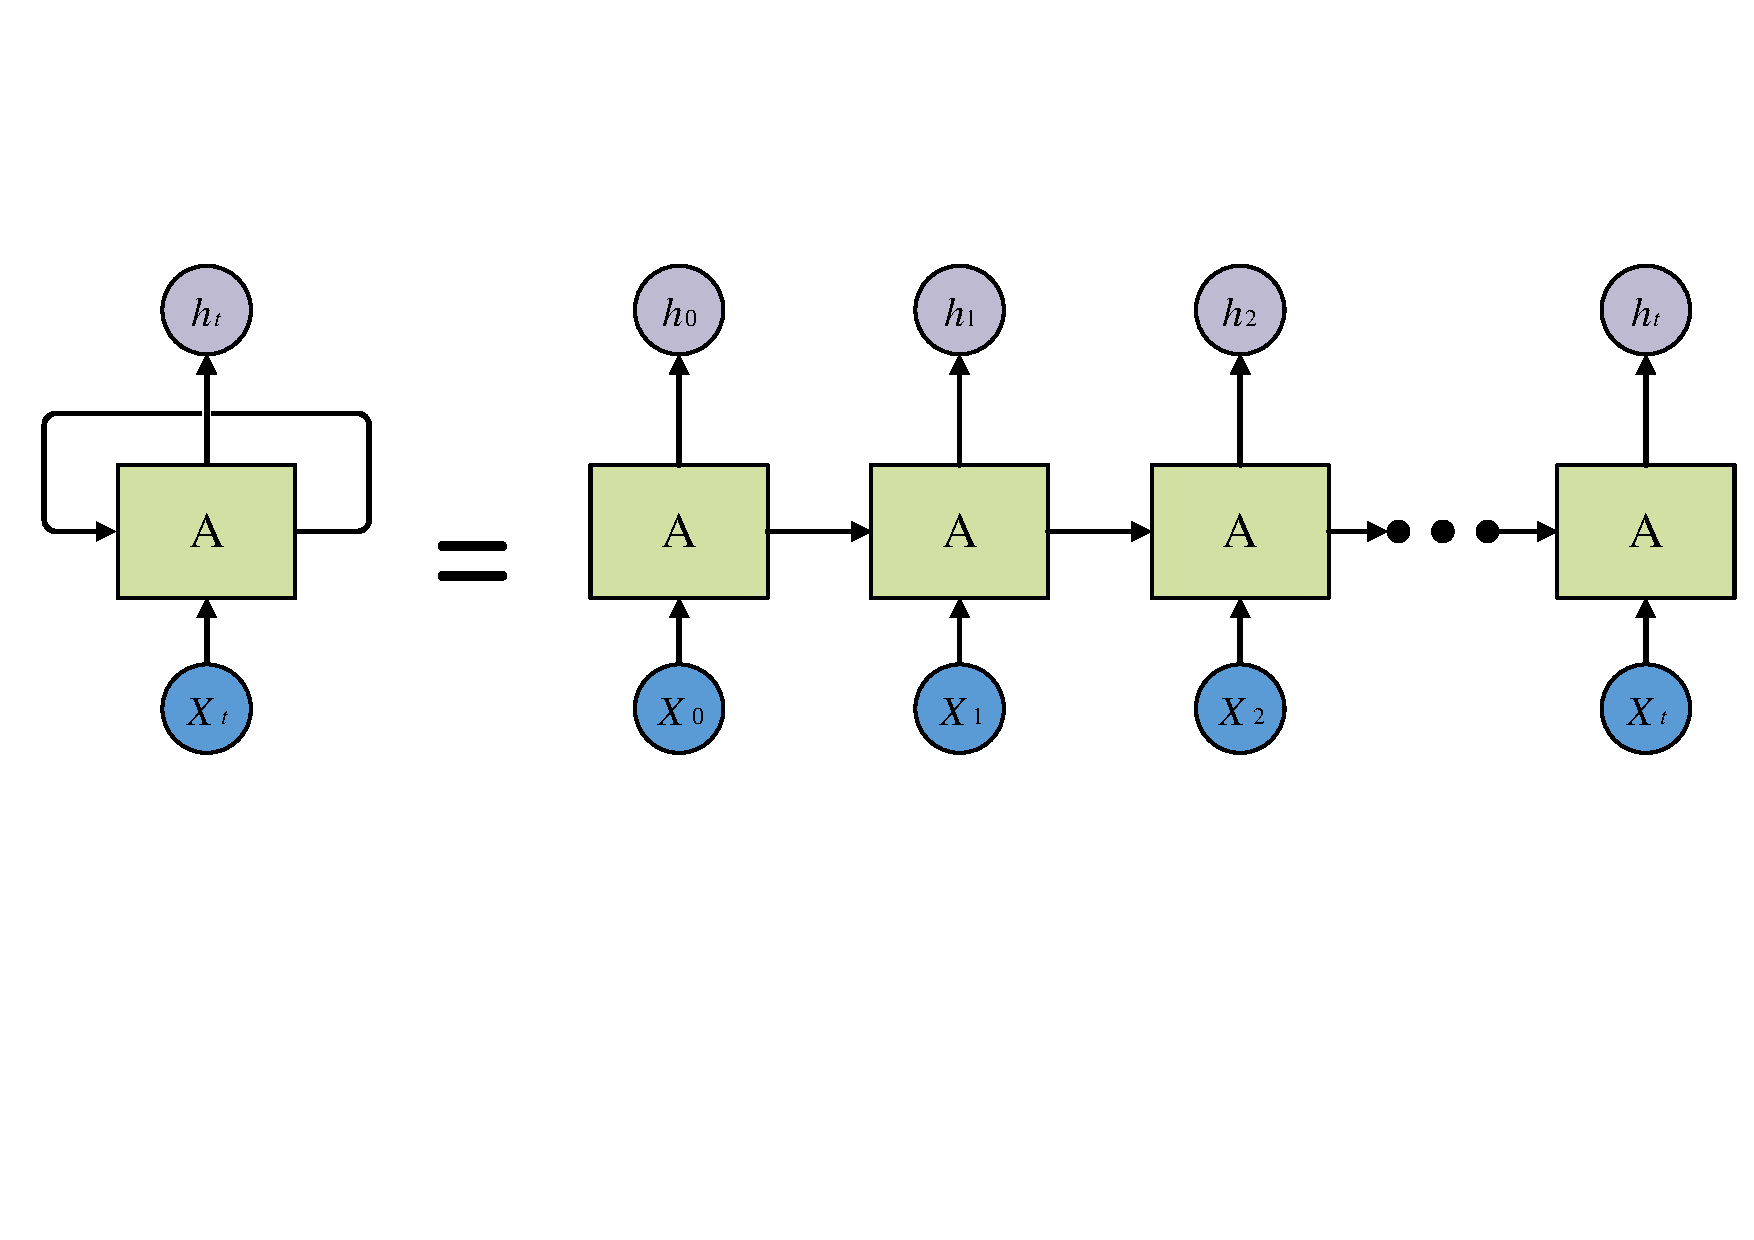
\includegraphics[width=0.7\textwidth]{./pic/RNN-2.pdf}
\caption{循环神经网络RNN}
\label{Figure.2.1}
\end{figure*}
如图\ref{Figure.2.1}所示为RNN的网络结构,由输入层、隐藏层和输出层构成。其中最基本的单层网络结构的定义为输入$x$,经过变换和激活函数$f$得到输出$y$:
\begin{equation}
   y = f(x;\theta)
\end{equation}

而对于序列数据$(x_1,x_2,\dots,x_n)$,在$t$时刻时所包含向量为$x^{(t)}$。为了能够实现不同时间步之间能够进行循环计算,RNN引入了隐藏状态$h$的概念:将前一次的输出结果作为下一次的输入一起训练。
\begin{equation}
   h^{(t)} = f(h^{(t-1)},x^{(t)};\theta)
\end{equation}

循环结构的引入使得循环神经网络能够对不同长度的序列都具有相同的输入大小,以及在每个时间步使用相同的参数,而不需要为每个时间步学习独立的模型。根据使用场景的不同,循环神经网络能够实现单一输入多输出、多输入单一输出、多输入多输出以及作为编解码器等多种方式.

\begin{figure*}[!ht]
\centering 
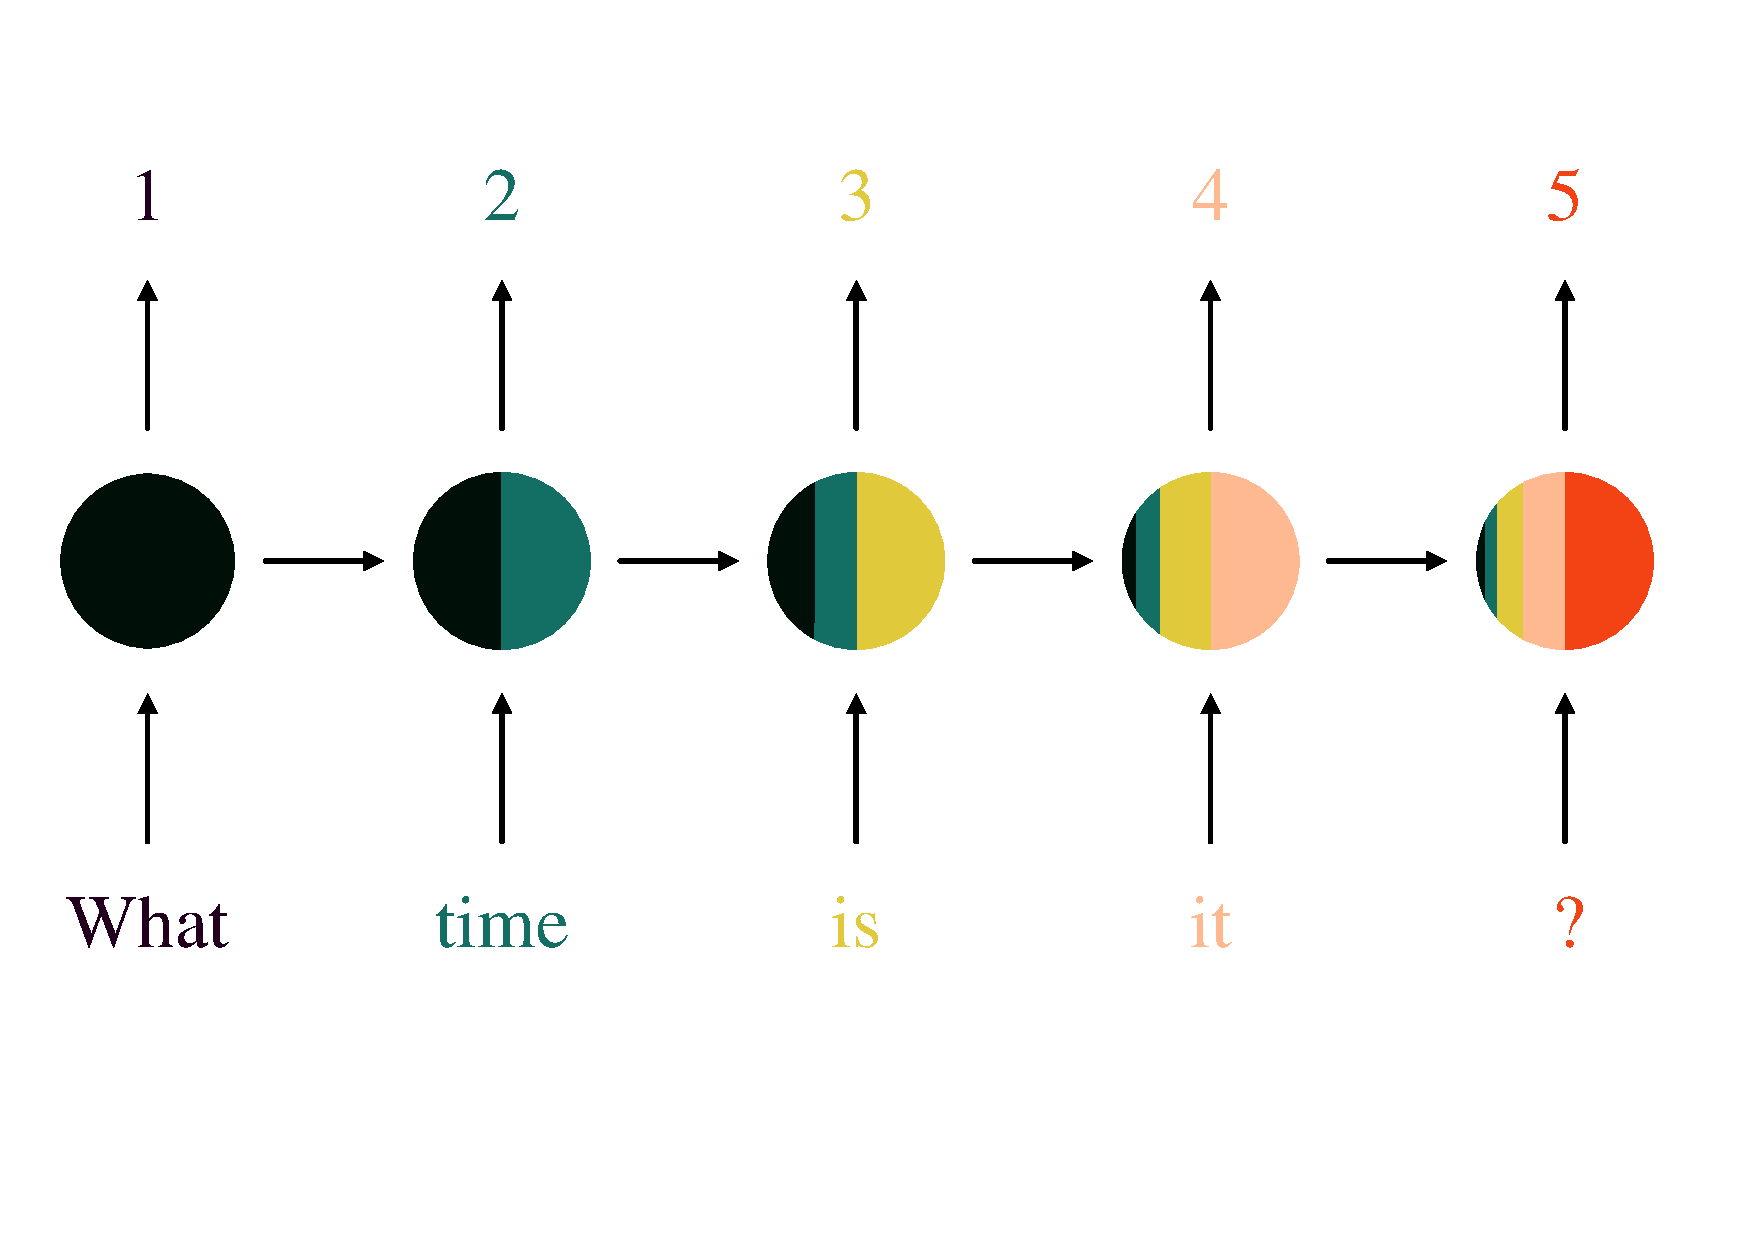
\includegraphics[width=0.7\textwidth]{./pic/rnn4.pdf}
\caption{循环神经网络的短期记忆问题}
\label{Figure.2.2}
\end{figure*}
然而RNN未能解决长期依赖的挑战,如图\ref{Figure.2.2}所示为RNN在文本预测任务中的应用,短期记忆对计算结果影响较大,长期依赖所占的权重比例很小,这也就导致了RNN存在短期记忆问题。同时在循环神经网络的训练过程中,随着序列长度的增加,取决于梯度的幅值,梯度会不可避免的趋向于0或者无穷,这就导致了梯度消失和梯度爆炸问题。

简单的通过限制参数空间是不能避免梯度消失和梯度爆炸问题的,为了能够表示长期依赖关系并使模型具有一定程度的鲁棒性,RNN必然会进入参数空间中的梯度消失区域\citing{DBLP:journals/tnn/BengioSF94}。

\subsection{长短时记忆网络}
长短时记忆网络(LSTM)是一种特殊的循环神经网络,最早由
Hochreiter等人\citing{DBLP:journals/neco/HochreiterS97}提出,最大的特点是能够学习序列数据中的长期依赖关系。

这类基于循环结构设计的神经网络模型都能表示为重复模块链的形式,如标准RNN中的重复模块链如图\ref{Figure.2.3}所示,仅有单个$\mathrm{tanh}$层。
\begin{figure*}[!ht]
\centering 
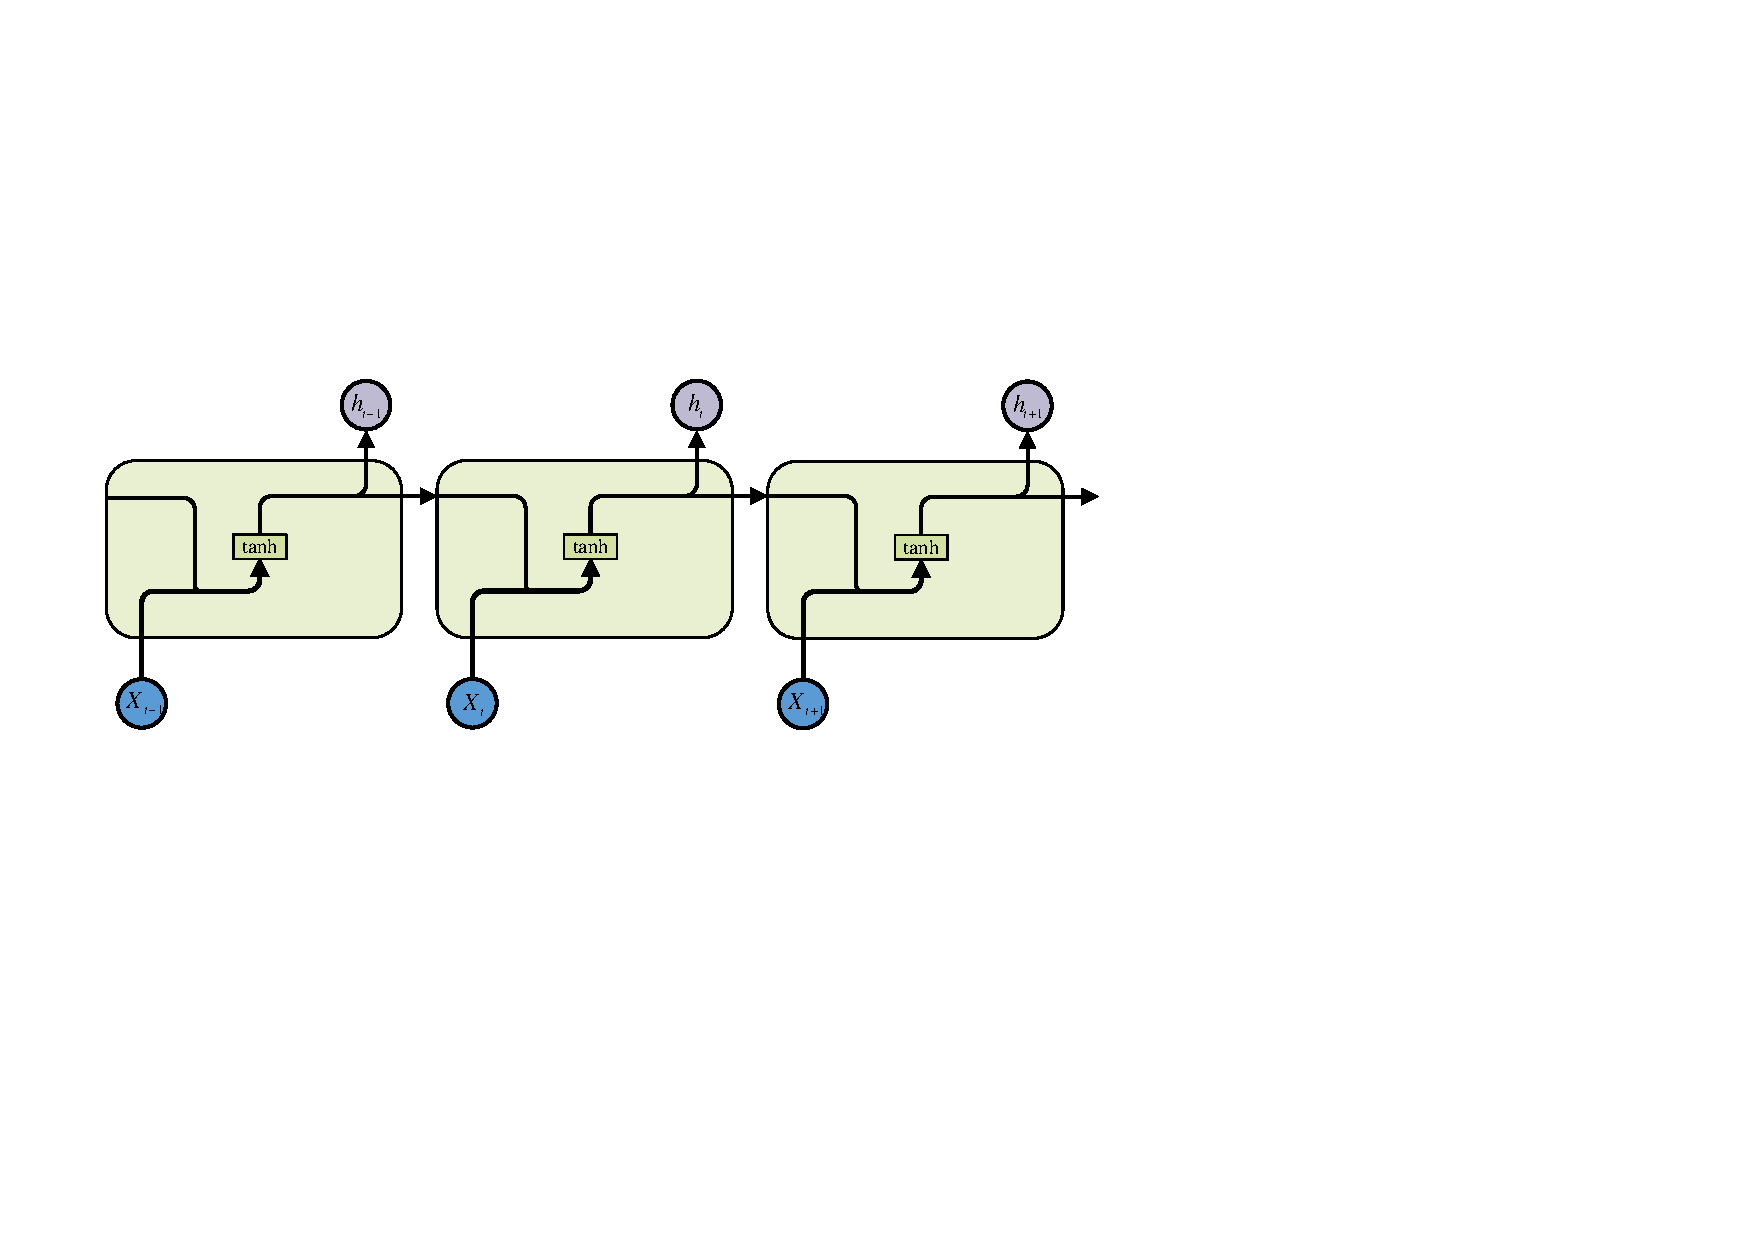
\includegraphics[width=0.8\textwidth]{./pic/SimpleRNN.pdf}
\caption{标准RNN的重复模块}
\label{Figure.2.3}
\end{figure*}

LSTM的重复模块结构较为复杂,如\ref{Figure.2.4}所示通过设计了三个门控结构实现了长期依赖,并大幅缓解了梯度消失和梯度爆炸问题。
\begin{figure*}[!ht]
\centering 
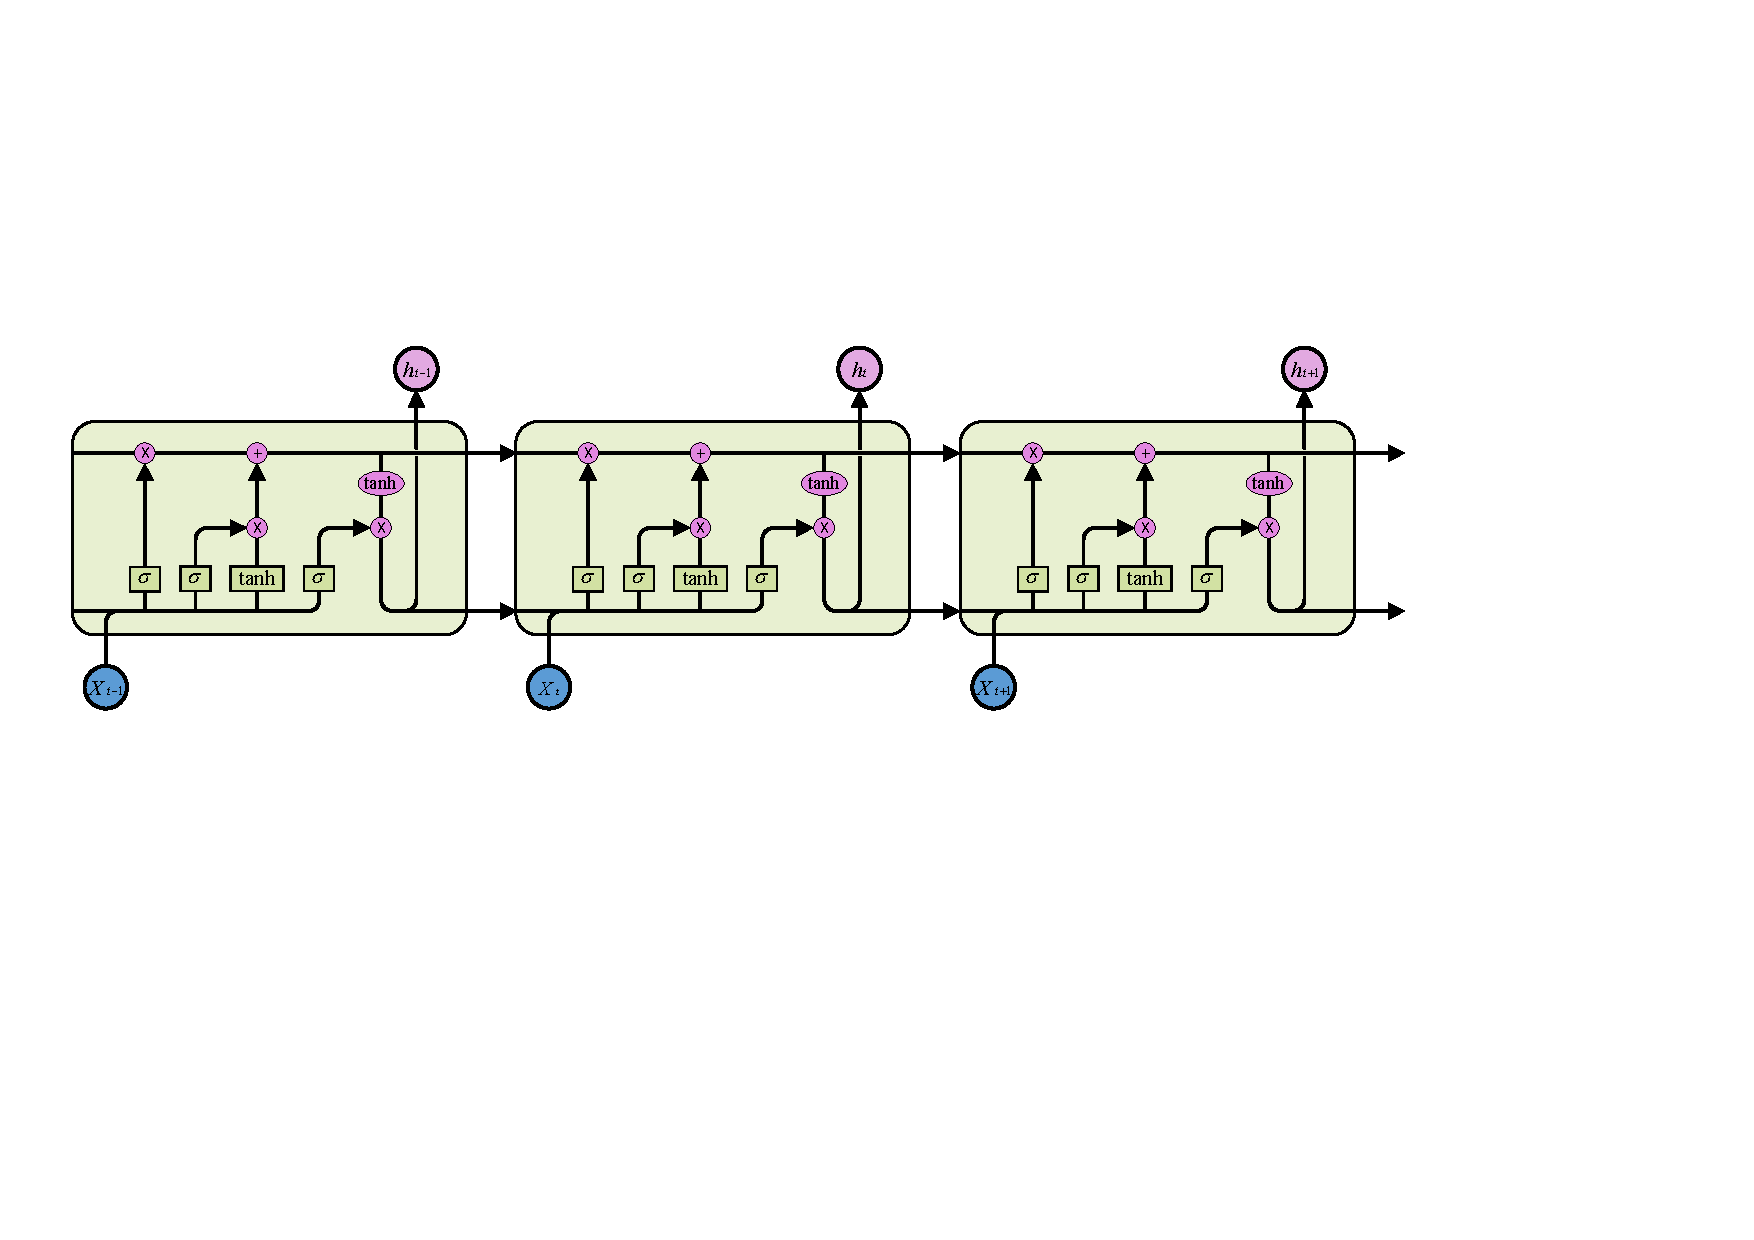
\includegraphics[width=1.0\textwidth]{./pic/LSTM1.pdf}
\caption{LSTM的重复模块}
\label{Figure.2.4}
\end{figure*}

LSTM中最核心的结构是单元状态cell status,单元状态贯穿整个LSTM模型,如图\ref{Figure.2.5}所示,每个重复模块中仅有一些较小的线性相互作用。这样就能够使得信息不变的流动,从而实现长期依赖关系的学习。
\begin{figure*}[!ht]
\centering 
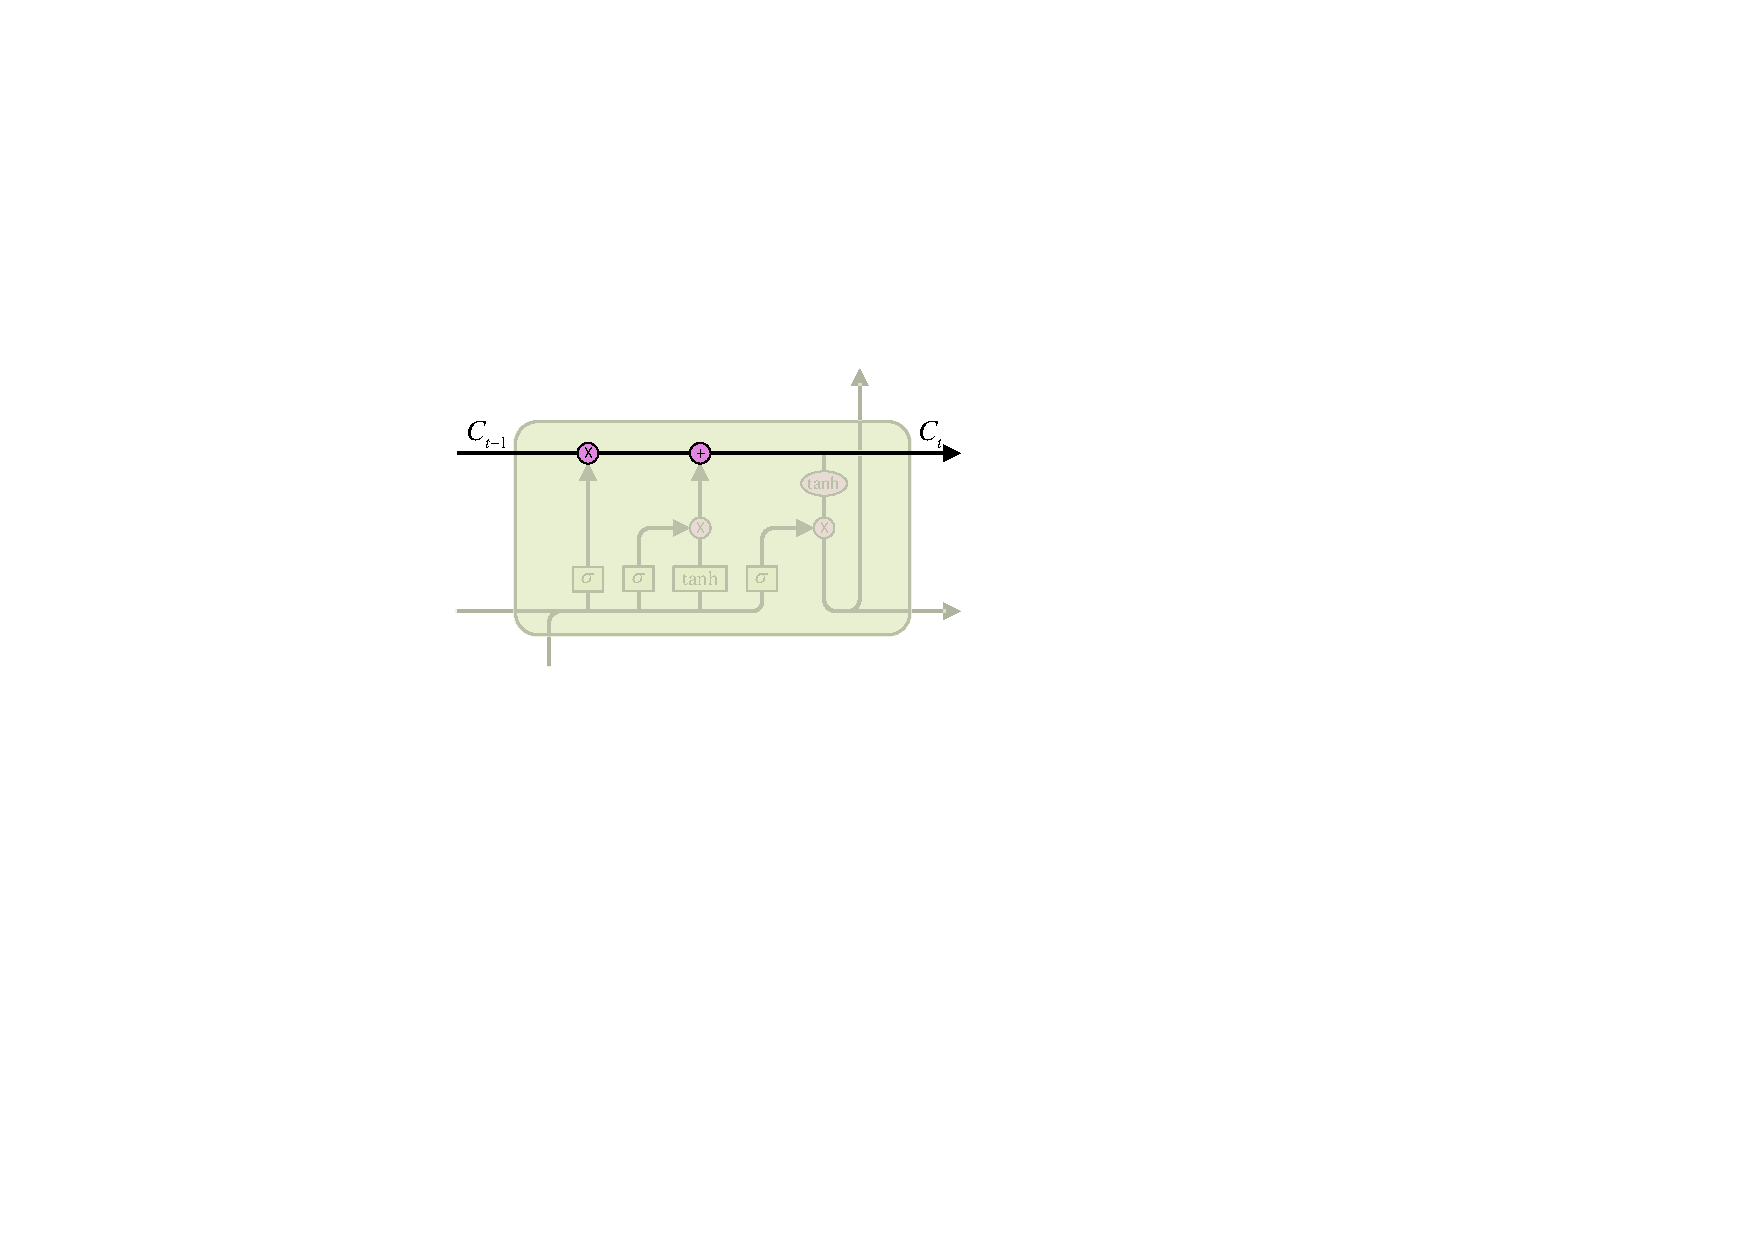
\includegraphics[width=0.5\textwidth]{./pic/LSTM-cell.pdf}
\caption{LSTM的单元状态}
\label{Figure.2.5}
\end{figure*}

LSTM通过每个单元的隐藏状态实现长期记忆,设计了三个门控结构控制单元状态的计算,分别为遗忘门控、记忆门控和输出门控。门控结构是为了实现信息的选择性通过,由以$\mathrm{sigmoid}$函数为激活函数的简单神经网络以及矩阵的逐点运算构成。

遗忘门控的结构如图\ref{Figure.2.6}所示,目的是接受上一个单元状态$C_{t-1}$并通过一个$\mathrm{sigmoid}$层决定保留或者遗忘$C_{t-1}$中的哪些信息。
\begin{figure*}[!ht]
\centering 
\begin{minipage}[b]{0.45\textwidth}
\centering
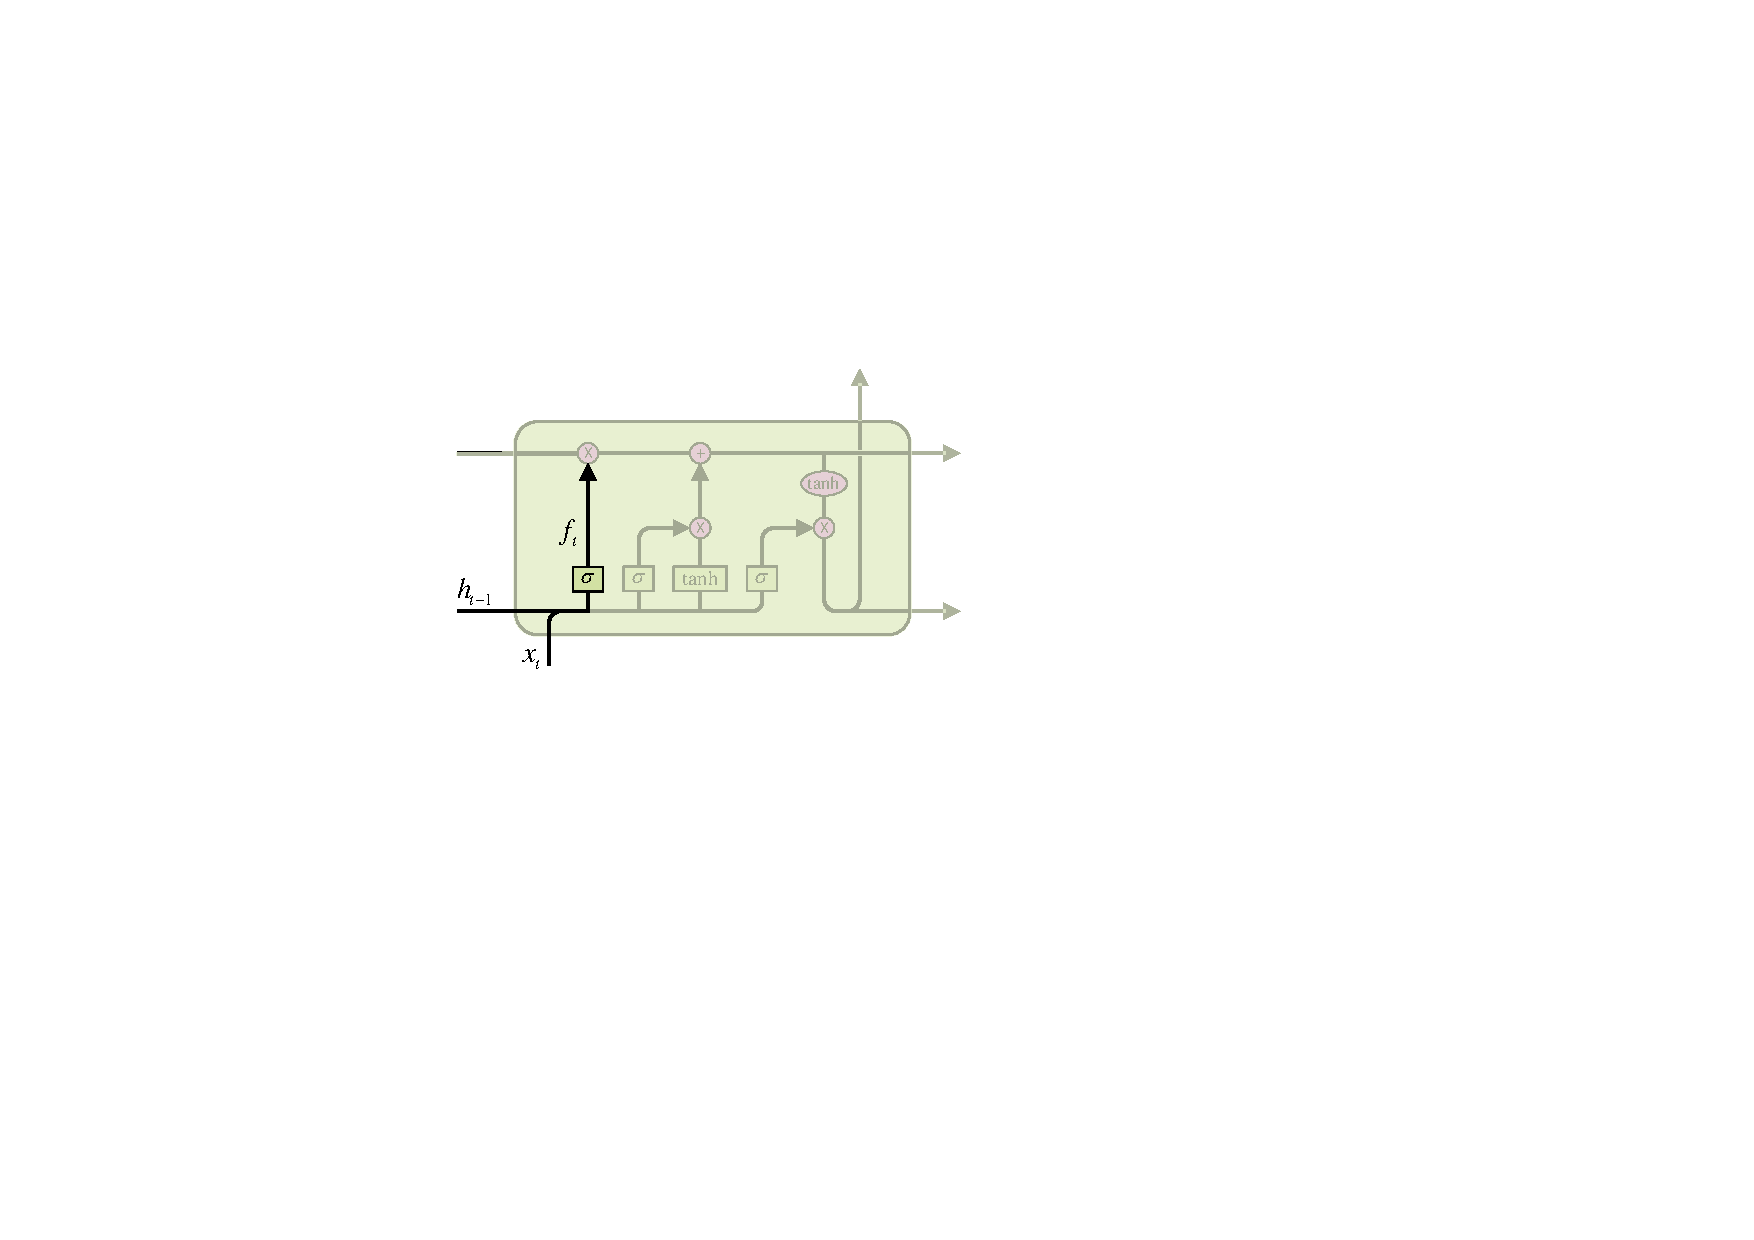
\includegraphics[width=1.0\textwidth]{./pic/LSTM-f.pdf}
\caption{LSTM的遗忘门控}
\label{Figure.2.6}
\end{minipage}
\begin{minipage}[b]{0.45\textwidth} 
\centering 
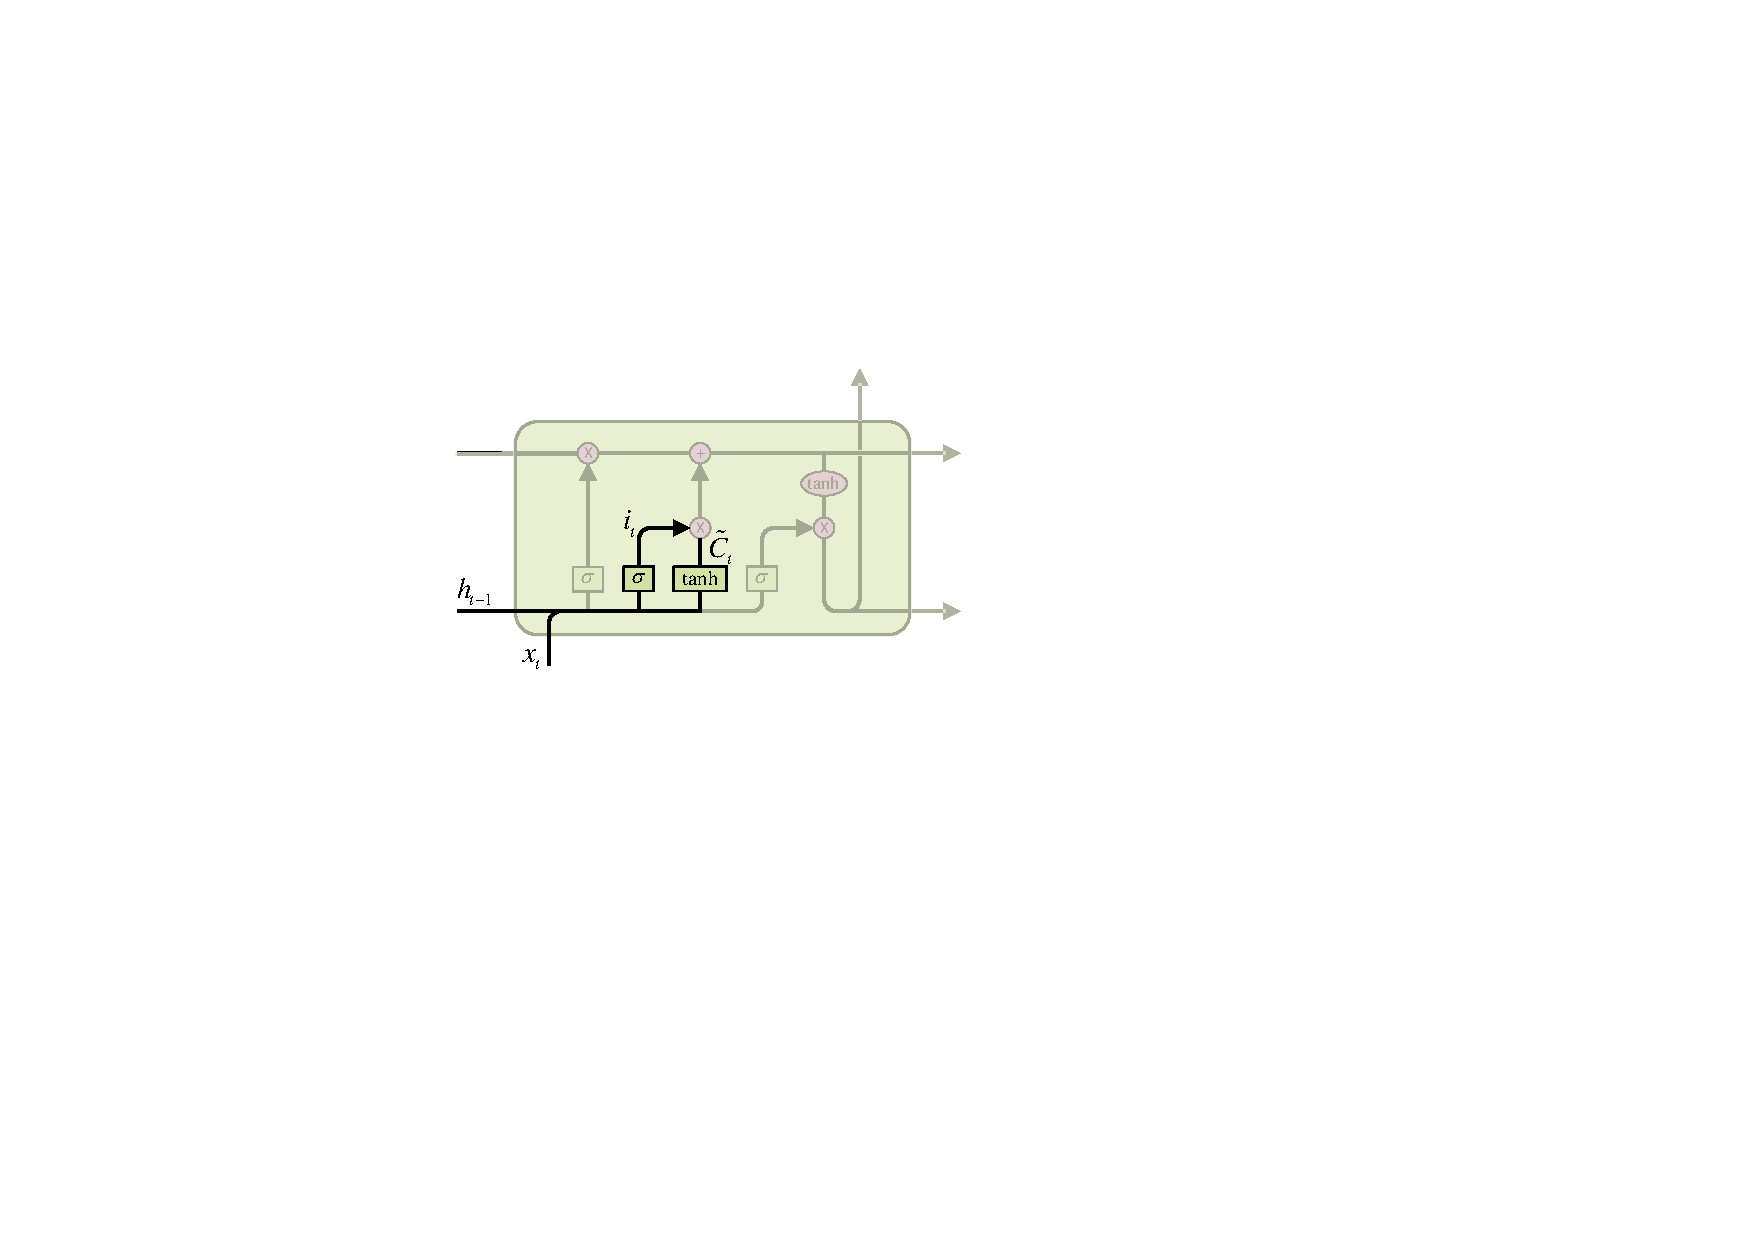
\includegraphics[width=1.0\textwidth]{./pic/LSTM-i.pdf}
\caption{LSTM的记忆门控}
\label{Figure.2.7}
\end{minipage}
\end{figure*}
\begin{equation}
   f_{t} = \sigma(W_f\cdot[h_{t-1},x_{t}]+b_f)
\end{equation}

其中所使用的激活函数为$\mathrm{sigmoid}$函数,将遗忘因子$f_t$值被限制在$[0,1]$之间表示对$C_{t-1}$的保留程度,0表示完全遗忘,1表示完全保留。$f_t$与$C_{t-1}$通过逐元素相乘的哈达玛积进行计算。哈达玛积是矩阵乘法的一种,用符号$\odot$表示,对于两个同阶矩阵$A=(a_{ij})$和$B=(b_{ij})$,其哈达玛积为$C=A\odot B=(c_{ij})$,且$C_{ij}=a_{ij}\times b_{ij}$。

记忆门控则是为了确定该将什么样的新信息存放到单元状态$C_t$中,因此记忆门控包括了一个$\mathrm{sigmoid}$层和一个$\mathrm{tanh}$层,如图\ref{Figure.2.7}所示。$\mathrm{sigmoid}$层的作用与遗忘门控中相同,计算得到记忆因子$i_t$来决定需要更新的信息,$\mathrm{tanh}$层则是根据当前时间步的输入信息$x_t$得到新的候选值向量。
\begin{equation}
   i_{t} = \sigma(W_i\cdot[h_{t-1},x_{t}]+b_i)
\end{equation}
\begin{equation}
   \tilde{C_{t}} = \mathrm{tanh}(W_C\cdot[h_{t-1},x_{t}]+b_C)
\end{equation}

其中短期记忆$\tilde{C_{t}}$使用$\mathrm{tanh}$作为激活函数,与RNN中的$\mathrm{tanh}$层作用相同。

\begin{figure*}[!ht]
\centering 
\begin{minipage}[b]{0.45\textwidth}
\centering
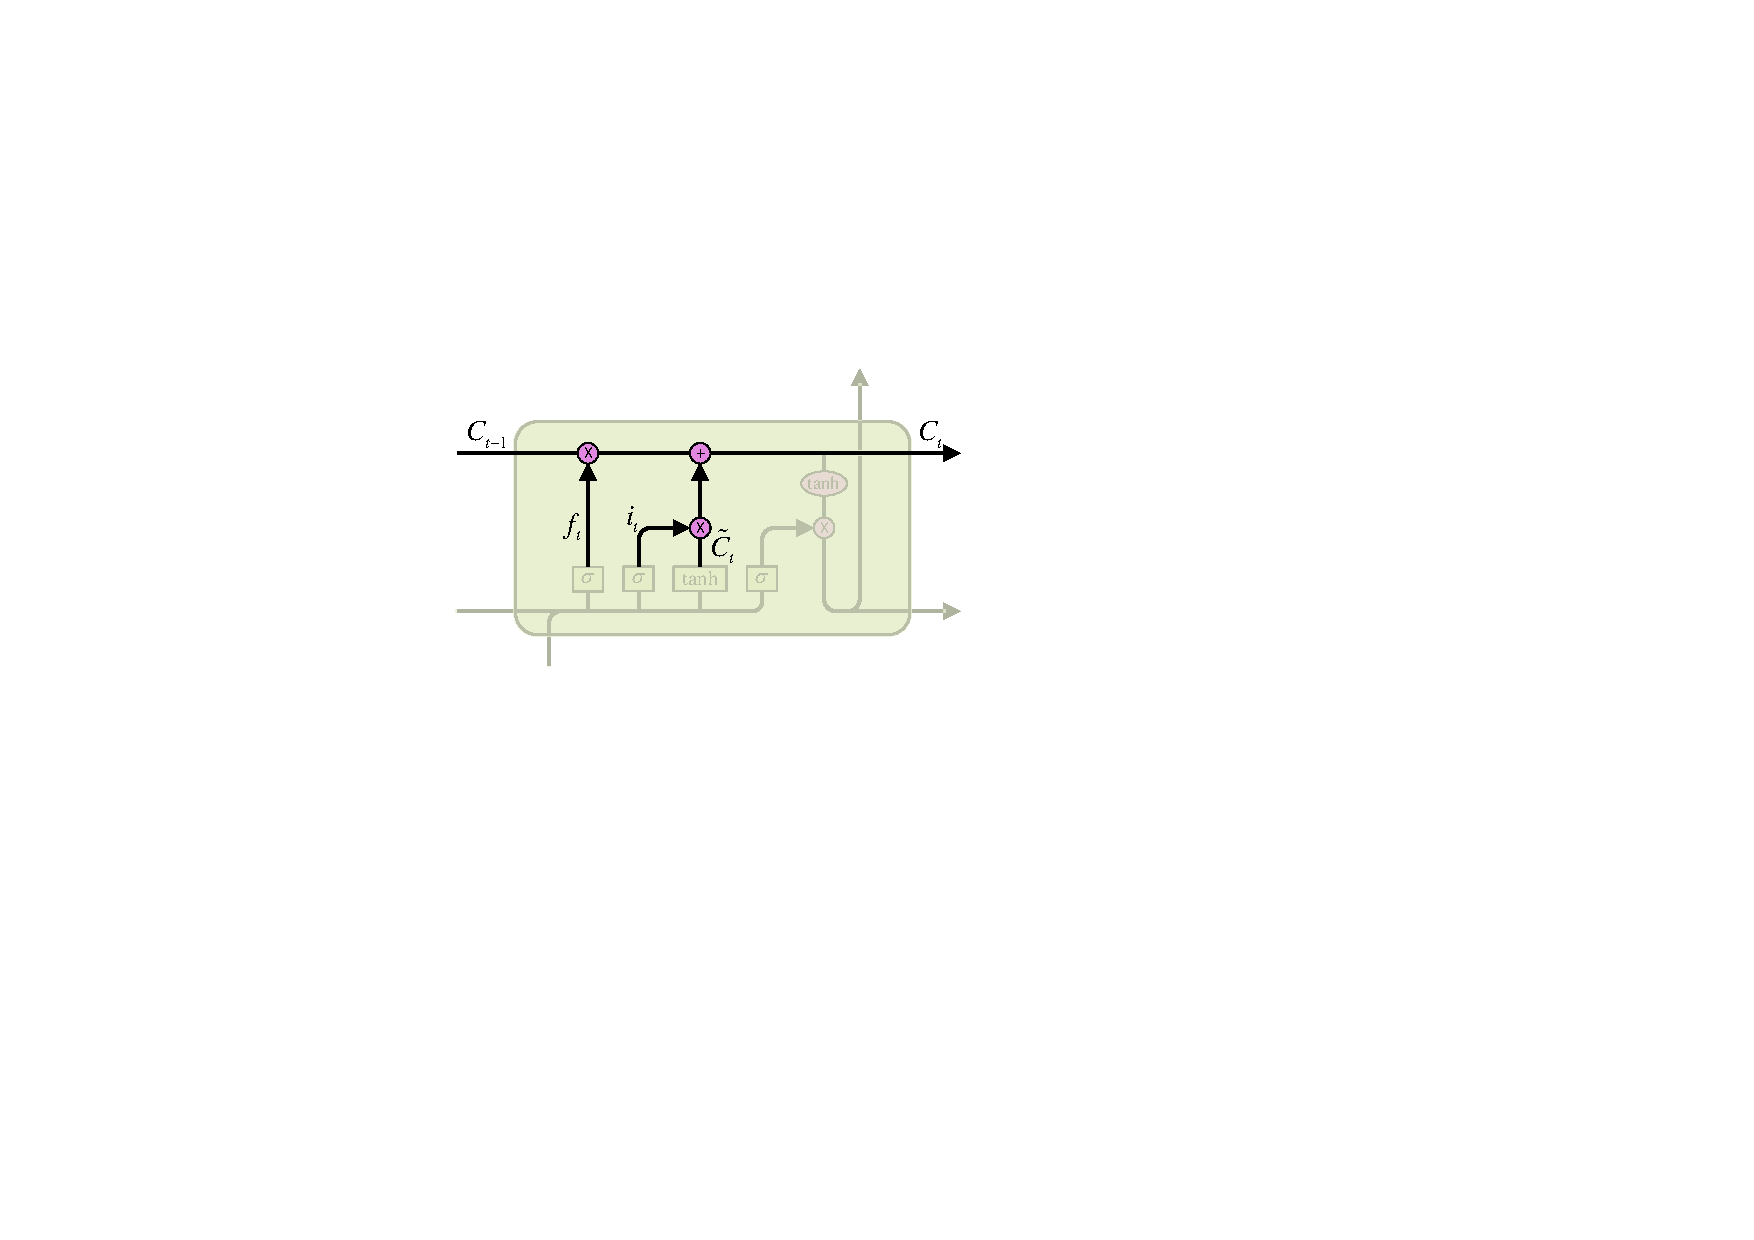
\includegraphics[width=1.0\textwidth]{./pic/LSTM-C.pdf}
\caption{LSTM中更新单元状态}
\label{Figure.2.8}
\end{minipage}
\begin{minipage}[b]{0.45\textwidth} 
\centering 
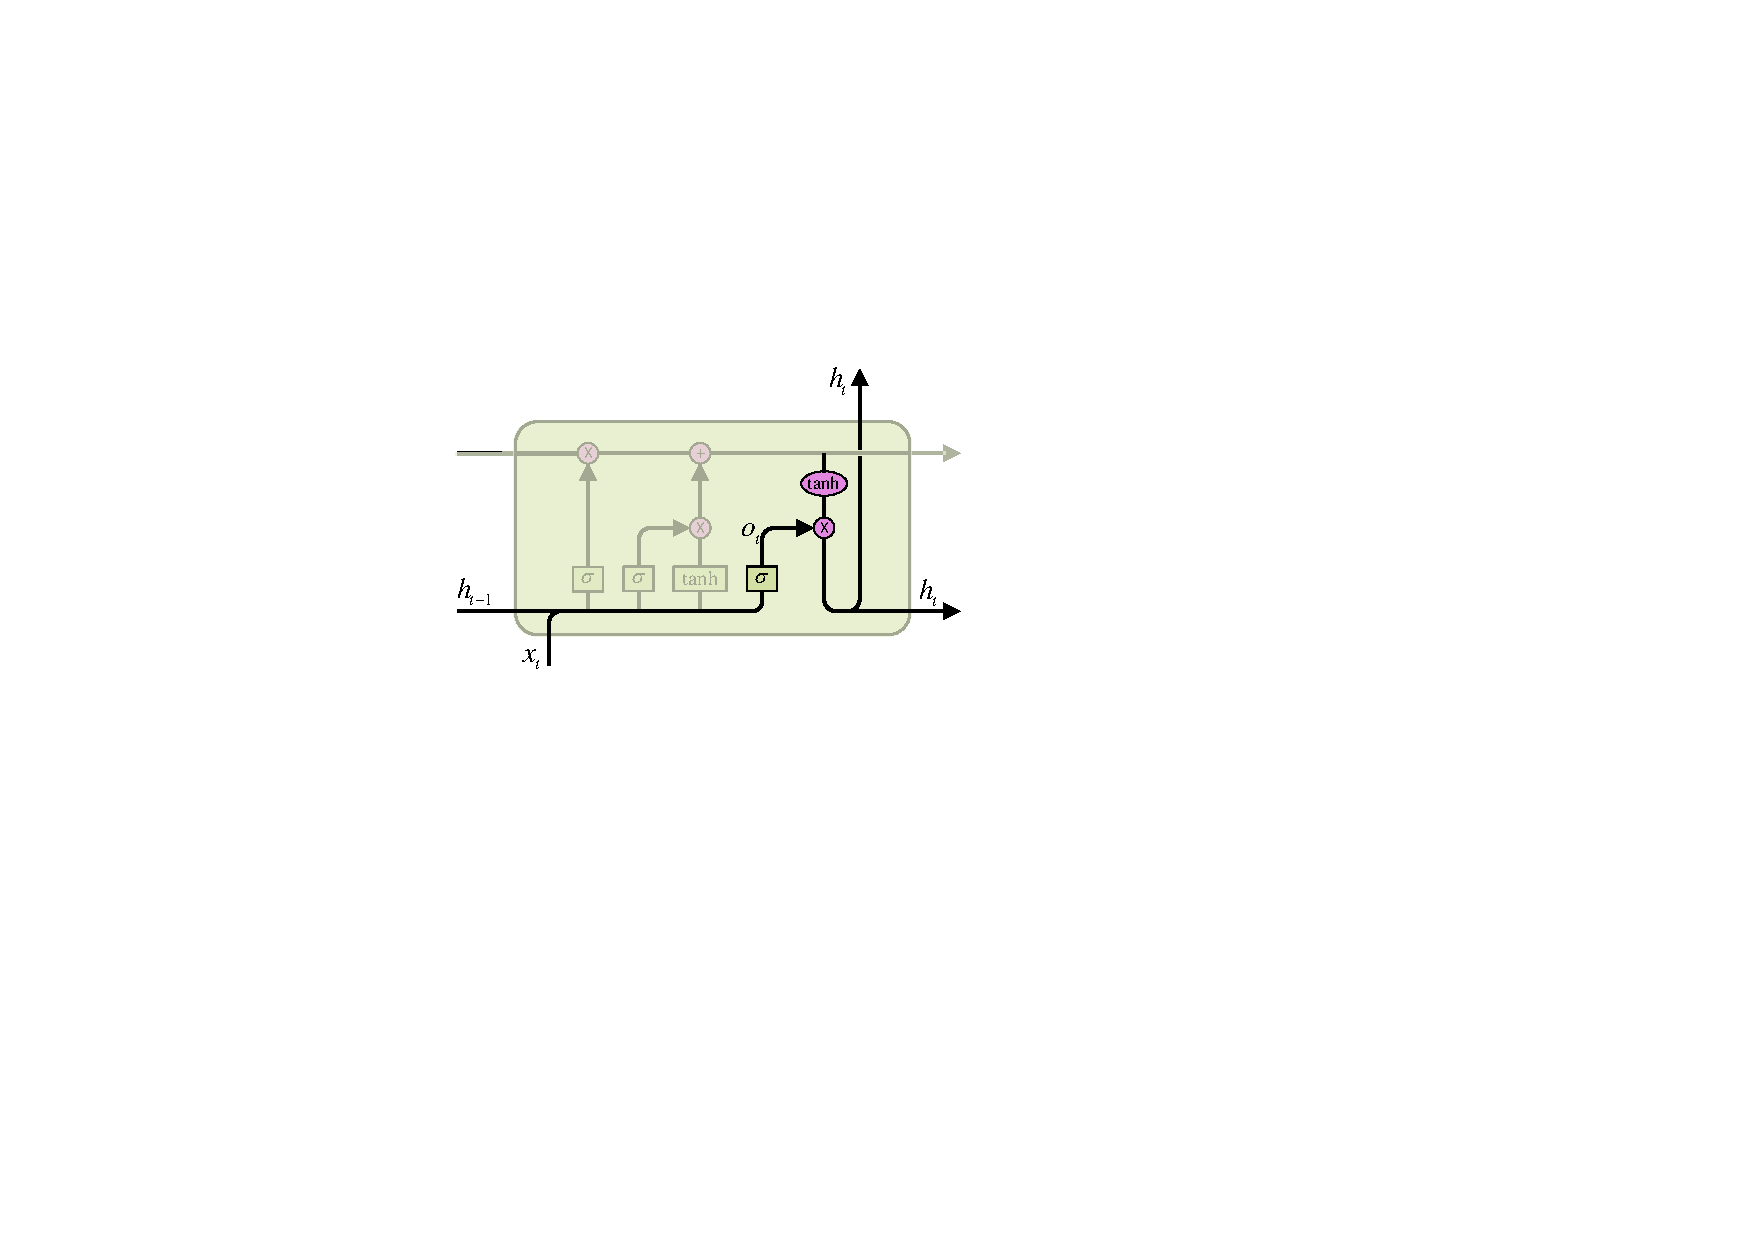
\includegraphics[width=1.0\textwidth]{./pic/LSTM-o.pdf}
\caption{LSTM的输出门}
\label{Figure.2.9}
\end{minipage}
\end{figure*}
在计算得到遗忘因子$f_t$、记忆因子$i_t$和短期记忆$\tilde{C_{t}}$后,两种因子通过哈达玛积分别作用在上一个单元状态$C_{t-1}$和短期记忆$\tilde{C_{t}}$上,得到的结果通过逐元素相加得到当前的单元状态$C_t$,如图\ref{Figure.2.8}所示。
\begin{equation}
   C_{t} = f_t \odot C_{t-1} + i_t \odot \tilde{C_{t}}
\end{equation}

最后根据当前单元状态$C_t$以及当前时间步的输入信息$x_t$计算输出向量。如图\ref{Figure.2.9}所示,一个$\mathrm{sigmoid}$层计算输出因子$o_t$,一个$\mathrm{tanh}$层根据单元状态给出候选值向量,最后相乘得到输出向量$h_t$,计算公式为:
\begin{equation}
   o_{t} = \sigma(W_o\cdot[h_{t-1},x_{t}]+b_o)
\end{equation}
\begin{equation}
   h_t = o_t \odot \mathrm{tanh}(C_t)
\end{equation}

LSTM模型改善了RNN中存在的长期依赖问题,通过结构设计在一定程度上避免了RNN中连乘带来的梯度消失和梯度爆炸问题。在实际应用中的表现通常能够比RNN及HMM模型好,且因为其非线性的特性能够用于复杂深度神经网络的构造,在各领域均有着广泛的应用。但LSTM并没有完全解决长期依赖问题,在$10^3$量级以上的序列上长期依赖问题任然存在。同时因为结构较为复杂,参数量较RNN成倍增加,模型训练计算量很大,训练难度较大。

针对LSTM存在的问题,cho等人\citing{DBLP:conf/emnlp/ChoMGBBSB14}在LSTM进行了改进提出了门控循环单元(GRU),优化了模型参数量以及训练难度。为了更好的阐述本文提出的模型结构,GRU模型在第三章中进行介绍。

\subsection{分类任务及其评价指标}
与POI推荐任务类似,本文将聚集预测任务等价为用户的区域预测,也就是无标签的多分类任务。本小节对分类任务的定义及相关评价指标进行介绍。

\subsubsection{分类任务}
在机器学习和深度学习的各项任务主要分为分类任务和回归任务。其中分类任务主要对离散值进行预测,输出结果为是、否或所属类别;回归任务则对连续值进行预测,得到的输出为确定数值。

分类就是将要预测的数据进行建模,针对给定的输入数据预测其所属类别。从模型角度看,所学习的就是如何将输入数据映射到特定类别。因此对所有类别需要将其映射为数值,如较为常用的one-hot标签、数值标签等,为每个类别分配唯一的对应数值或表示方式。对类别标签的设置目前没有通用的理论支撑,不同的标签映射会影响模型性能,本文第四章通过设计类别标签映射方式取得了一定的性能提升。

分类任务主要分为二分类任务和多分类任务,某些特殊场景下还会用到多标签分类任务、样本不平衡分类任务。

二分类任务是指只有两个类别标签的分类任务,通常视为正类和负类。如常见的垃圾邮件检测,正类为非垃圾邮件,负类为垃圾邮件。二分类通常将类别标签设置为0和1,使用每个样本的伯努利概率分布模型进行建模。输出结果则为样本对应的每个类别的概率,所属类别通过预测概率判断。

多分类任务则具有两个以上类别标签,多分类中类别之间并非对立关系。多分类任务同样是预测每个类别的范畴分布概率对多分类任务进行建模。

多分类任务的类别标签设置通常采用连续数值或one-hot表示。其中one-hot使用一对一映射,在评价指标计算时更加方便,适用于类别数量较少的情况,当类别数量较多时对计算资源和内存资源要求较高;连续数值则适用于类别数量较多的情况,能够较大程度节省资源要求,但数值之间的关系容易对建模结果造成一定影响。

在深度学习中,常常使用Logistic回归\citing{DBLP:books/lib/HastieTF09}作为最后一层进行二分类,多分类则使用softmax回归。

虽然名字中包含回归,但是Logistic回归是一种分类模型。Logistic回归的假设为给定数据集线性可分,对于$n$个随机变量$x=(x_1,x_2,\dots,x_n)$,于是决策边界可以表示为$w_1x_1+w_2x_2+\dots+w_nx_n+b=0$,根据输入$x$计算出$y$,点$(x,y)$落在分界线之上,则判定类别为1,反之为0。

Logistic回归需要找到分类概率$P(Y=1)$与输入向量$x$的直接关系,然后通过根据概率值来判断类别。为了能够拟合离散变量并保持可微,使用sigmoid函数进行拟合:
\begin{equation}
   y=\frac{1}{1+e^{-(w^{\top}x+b)}}
\end{equation}
\begin{equation}
   \ln\frac{y}{1-y}=w^{\top}x+b
\end{equation}

条件分布概率计算为:
\begin{equation}
   \ln \frac{P(Y=1|x)}{1-P(Y=1|x)}=w\cdot x
\end{equation}
\begin{equation}
   P(Y=1|x)=\frac{exp(w\cdot x)}{1+exp(w\cdot x)}
\end{equation}
\begin{equation}
   P(Y=0|x)=\frac{1}{1+exp(w\cdot x)}
\end{equation}

Softmax回归是在Logistic回归的基础上将离散型随机变量$Y$的取值集合推广到$\{1,2,\dots,k\}$,使用softmax函数计算输出,多分类softmax函数的分布概率计算公式为:
\begin{equation}
   P(Y=k|x)=\frac{exp(w_k\cdot x)}{1+\sum_{k=1}^{K-1}exp(w_k\cdot x)},d=1,2,\dots,K-1
\end{equation}
\begin{equation}
   P(Y=K|x)=\frac{1}{1+\sum_{k=1}^{K-1}exp(w_k\cdot x)}
\end{equation}

\subsubsection{常用评价指标}
分类任务常用的评价指标为准确率、精确率、召回率、F1分数、ROC、AUC等,针对不同任务常使用不同的评价指标,本文的主要评价指标为多分类\citing{DBLP:conf/acml/YangLCL19}召回率$recall@k$和AUC。

为了能够更好的介绍评价指标的定义,先对于二分类任务中常用的$recall$指标进行介绍。

在二分类任务中所有样本存在四种情况:真正例(TP)为模型预测为正的正样本;假正例(FP)为模型预测为正的负样本;假负例(FN)为模型预测为负的正样本;真负例(TN)为模型预测为负的负样本。

最为直观的评价指标为准确率,表示预测正确的样本占总样本的百分比:
\begin{equation}
   Accuracy=\frac{TP+TN}{TP+TN+FP+FN}
\end{equation}

但在样本数据的类别不均衡的情况下,占比较大的类别对准确率的影响更大,此时准确率结果并不能起到评价分类器好坏的作用。

在准确率的基础上,精确率计算的是自所有被预测为正的样本中实际为正样本的概率,比较适合进行挑选的任务。
\begin{equation}
   Precision=\frac{TP}{TP+FP}
\end{equation}

召回率$recall$则针对所有样本,计算样本的所有正例中有多少被正确预测。
\begin{equation}
   Recall=\frac{TP}{TP+FN}
\end{equation}

由于本文的任务中区域之间并没有直接关联,模型的出发点为尽可能准确预测在目标区域的用户,因此使用召回率更为合适。虽然F-1分数同时兼顾了精确率和召回率,但在本文场景中的适用性不如召回率。

而在多分类任务中召回率$recall$的计算相对较为复杂,首先需要根据所有预测结果计算每个类别的对应的$recall$值为$(recall_0,recall_1,\dots,recall_n)$。同时为了能够评估模型的整体性能,需要对所有类别进行综合考虑。Macro-recall指标直接对所有$recall$值求平均,但会在一定程度上受到数据集分布的影响。Micro-recall指标则是对数据集中的所有样本计算全局混淆矩阵,虽然Micro-recall会在一定程度上受到不均衡类别的影响,但更符合聚集预测任务中聚集区域样本数量更多的诉求。
\begin{equation}
   Recall_{micro}=\frac{\bar{TP}}{\bar{TP}+\bar{FN}} = \frac{\sum_{i=1}^n TP_i}{\sum_{i=1}^n TP_i+\sum_{i=1}^n FN_i}
\end{equation}

由于分类数量较多,为了能够更好的衡量模型性能,本文考虑使用$recall@k$,即当被预测样本的标签被预测的前$k$个结果命中时认为其被正确预测了。能够根据不同的$k$值对模型性能进行多维度的衡量。

同时为了能够更好的描述模型整体性能,本文使用AUC指标(Area under the Curve of ROC)\citing{DBLP:journals/prl/Fawcett06}作为辅助,AUC表示每一类别中正例排在负例前面的概率,在大多数情况下能够较好的衡量模型的整体建模性能。由于其基于ROC曲线进行计算,就不再次展开介绍。

\section{时空特征建模方法}
本节对后续章节中所涉及的位置预测中的时空特征提取和基于图网络的交通流量预测模型进行介绍,对算法特点和局限性进行分析,为本文所提出的模型方法的介绍做铺垫。

\subsection{基于时空特征的循环神经网络}
在轨迹预测任务中对所有用户建立准确的预测模型是较难的,这是因为轨迹预测任务中使用的数据集较为稀疏,用户轨迹之间相互影响较小。但对每个用户建立一个预测模型是比较可行的方案。因此,大部分轨迹预测任务基于单个用户建模,基于时空特征的循环神经网络(STF-RNN)就是在此基础上通过对RNN模型进行扩展,结合查找表层自动提取时间和空间特征。

\begin{figure*}[!ht]
\centering 
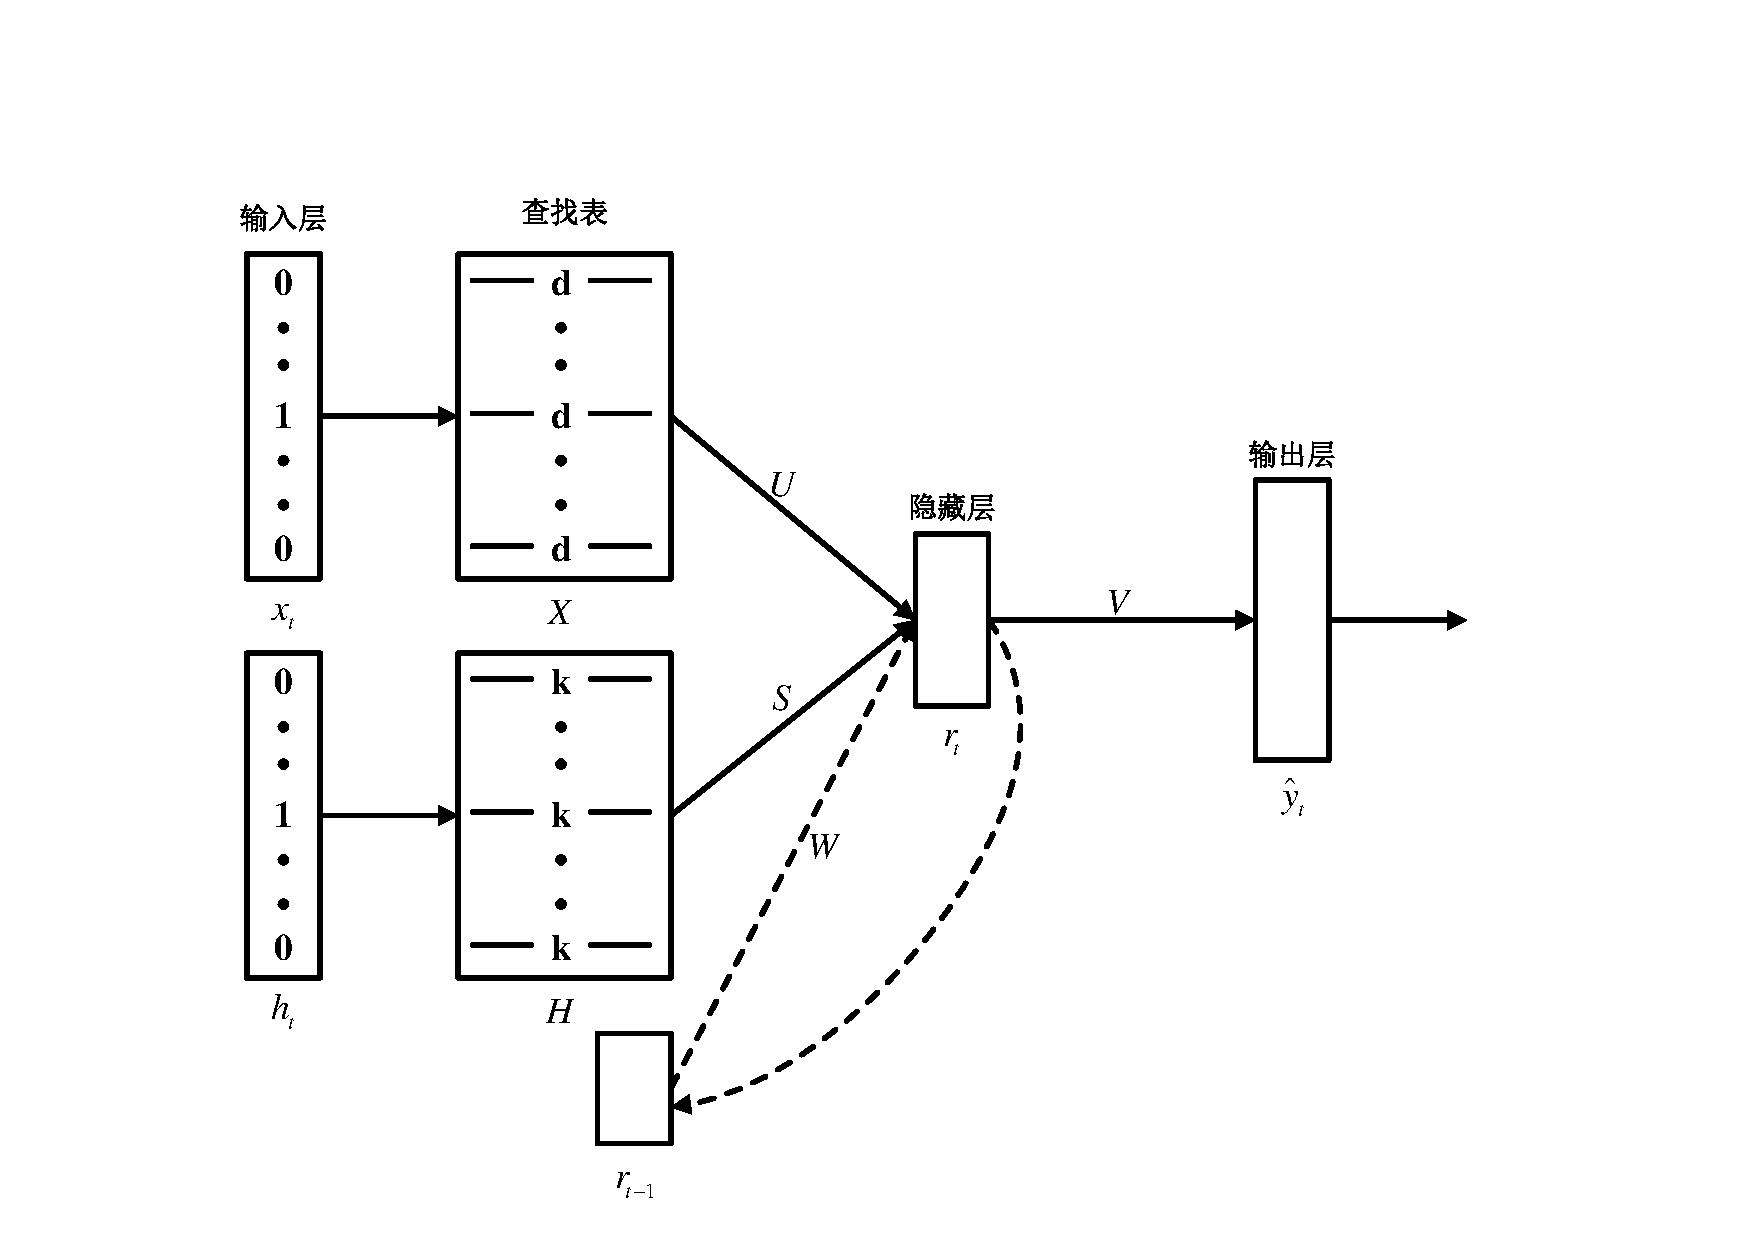
\includegraphics[width=0.7\textwidth]{./pic/stf-rnn.pdf}
\caption{STF-RNN模型结构}
\label{Figure.2.10}
\end{figure*}
STF-RNN主要考虑两类特征,一是用户每个位置对应的ID信息,使用1-of-N进行编码;二是$t$时间时离开兴趣点的小时数,同样使用1-of-N进行编码。整体结构如图\ref{Figure.2.10}所示,由两个查找表层和一个RNN层构成。

首先通过查找表层将中心ID的向量和离开时间映射为实值向量。目的是学习兴趣点和离开时间的输入特征中的有效表示。这种表示方式使模型能够捕捉到用户行为的语义信息。

在RNN层中当前的输入以及隐藏层的上一个状态用于计算隐藏层的下一个状态。因此,下一个位置预测不仅取决于当前所处的位置,还受到历史轨迹序列的影响。RNN结构有助于根据用户的移动历史并发现移动之间存在的依存关系,从而提高模型的性能。

目前看来这样的处理方式无疑是较为粗糙的,但SF-RNN模型是最先使用RNN建模时空特征的工作之一。摆脱了诸多马尔可夫链通过手工构建转移矩阵提取时空特征的方式,实现了自动的时空特征提取。充分发挥了神经网络模型的优势,通过训练能够自动发现一些用户行为模式中的依存关系。

\subsection{分层时空长短时记忆网络}
大多数顺序模型仅强调节点之间的依赖性,而忽略了空间和时间关系之列的其他对应关系,因此大多数深度学习模型中均存在数据稀疏性问题。分层时空长短时记忆网络(HST-LSTM)尝试在LSTM上进行扩展,实现了对时空特征的提取,并验证了时空依赖性对缓解数据稀疏性问题至关重要。

HST-LSTM的核心改进为在LSTM的基础上引入了空间影响因子和时间影响因子,对LSTM中三个门控进行了如下设计:
\begin{equation}
   i_t= \sigma(W_{i}l_t + W_{h_i}h_{t-1} + F_i(s_{t-1}, q_{t-1}) + b_i)
\end{equation}
\begin{equation}
   f_t= \sigma(W_{f}l_t + W_{h_f}h_{t-1} + F_f(s_{t-1}, q_{t-1}) + b_f)
\end{equation}
\begin{equation}
   o_t= \sigma(W_{o}l_t + W_{h_o}h_{t-1} + F_o(s_{t-1}, q_{t-1}) + b_o)
\end{equation}

时空影响因子的计算函数$F(\cdot)$基于加法算子实现:
\begin{equation}
   F_k(s_{t-1},q_{t-1})=W_{sk}s_{t-1} + W_{qk}q_{t-1},k=i,f,o
\end{equation}

其中$W_{sk},W_{qk} \in \mathbb{R}^{|c|*d}$是关于时空因素的线性转换矩阵,$|c|$是单元数。

此外在使用时间间隔$v_q$或者地理距离$v_s$计算相应的向量时通过将数值划分为离散间隙并仅对其上下限进行编码来降低对间隔建模时的稀疏性问题。

虽然HST-LSTM针对时空特征进行了单独的处理,仍然只是简单地融合到各个门控中,并未对其进行显式建模。这样的方式并不能充分发挥时空特征对建模行为模式的作用,HST-LSTM通过会话场景等方案设计进行改进,但适用性较差。

\subsection{时空门控网络}
时间门控网络(STGN)是为了解决更充分提取并使用时空特征而提出的。RNN扩展模型中均不适用于长期兴趣依赖,又如HST-LSTM这类并未对LSTM结构针对时空特征建模进行设计的模型同样难以建模长期时空特征。STGN通过增强LSTM设计了两对时间门控和距离门口,分别控制短期兴趣和长期兴趣依赖。

\begin{figure*}[!ht]
\centering 
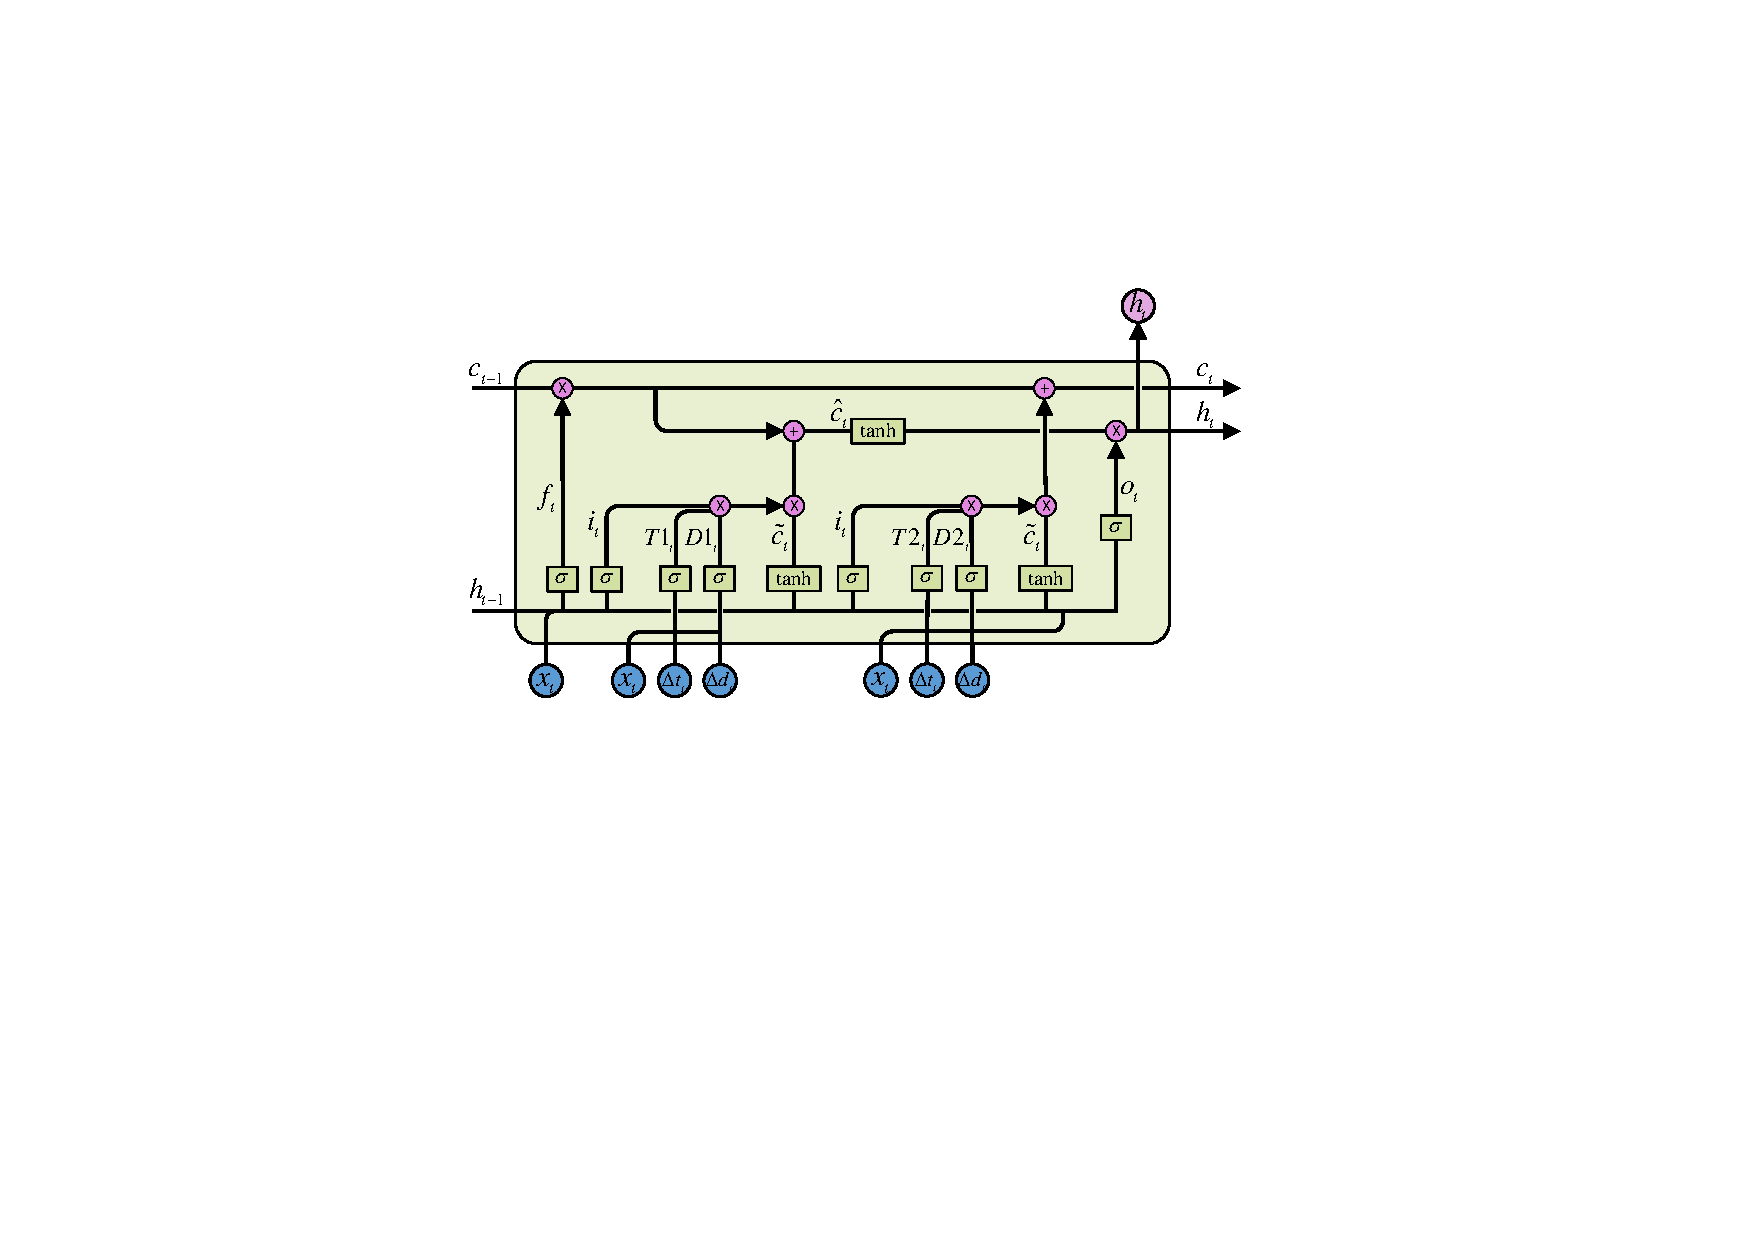
\includegraphics[width=0.6\textwidth]{./pic/stgn.pdf}
\caption{STGN单元结构}
\label{Figure.2.11}
\end{figure*}
如图\ref{Figure.2.11}所示,STGN设计了两对两个时间门控和两个距离门控,分别表示为$T1_t,T2_t,D1_t,D2_t$。$T1_t,D1_t$用于控制最近访问的地点对下一步行动的影响。STGN在LSTM基础上的公式修改为:
\begin{equation}
   T1_t=\sigma(x_tW_{xt_1}+\sigma(\Delta t_tW_{t_1})+b_{t_1})
\end{equation}
\begin{equation}
   T2_t=\sigma(x_tW_{xt_2}+\sigma(\Delta t_tW_{t_2})+b_{t_2})
\end{equation}
\begin{equation}
   D1_t=\sigma(x_tW_{xd_1}+\sigma(\Delta d_tW_{d_1})+b_{d_1})
\end{equation}
\begin{equation}
   D2_t=\sigma(x_tW_{xd_2}+\sigma(\Delta d_tW_{d_2})+b_{d_2})
\end{equation}

$T2_t,D2_t$两个门控的目的是利用时间间隔和距离间隔模拟用户的长期兴趣。并添加了一个新的单元状态$\hat{c_t}$记忆短期兴趣。$c_t$不仅可以记住用户的历史访问的顺序,还可以记住相邻POI之间的时间和距离间隔信息,从而捕捉用户的长期兴趣。$\hat{c_t}$和$c_t$的计算公式为:
\begin{equation}
   \hat{c_t}=f_t\odot c_{t-1}+i_t \odot T1_t \odot D1_t \odot \tilde{c_t}
\end{equation}
\begin{equation}
   c_t=f_t \odot c_{t_1}+i_t \odot T2_t \odot D2_t \odot \tilde{c_t}
\end{equation}

$o_t$和$h_t$也进行了相应的修改:
\begin{equation}
   o_t=\sigma(W_o[h_{t-1},x_t]+\Delta t_tW_{to}+\Delta d_tW_{do}+b_o)
\end{equation}
\begin{equation}
   h_t=o_t \odot \tanh(\hat{c_t})
\end{equation}

对距离间隔进行建模可以帮助捕获用户的总体空间兴趣,而对时间间隔进行建模则可以帮助捕获用户的周期性访问行为,通过对时间间隔和距离间隔的显式建模,放大了时空特征对整体行为模式的影响。

STGN模型虽然考虑了时空特征但仍仅适用于弱实时轨迹和对单个用户进行建模,难以捕获用户之间的时空关系,且因为其扩展了两对门控和一个单元状态,参数量较LSTM成倍的增加。本文基于STGN的局限性进行优化,提出了更适用于强实时轨迹建模的STGRU模型。

\subsection{时空图卷积网络}
上述时空特征建模的方法均基于单个序列进行建模,但在聚集预测任务中需要考虑用户之间的时空依赖性。交通流量预测任务需要同时兼顾群体之间关系及时空特征,时空卷积网络(STGCN)通过构建基于交通流量路网图实现交通流量的预测,结合任务特点将图拓扑结构视为空间特征,并巧妙设计了时间维度特征的提取。

交通流量预测是较为典型的时间序列预测问题,即给定先前的流量观察值作为预测,在接下来的时间步骤中预测最可能的流量测量值。因此,流量的变化受其周边流量的影响很大,具有天然的时空关联性。

为了充分利用空间信息,STGCN通过图来建模交通网络,而不是对单独结点进行处理。为了处理RNN的固有缺陷,在时间轴上采用卷积结构建模时间特征。

\begin{figure*}[!ht]
\centering 
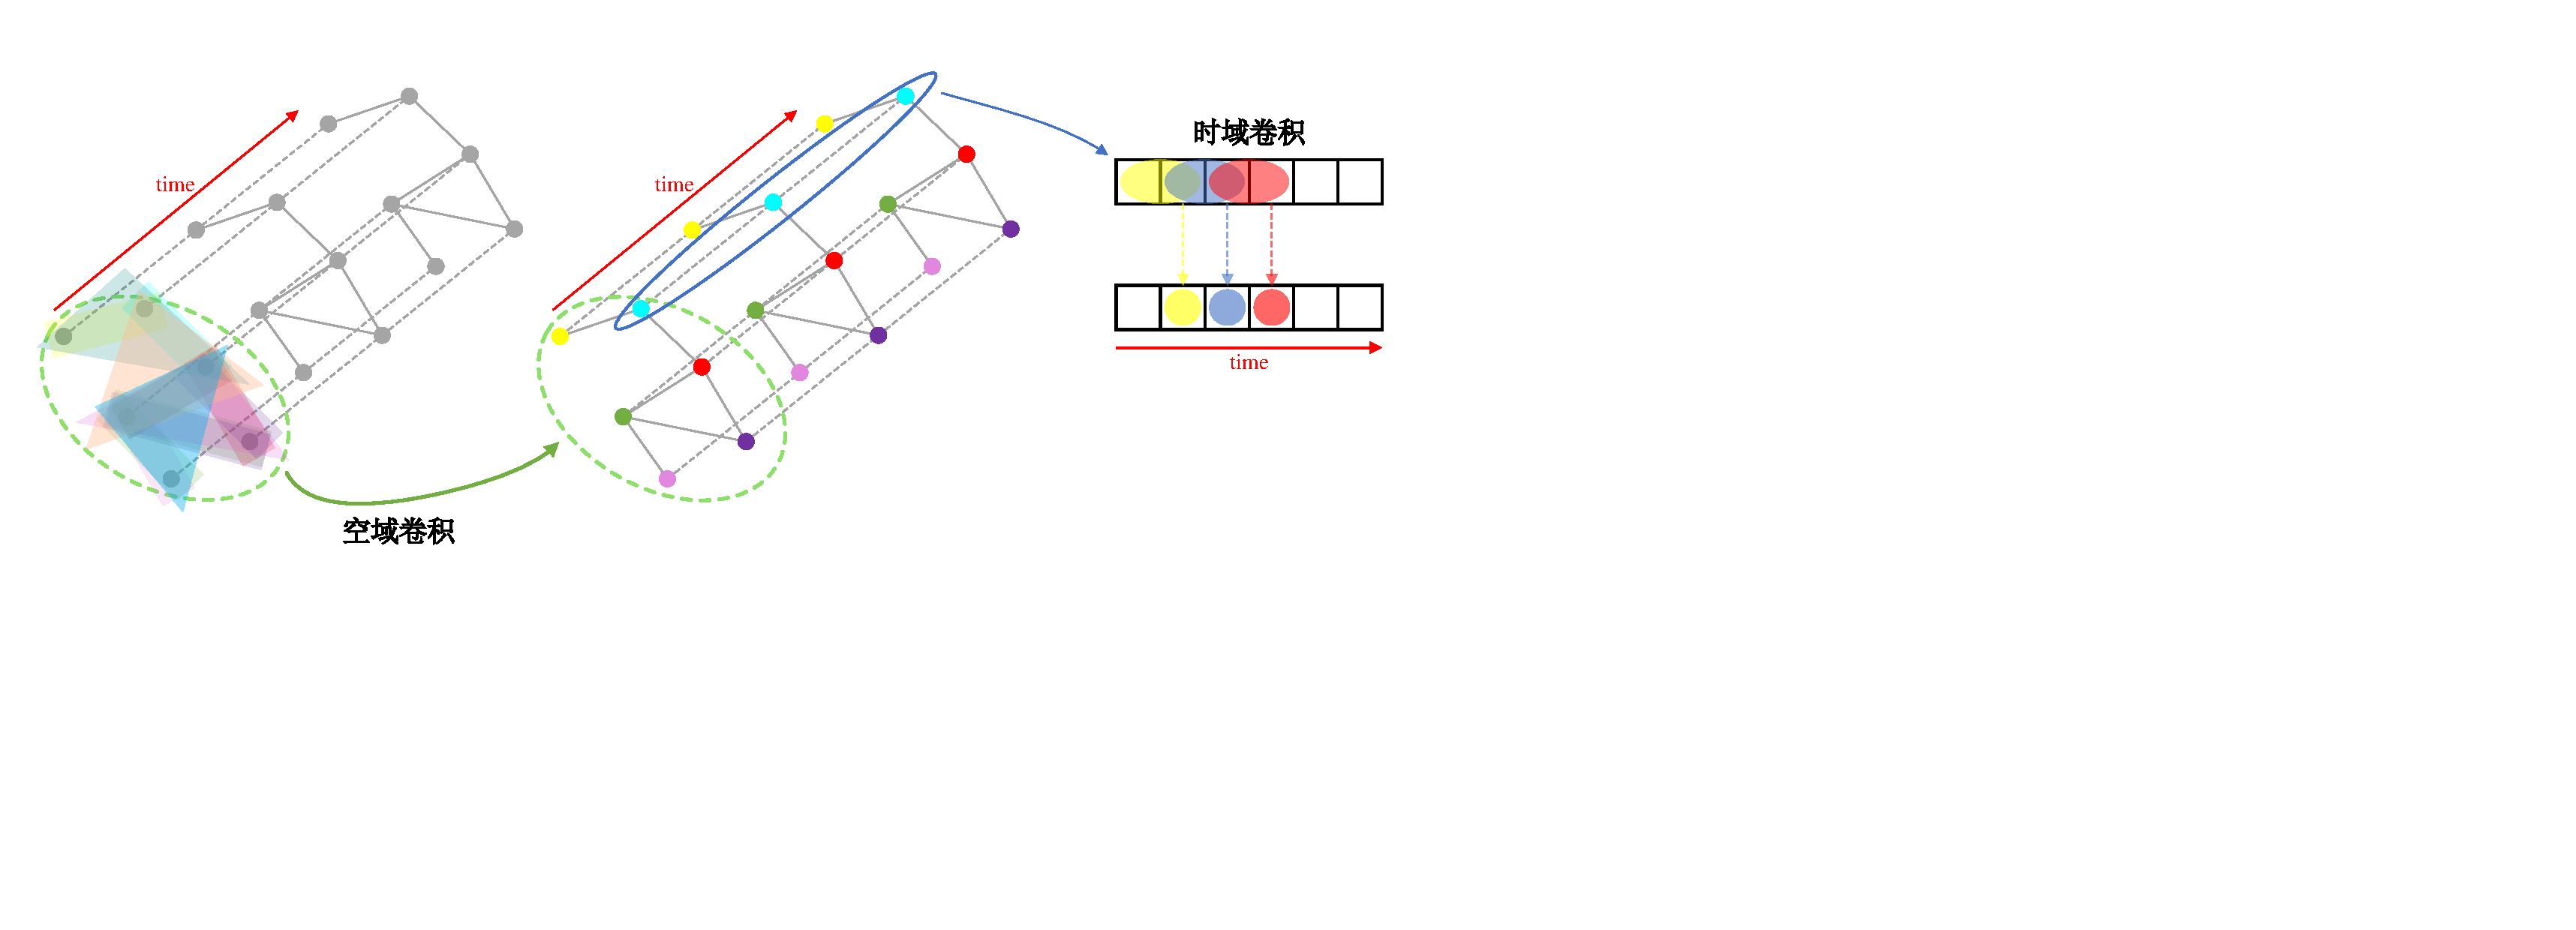
\includegraphics[width=0.8\textwidth]{./pic/astgcn.pdf}
\caption{STGCN原理示意图}
\label{Figure.2.12}
\end{figure*}
如图\ref{Figure.2.12}所示,STGCN由空间维度上的图卷积和沿时间维度的一维卷积组成。根据交通网络构建图结构,每个节点的特征可以看作图上的信号。

为了充分利用交通网络的拓扑特性,在每个时间片上都采用图卷积网络GCN直接处理信号,提取图中的拓扑属性,等价于空间特征提取。时间维度上则是通过标准卷积层提取节点相邻时间片的信息,再与图卷积的结果进行合并更新。

STGCN能够很好的捕捉交通数据的时空特征,且能够同时考虑用户之间的关系,本文第四章中所提出的聚集预测模型便是基于这一思路对用户之间行为模式的建模方式进行设计。

\section{数据集介绍}
由于聚集预测任务的特殊性,对数据集有较高的要求,常规的出租车数据集、少数目标的轨迹数据集等并不适用,因此本文使用了东京大学空间信息科学中心(CSIS)发布的三个基于SNS的人流数据集,人流数据集目标更多和实时性更强,更符合聚集预测任务的应用场景。

\textbf{名古屋人流数据集}(Nagoya People Flow,NPF)包含2013年名古屋地区共2387个用户的轨迹,共有1,068,064个轨迹点。轨迹覆盖时间为6天,分别为7月22日、7月28日、9月16日、9月22日、12月24日和12月29日。每条轨迹覆盖时间为24小时,轨迹点采样时间间隔为5分钟。

\textbf{大阪人流数据集}(Osaka People Flow,OPF)包含2013年大阪地区的4924个用户的轨迹,轨迹覆盖时间为7月22日、7月28日、9月16日、9月22日、12月24日和12月29日,轨迹点总数为2,552,883。

\textbf{东京人流数据集}(Tokyo People Flow,TPF)是三个数据集中最大的一个,包含了2013年东京地区11536个用户的轨迹数据,数量为6,883,245个轨迹点。时间为7月1日、7月7日、10月7日、10月13日、12月16日和12月22日。

上述三个数据集的覆盖时间均包含夏、秋、冬三个季节,每个季节中的两天分别为周末和工作日,包含了不同时间的多种行为模式,能够为后续章节提供较好的实验支撑。

\section{本章小结}
本章对本文中所使用的序列神经网络和时空特征建模算法进行了介绍。首先介绍了序列神经网络相关算法与概念,主要为循环神经网络、长短时记忆网络、分类任务及其评价指标三部分。其次对时空特征建模方法的发展进行阐述,分别介绍了基于时空特征的循环神经网络、分层时空长短时记忆网络、时空门控网络、时空图卷积网络等方法的特点及发展。最后对本文中所使用数据集的特点与详细情况进行介绍,并分析了数据集的选择原因。

\chapter{基于信息融合的轨迹预测算法}
本章首先分析了当前轨迹预测方法存在的问题,并阐述解决问题的思路。其次详细介绍了本章所提出的时空门控循环单元(STGRU)的结构与原理。最后在真实世界的人流轨迹数据集上进行评估,通过实验验证所提出模型的有效性。

\section{引言}
聚集预测主要利用各种物联网传感设备(如手机、汽车和其他GPS设备)所收集的轨迹数据。这些轨迹数据包括多种类型的模式,如步行轨迹、驾驶轨迹和公共交通轨迹等,因此聚集预测需要适用于多类轨迹场景。同时,有别于其他轨迹预测任务,如POI(Point of Interest)推荐,聚集预测任务更关注实时轨迹数据,并具有较强的空间依赖性。但是现有方法主要基于轨迹数据进行建模,在多类轨迹上适用性较差,忽略了地理环境对行为模式的巨大影响。

为了实现更高精度的轨迹预测,目前的方法主要集中在对轨迹数据的顺序以及相邻轨迹点之间的时间间隔和距离间隔进行建模\citing{DBLP:conf/wsdm/LiWM20}。其主要目的是结合时间和空间特征对用户行为模式建模。典型的技术如循环神经网络(RNN)、长短时记忆(LSTM)和门循环单元(GRU)已成功应用于各种类型的序列数据建模,并大大改善了性能。然而,上述方法都没有考虑轨迹数据中的地理信息。最近的一些工作致力于扩展RNN和LSTM,以实现对邻点之间的时间和距离间隔的建模。例如,ST-RNN试图通过扩展RNN来建模时空特征,HST-LSTM将时空影响融入LSTM中。最近,STGN通过设计两对时间门控和距离门控,分别对时间间隔和距离间隔进行建模,实现了SOTA。但性能提升的同时也带来了模型参数量成倍增加的问题。

然而,由于不均匀的采样间隔和传感设备的分布,应用于聚集预测的轨迹数据通常存在数据稀少的问题。以前的工作试图通过时空关系来缓解数据的稀疏性问题,但效果并不明显。受Li等人\citing{DBLP:conf/iclr/LiYS018}的启发,地理环境信息(如路网结构)和外部知识(如天气信息和节假日信息)可以有效缓解数据稀少的问题。其中地理环境的影响对于用户短期和长期行为模式的建模至关重要,天气和假日信息则影响用户的整体行为。例如,如果用户的连续轨迹在同一路段,可以判断其当前的行为模式是相似的。同时,长期历史轨迹的路网信息可以很好地辅助建模用户的长期行为模式。此外,周末时愿意远行的人比平时更多,或者会在某个地方长时间停留。以上这些信息都有利于缓解数据稀少的问题,提高轨迹预测的性能。

为了充分利用外部知识,本章通过整合路网结构和外部知识,提出了一种新的时空门控网络,即时空门控循环单元(Spatio-Temporal Gate Recurrent Unit,STGRU)。设计了一对时间门控和距离门控,通过利用时间和距离间隔来捕捉短期行为模式,并引入了一个路网门控记忆路网结构来建模地理环境约束。该模型将所有轨迹点对应到相应的道路节点上,并将天气和假日信息整合到轨迹信息中进行输入。此外,STGRU可以对用户的长期和短期行为模式进行建模,并在一定程度上减少模型参数的规模。实验表明,考虑路网结构和外部知识可以有效提高模型的性能。

本章主要工作总结如下:

(1)在标准门控循环单元的基础上,我们提出了时空门控循环单元(STGRU)模型,该模型引入了路网结构和外部知识,并在一定程度上减少了模型参数量。

(2)提出了一种创新的门控机制,增加了路网门控,它可以为学习用户轨迹的时空关系建立路网结构模型。

(3)在三个真实世界的数据集上评估了所提出的方法,包括名古屋、大阪和东京的人流数据。与最先进的方法进行的综合比较显示了我们的模型的有效性。

\section{时空门控循环网络}
本节首先给出了聚集预测场景下轨迹预测的定义,并介绍了标准门控循环单元(GRU)的实现。然后详细阐述了时空门控循环单元(STGRU),STGRU通过建模时间、距离间隔以及路网机构来建模用户的短期和长期行为模式。

\subsection{轨迹预测问题定义与整体模型架构}

首先需要对聚集预测场景下轨迹预测任务的问题进行定义。

假设需要进行轨迹预测的用户有$M$个,可以将$M$个用户的集合表示为$\mathbb{U}= \{u_1,u_2,\dots, u_M\}$。随后根据边长$a$,将城市划分为若干个网格并进行编号,其中每个网格的面积为$a^2$。且每个区域有对应的唯一区域编号$r$。

对于用户$u$来说,他在当前时刻$t$之前的历史轨迹信息可以表示为$H_i^u = {r_{t_1}^u, r_{t_2}^u, \dots, r_{t_{i-1}}^u}$,其中$r_{t_i}^u$表示用户$u$在$t_i$时刻所在的区域。

轨迹预测目标为预测用户在$t_i$时刻所在的区域,也就是对于用户$u$在$t_i$时刻在区域$r$的预测分数$s^u_{r,t_i}$越高,就意味着用户$u$在$t_i$时刻位于区域$r$的概率越高。

在本章中,对于地图区域的划分仅采用网格划分的方式,这是因为网格划分方式的适用性最强,能够广泛地在各类场景下使用。

\subsection{标准门控循环单元}

\begin{figure*}[!ht]
\centering 
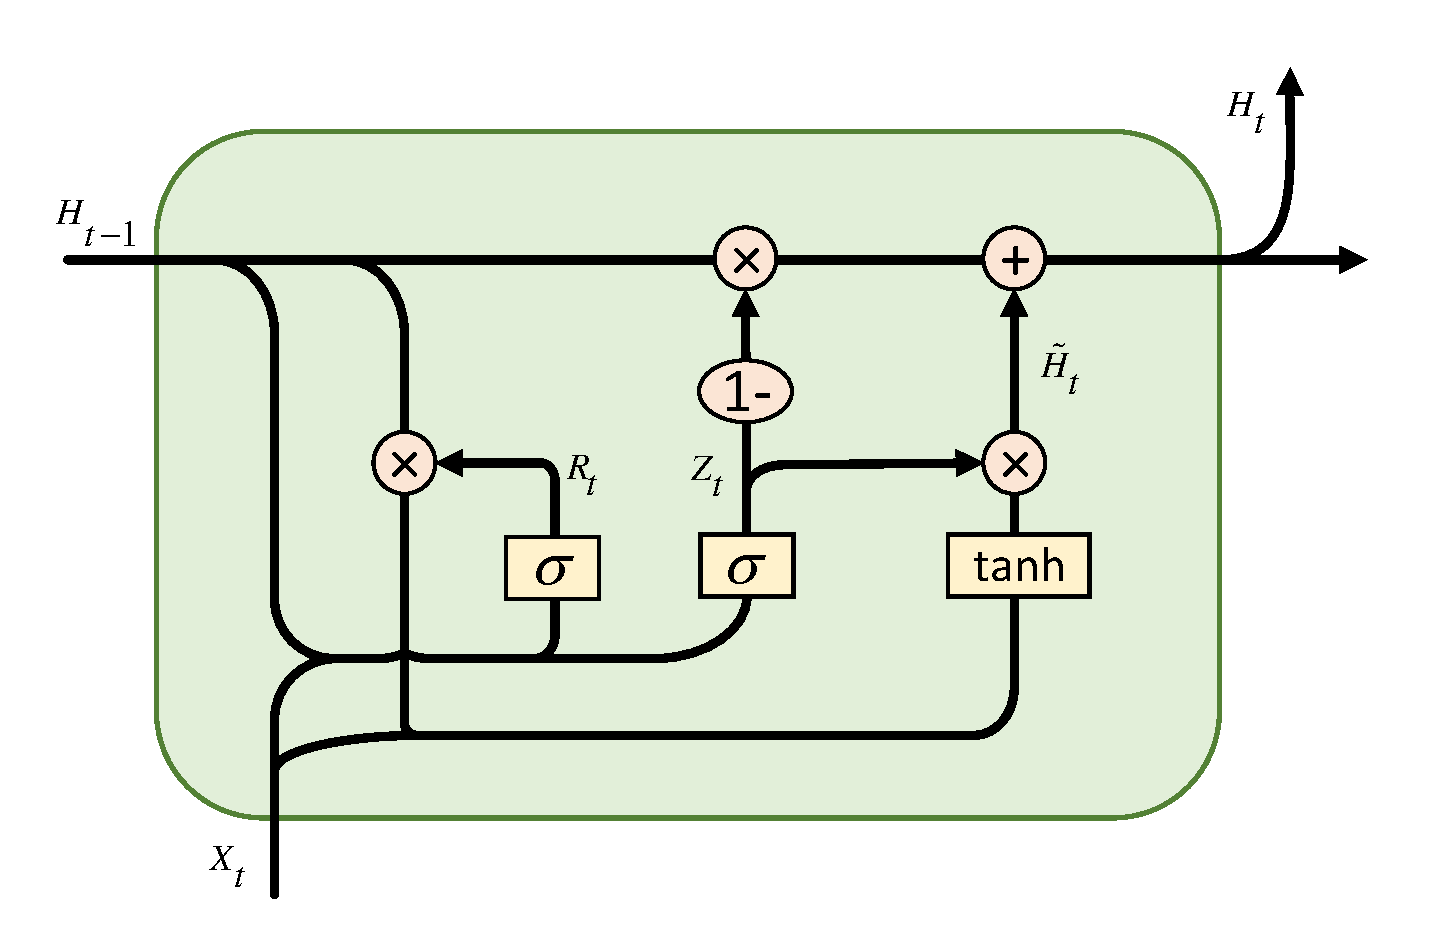
\includegraphics[width=0.7\textwidth]{./pic/gru.pdf}
\caption{标准GRU模型}
\label{Figure.3.2}
\end{figure*}

GRU模型是LSTM模型的一个变种,继承了LSTM模型能够学习序列数据中长期依赖性的特性。GRU相较于LSTM模型结构更加精简,并且在大多数任务上效果出色。由于GRU模型内部门控结构较少,在对时空特征进行融合时难度较大,但是GRU模型相较于LSTM存在天然的参数量上的优势。本章中的STGRU模型通过扩展GRU模型实现时空特征和地理结构特征的提取,并大幅降度了参数量。

标准的GRU模型如图\ref{Figure.3.2}所示,将LSTM中的遗忘门控和输入门控融合成一个更新门控,并去掉了单元状态,使用隐藏状态来传递信息。GRU的门控更新公式如下:
\begin{equation}
   R_t = \sigma(W_{xr}[H_{t-1},X_t]+b_r)
\end{equation}
\begin{equation}
   Z_t = \sigma(W_{xz}[H_{t-1},X_t]+b_z)
\end{equation}
\begin{equation}
   \tilde{H_t} = \tanh(W_{xh}X_t + W_{hh}(R_t \odot H_{t-1})+b_h)
\label{eq.3.1}
\end{equation}
\begin{equation}
  H_t = Z_t\odot H_{t-1}+(1-Z_t)\odot \tilde{H_t}
\label{eq.3.2}
\end{equation}

其中隐藏单元数量为$h$,在给定时间步$t$时,输入为$X_t\in \mathbb{R}^{n\times d}$,$d$表示批量大小,上一时间步的隐藏状态为$H_{t-1}$。$R_t,Z_t \in \mathbb{R}^{n\times h}$表示重置门控和更新门控,其中$\sigma(\cdot)$是$Sigmoid$函数。$\tilde{H_t}\in \mathbb{R}^{n\times h}$表示时间步$t$时的隐藏状态,其中$\tanh(\cdot)$是双曲正切函数。$W_{xr},W_{xz},W_{xh},W_{hr},W_{hz},W_{hh} \in \mathbb{R}^{d\times h}$则是各个门控的权重参数,$b_r,b_z,b_h$是对应的偏置向量。$\odot$表示矩阵的哈达玛积。

\subsection{时空门控循环单元}

\begin{figure*}[!ht]
\centering 
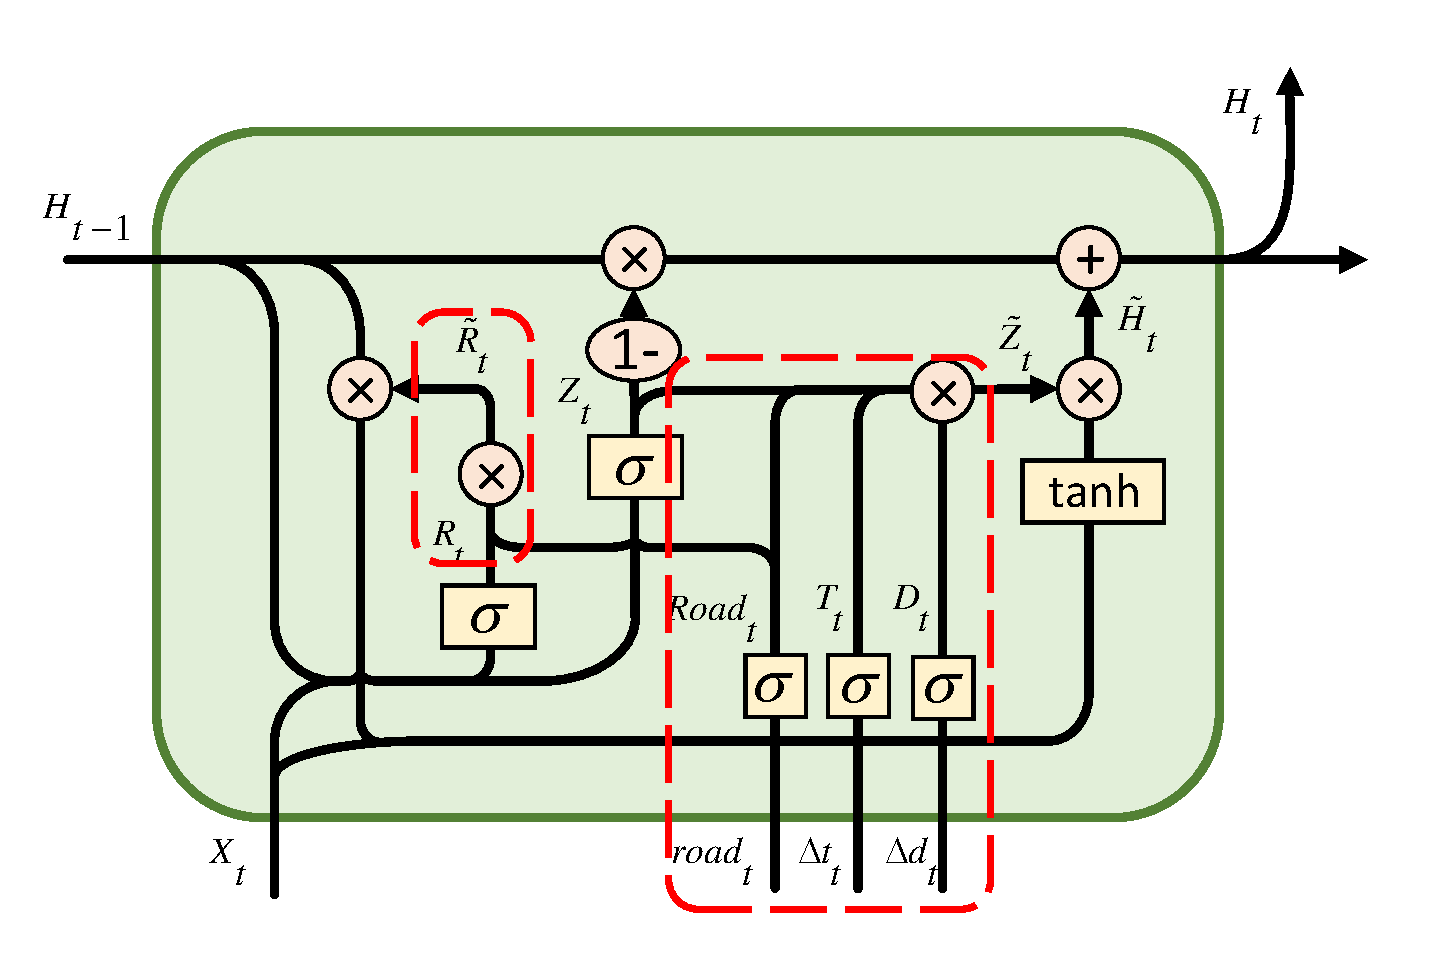
\includegraphics[width=0.7\textwidth]{./pic/stgru_add_box.pdf}
\caption{STGRU模型}
\label{Figure.3.3}
\end{figure*}

如图\ref{Figure.3.3}中的两个红色虚线框所示,STGRU增加了时间门控、距离门控和路网门,分别表示为$T_t$、$D_t$和$Road_t$。$T_t$、$D_t$分别用于建模时间间隔和距离间隔对轨迹预测的影响,$Road_t$用于捕获路网信息对行为模式的影响。STGRU是基于GUR进行扩展的,因此上述三个门控的计算公式也与GRU中的重置门控和更新门控类似,如下所示:
\begin{equation}
  T_t=\sigma(W_{xt}X_t+\sigma(\Delta t_tW_t)+b_t)
\end{equation}
\begin{equation}
  D_t=\sigma(W_{xd}X_t+\sigma(\Delta d_tW_d)+b_d)
\end{equation}
\begin{equation}
  Road_t=\sigma(W_{xroad}X_t+\sigma(road_tW_{road})+b_{road})
\end{equation}

为了利用$T_t$、$D_t$和$Road_t$三个门控捕获的特征信息,需要将其与重置门控和更新门控进行融合,修改后的计算公式为:
\begin{equation}
  \tilde{R_t} = R_t \odot Road_t
\end{equation}
\begin{equation}
  \tilde{Z_t} = Z_t \odot T_t \odot D_t \odot Road_t
\end{equation}

对应的公式\ref{eq.3.1}和\ref{eq.3.2}修改为:
\begin{equation}
  \tilde{H_t} = \tanh(W_{xh}X_t + W_{hh}(\tilde{R_t} \odot H_{t-1})+b_h)
\label{eq.3.3}
\end{equation}
\begin{equation}
  H_t = \tilde{Z_t}\odot H_{t-1}+(1-\tilde{Z_t})\odot \tilde{H_t}
\label{eq.3.4}
\end{equation}

其中$\Delta t_t$表示时间间隔,$\Delta d_t$表示距离间隔,$r_t$表示路网信息。$T_t$相当于输入信息中时间间隔特征的捕获器,$D_t$则为输入信息中距离间隔特征的捕获器,$Road_t$用于捕获输入信息中的路网结构特征。通过增加一个新重置门控状态$\tilde{R_t}$和新的更新门控状态$\tilde{Z_t}$用以计算路网门控对重置门控的影响以及三个门控同时对更新门控的影响。上述所有修改,共同确定新的隐藏状态$H_t$。

候选的隐藏状态$\tilde{H_t}$是由输入信息、重置门控和前一个时间步的隐藏状态决定的。重置门控的新状态$\tilde{R_t}$被设计用来记忆用户的长期路网访问信息。计算方式为先由$Road_t$记忆路网信息$r_t$,然后与输入信息一起融入$\tilde{R_t}$,再进一步融合到$\tilde{H_t}$。

标准GRU中的更新门控$Z_t$可以捕获短期依赖性,因此,设计了一个时间门控和距离门控,结合上述路网门控来控制更新门控的状态。$T_t$用于记忆轨迹点之间的时间间隔$\Delta t_t$,并参考LSTM中,使用逐元素相乘的哈达玛积将其融入新的更新门控状态$\tilde{Z_t}$中。同样的,$D_t$用于记忆轨迹点之间的距离间隔$\Delta d_t$,$Road_t$记忆路网信息,并均与$Z_t$通过哈达玛积得到$\tilde{Z_t}$。上述对于距离间隔以及时间间隔的建模可以帮助捕获用户的行为模式,如当前的移动速度、所处状态等。对路网信息的建模可以帮助捕获用户的短期行为约束和长期的目标,以及捕获用户之间的空间关系,这部分内容会在下一章中详细阐述。

根据上述模型结构,对于轨迹数据需要进行一定的处理。首先,需要计算轨迹点之间的时间间隔和距离间隔,于是$H^u$可以转化为:
\begin{equation}
\begin{split}
  [(r^u_1,0,0),(r^u_2,t^u_2-t^u_1,d (l_1,l_2)),\dots,
  (r^u_n,t^u_n-t^u_{n-1},d(l_{n-1},l_n))]
\end{split}
\end{equation}

然后,增加天气、假期信息和路网信息,并进一步处理为:
\begin{equation}
(r^u_n,weather_n,date_n,t^u_n-t^u_{n-1},d(l_{n-1},l_n),road_n)
\end{equation}

其中$r^u_t$包含经纬度信息和所在区域信息,$weather_t$则包括了最高温度、最低温度和平均温度,$date_t$根据轨迹点所属日期判断是否为节假日,用0,1区分标记。于是STGRU中的$X_t$就等价于$(r^u_t,weather_t,date_t)$,$\Delta t_t$由$t^u_t-t^u_{t-1}$计算得到,$\Delta d_t$则是两个轨迹点之间的距离间隔$d(l_{t-1}, l_{t})$,$d(\cdot,\cdot)$是欧式距离的计算公式。而$road_t$是一个向量,由轨迹点所在的道路节点以及其相邻节点编号拼接而成,节点编号为公开地图OpenStreetMap中对应路段的编号。例如,轨迹点$i$所处的道路节点为$node_i$,$node_i$的$c$邻居节点分别表示为$node_{i+1},node_{i+2},\dots,node_{i+c}$,那么$road_t$就可以表示为:
\begin{equation}
road_t = (node_{i},node_{i+1},\dots,node_{i+c})
\end{equation}

\begin{figure*}[!ht]
\centering
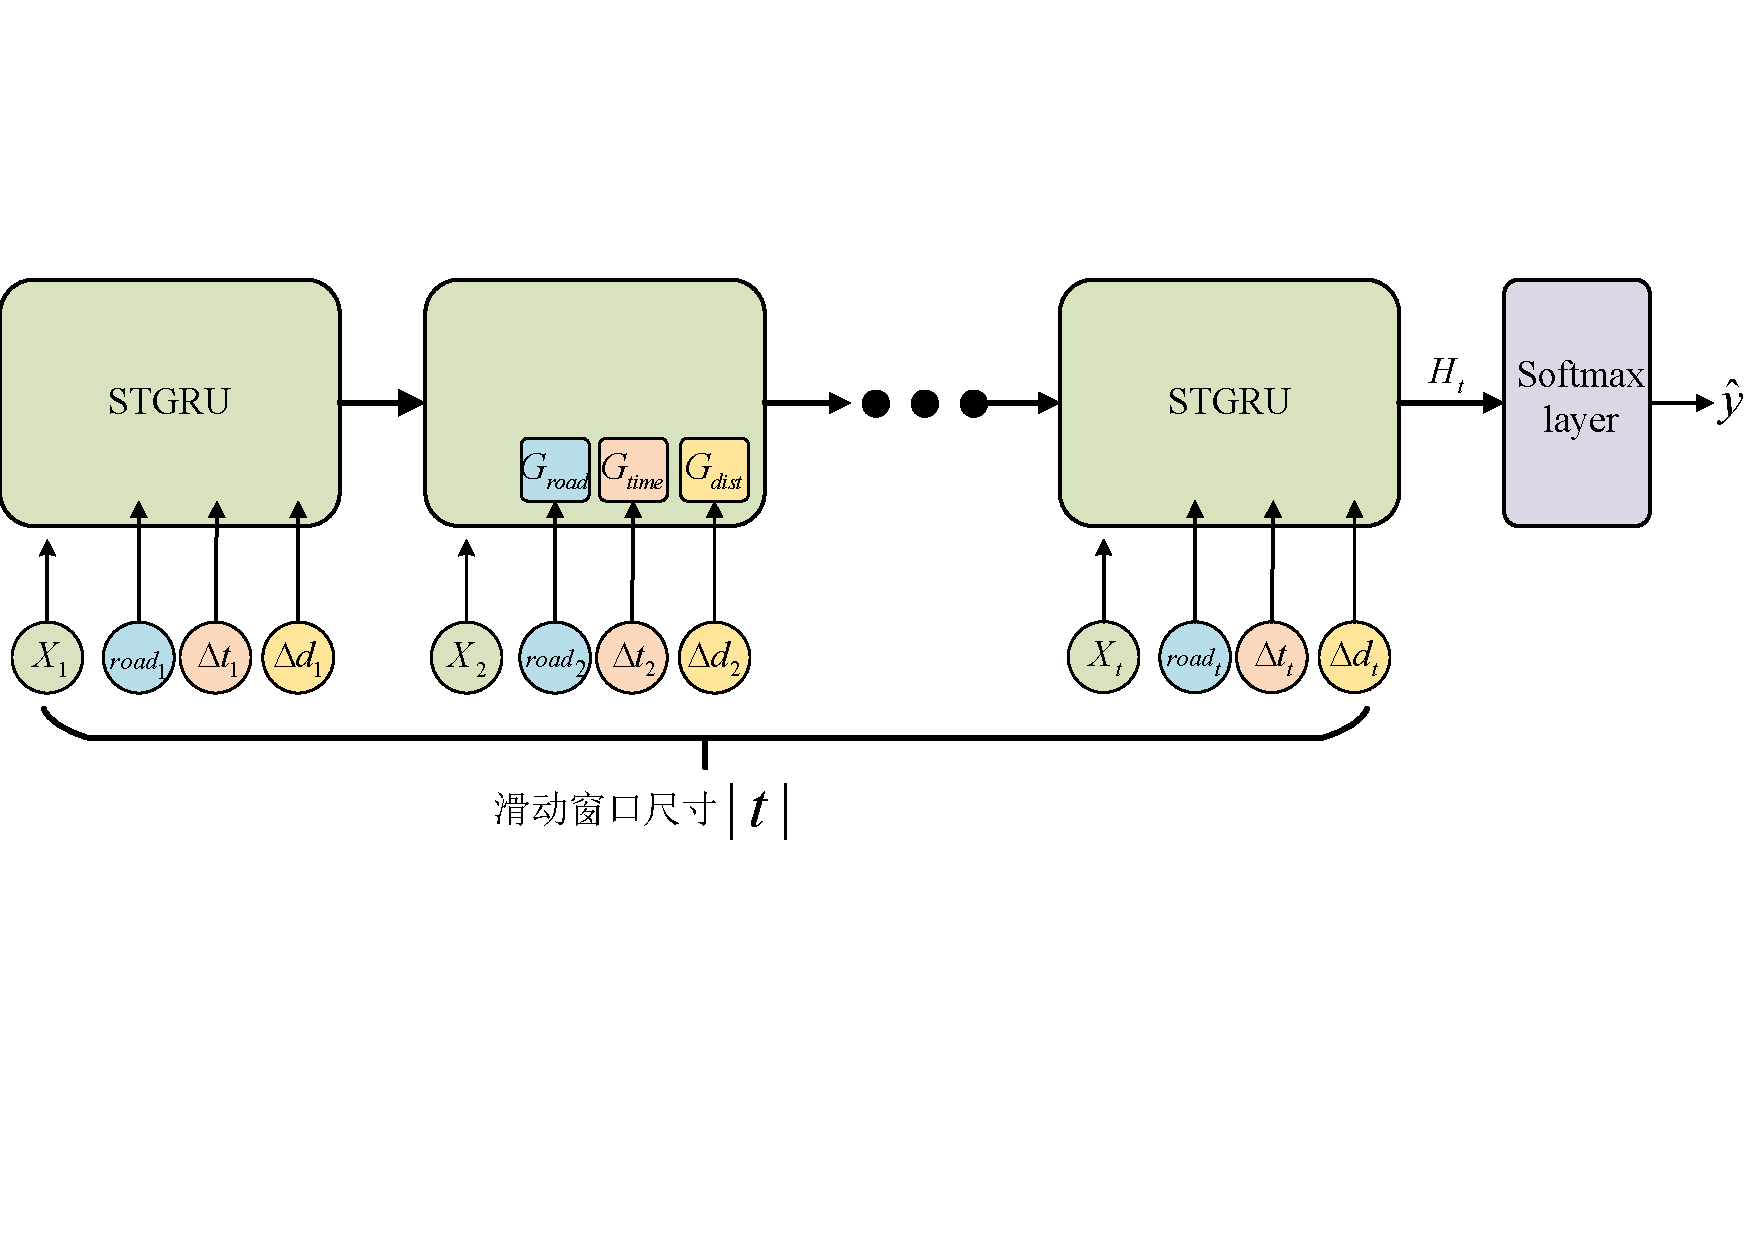
\includegraphics[width=1.0\linewidth]{./pic/stgru_all_4.pdf}
\caption{基于STGRU的轨迹预测模型}
\label{Figure.3.1}
\end{figure*}

如图\ref{Figure.3.1}所示,轨迹预测任务整体的模型架构通过堆叠一个STGRU层和一个softmax层得到,目的是为了减少对比实验的公平性,减少其他因素的影响。采用单层网络模型进行对比实验,以softmax作为分类器得到输出结果,使用多分类交叉熵作为损失函数:
\begin{equation}
J = -\sum_{i=1}^{K}y_i\log (p_i)
\end{equation}

\subsection{模型分析与训练}
STGRU模型相较于最新的时空特征模型,在一定程度上减少了模型参数的规模。单个STGRU单元的参数了可以计算为$3 \times d_h^2+6 \times d_h \times d_x+6 \times d_h$,其中$d_n$是隐藏单元数,$d_x$是输入的维度。同理,一个LSTM单元的参数量计算可得为$4 \times d_h^2+4 \times d_h \times d_x+4 \times d_h$。GRU单元相较于LSTM单元减少了一个门控结构,因此参数量也较少,为$3 \times d_h^2+3 \times d_h \times d_x+3 \times d_h$。本章中的基准模型STGN是目前通过扩展循环网络建模时空特征的模型中效果最好的,STGN基于LSTM进行了改进,参数量为$5 \times d_h^2+8 \times d_h \times d_x+10 \times d_h$。对比可以发现,STGRU模型的参数量不足STGN模型的三分之二。

在模型训练中,使用Adam优化器。Adam优化器同时考虑了一阶和二阶梯度,能够自动调整模型学习率,适用于大规模数据和参数量较大的场景。

\section{实验与分析}
本节首先对于本章的实验配置信息进行简单介绍。然后通过多组的对比实验、消融实验、应用分析,验证本章提出的STGRU模型在聚集预测场景轨迹预测任务上的有效性。

\subsection{实验配置和基线方法}
\label{实验配置}
本文所有实验所使用的实验环境如表\ref{Table.3.1}所示。
\begin{table*}[!ht]
\centering
\caption{实验环境配置表}%添加标题 设置标签
\label{Table.3.1}
\begin{tabular}{cl}
\toprule[1.5pt]
软硬件& 配置\\
\midrule[0.75pt]
CPU& Intel(R) Core(TM) i5-8600K CPU @ 3.60GHz\\
内存& 32GB DDR4\\
GPU&  GeForce RTX™ 2080 Ti $\times$ 2\\
GPU显存& 11GB GDDR6\\
操作系统& Ubuntu 16.04\\
Cuda版本& 11.4\\
cuDNN版本& V10.1.243\\
anaconda版本& 4.5.11\\
python版本& 3.6.3\\
tensorflow版本& 2.1.0\\
\bottomrule[1.5pt]
\end{tabular}
\end{table*}

本章实验基于章节2.3中所介绍的三个数据集展开。首先剔除了三个数据集中轨迹长度小于30的用户数据,然后将剩余数据的70$\%$作为训练集,20$\%$作为验证集,10$\%$作为测试集。

由于三个数据集中均不包含轨迹点对应的区域信息,仅包含较为稀疏的POI信息。因此以$1km$为边长对所拥有覆盖区域进行了划分,每个区域面积为$5km \times 5km$,并以常规的蛇形编号方式对区域进行编号。对于数据集中的轨迹点信息,通过经纬度计算对应的区域,增加相应的区域标签。在所有数据集上均采用滑动窗口的方法生成样本。由于数据集本身质量较高,采样间隔较短,为了模拟现实场景下处于隐私保护考虑、设备精度不足等问题导致的轨迹点缺失问题,在滑动窗口内部增加了随机采样机制,即生成样本时每个轨迹点之间的时间间隔并不均匀,而是随机决定的,目的是增加轨迹的复杂性,更符合现实场景。例如,生成样本时第一个轨迹点的时刻为上午8:00,随机区间为$[1-6]$。假设生成的随机数为3,样本的第二个轨迹点和第一个轨迹点之间的采样间隔为$3\times 5min=15min$,即为上午8:15。

本章选取了五种具有代表性的轨迹预测模型与STGRU进行对比实验,模型的详细介绍如下:
\begin{itemize}
\item[$\bullet$] \textbf{循环神经网络RNN}\citing{DBLP:conf/interspeech/MikolovKBCK10}: 循环神经网络在内部循环传递状态,因此适用于广义上的时间序列模型,并被广泛应用于各类时间序列预测任务中。

\item[$\bullet$] \textbf{长短时记忆网络LSTM}\citing{DBLP:journals/neco/HochreiterS97}: LSTM在大幅缓解了RNN存在的梯度消失和梯度爆炸问题,适用于处理和预测时间序列中时间跨度较长的事件。

\item[$\bullet$] \textbf{门控循环单元GRU}\citing{DBLP:conf/emnlp/ChoMGBBSB14}: GRU是LSTM模型的一个变种,参数量上比LSTM略少,性能上与LSTM相近,某些小数据集上甚至表现出更好的性能。

\item[$\bullet$] \textbf{分层时空长短时记忆网络HST-LSTM}\citing{DBLP:conf/ijcai/Kong018}: HST-LSTM尝试将时空影响融合到LSTM的三个门控中,使用LSTM本身结构来尝试提取时空特征。由于本章使用的数据集中并没有会话信息,因此采用其通用版本ST-LSTM进行对比实验。

\item[$\bullet$] \textbf{时空门控记忆网络STGN}\citing{DBLP:conf/aaai/ZhaoZLXLZSZ19}: 通过增强LSTM结构,引入两对时空门空结构来捕获时空关系,是目前性能最好的模型之一。
\end{itemize}

\subsection{评价指标}
为了评估STGRU模型的性能,并与上述五个基线方法进行比较,本章使用AUC和Recall@k两个指标作为评价标准。基于区域的轨迹预测任务本质上是一个多分类任务,AUC指标可以较好地评估模型分类效果,具体原理见第二章。Recall@k则是正确预测数与总预测数的比例。在本章中,使用$K=\{1,5,10,15,20\}$来计算Recall@K的不同结果。多分类交叉熵得到的结果是对应每个区域一个概率,所有区域的概率和为1。对所有区域按照其概率从高到低排列。recall分数计算为概率最大的前K个区域中发现真实区域的次数的百分比。$U$是用户集合,假设$L_u$代表测试数据中用户$u$的真实区域集合,$P_{K,u}$表示前K个预测区域的集合,则Recall@K的计算公式可以表示为:
\begin{equation}
Recall@K = \frac{1}{|U|} \sum_{u\in U}\frac{|L_u\cap P_{K,u}|}{|L_u|}
\end{equation}

\subsection{对比实验}
\label{对比实验设置}
\textbf{方法比较。}表\ref{Table.3.2}中给出了STGRU模型和六个基线模型在三个数据集上通过Recall@K和AUC评估的性能。在所有对比实验中,隐藏状态的大小设置为32,迭代次数设置为200,批量大小设置为512,滑动窗口大小设置为10,名古屋人流数据集和大阪人流数据集的随机时间间隔为1到3,东京人流数据集的随机时间间隔为1到5,原因是东京人流数据集中的数据密度更高,通过增加随机时间间隔可以提高数据的复杂性,后续对与不同随机时间间隔也进行了对比实验,验证随机时间间隔大小对实验的影响。本章的所有实验都使用相同的参数设置。
\begin{table*}[!ht]
\centering
\caption{在三个数据集上Recall@K和AUC指标的结果}%添加标题 设置标签
\label{Table.3.2}
\setlength{\tabcolsep}{5mm}{
\begin{tabular}{cccccc}% 通过添加 | 来表示是否需要绘制竖线
\toprule[1.5pt]  % 在表格最上方绘制横线
\textbf{NPF}  & recall@1 & recall@5 & recall@10 & recall@20 & AUC\\
\midrule[0.75pt]
LSTM    & 0.0428   & 0.1677   & 0.2894    & 0.4300    & 0.6951 \\

GRU     & 0.0712   & 0.2372   & 0.3421    & 0.4771    & 0.7778 \\

RNN     & 0.0809   & 0.2580   & 0.3570    & 0.4865    & 0.8018 \\

ST-LSTM & 0.0621   & 0.2438   & 0.3663    & 0.5050    & 0.7976 \\

STGN    & 0.0762   & 0.2728   & 0.3734    & 0.5061    & 0.8177 \\

STGRU   & \textbf{0.0920}   & \textbf{0.2829}   & \textbf{0.3891}    & \textbf{0.5231}    & \textbf{0.8290} \\
\bottomrule[1.5pt] % 在表格最下方绘制横线
\end{tabular}
\\
\centering
\begin{tabular}{cccccc}% 通过添加 | 来表示是否需要绘制竖线
\toprule[1.5pt]  % 在表格最上方绘制横线
\textbf{OPF}  & recall@1 & recall@5 & recall@10 & recall@20 & AUC\\
\midrule[0.75pt]
LSTM    & 0.0383 & 0.1638 & 0.2634 & 0.4375 & 0.7140 \\

GRU     & 0.0455 & 0.1979 & 0.3007 & 0.4656 & 0.7611 \\

RNN     & 0.0588 & 0.2258 & 0.3260 & 0.4881 & 0.8324 \\

ST-LSTM & 0.0502 & 0.2107 & 0.3174 & 0.4890 & 0.7817 \\

STGN    & 0.0633 & 0.1699 & 0.2833 & 0.4920 & 0.8292 \\

STGRU   & \textbf{0.0681} & \textbf{0.2439} & \textbf{0.3464} & \textbf{0.5116} & \textbf{0.8545} \\
\bottomrule[1.5pt] % 在表格最下方绘制横线
\end{tabular}
\\
\centering
\begin{tabular}{cccccc}% 通过添加 | 来表示是否需要绘制竖线
\toprule[1.5pt]  % 在表格最上方绘制横线
\textbf{TPF}  & recall@1 & recall@5 & recall@10 & recall@20 & AUC\\
\midrule[0.75pt]
LSTM    & 0.0752 & 0.3331 & 0.4849 & 0.6428 & 0.8317 \\

GRU     & 0.0789 & 0.3319 & 0.4793 & 0.6384 & 0.8451 \\

RNN     & 0.0856 & 0.3634 & 0.5066 & 0.6561 & 0.8645 \\

ST-LSTM & 0.0864 & 0.3699 & 0.5213 & 0.6682 & 0.8727 \\

STGN    & 0.0900 & 0.3327 & 0.5103 & 0.6672 & 0.8734 \\

STGRU   & \textbf{0.0933} & \textbf{0.3795} & \textbf{0.5263} & \textbf{0.6730} & \textbf{0.8755} \\
\bottomrule[1.5pt] % 在表格最下方绘制横线
\end{tabular}}
\end{table*}

如表中实验结果所示,本章提出的STGRU模型在三个数据集的所有指标上都明显优于现有的最先进方法STGN。在名古屋、大阪和东京数据集的$Recall@1$指标上,STGRU模型相较于五个基线模型的性能提升分别为18.1$\%$ - 110.2$\%$,5.7$\%$ - 74.7$\%$和3.7$\%$ - 24.1$\%$。同时在其他$Recall@k$指标上相较于最新的STGN模型最大提升比例分别达到了43.5$\%$,22.3$\%$和3.9$\%$。结果表明,STGRU模型中对于路网结构特征提取的机制可以更好地建模用户行为模式,对短期时空上下文特征的建模提升了在强实时数据下的效果,以及对轨迹预测的任务有效性。这是因为添加的路网门控与更新门控相结合,将短期路网特征融合到模型中,而重置门控则与长期路网特征相结合。

此外,RNN模型在这三个数据集上的表现比LSTM模型略好。这是因为RNN模型具有短期记忆的特点。时间越近,轨迹点的权重就越大。因此即使加入了随机区间,得到的样本仍然具有较强的实时性,所以RNN模型的性能更好。同样,GRU模型在对强实时数据进行建模时也优于LSTM模型。HST-LSTM模型和STGN模型的性能优于以上三种模型,这验证了时空特征对轨迹预测的重要性。其中,STGN模型的性能优于HST-LSTM模型,验证了通过特定门控结构提取时空特征的方式比在LSTM门控基础上的融合改进更为有效,其原因可能是参数的增加带来的模型建模能力的提升。

在进行对比实验的三个数据集中,每个数据集涵盖了日本一个地区总共6天的轨迹数据,相邻轨迹点之间的时间间隔为5分钟,因此时间上的刻度总数为$6\times 24 \times 60 \div 5 = 1728$。数据集所对应的每个地区可分为约5000至10000个区域。以NPF数据集为例,区域的数量约为5000。计算可以得到,该数据集的时空矩阵大小约为$5000\times 2000$。然而,NPF数据集中的轨迹点的数量只有100万。在去除重复的时空区域后,轨迹点覆盖矩阵的大小小于数据集的时空矩阵大小的1$\%$。RNN、LSTM和GRU等模型直接对时空矩阵进行训练,这将导致严重的数据稀疏问题。STGRU模型通过时间间隔、距离间隔和路网结构在轨道点之间增加约束。在训练STGRU模型时,只需要考虑每个样本所覆盖的局部区域以及轨迹点的周边区域,这大大缓解了数据集的数据稀少问题,与上述三个模型相比,可以更好地建模用户行为模式,有效的提升了模型对轨迹数据的预测性能。


\textbf{参数影响。}在标准的RNN模型中,不同的单元大小将导致不同的性能。于是进行了不同隐藏状态大小对STGRU模型性能的影响试验。通过改变隐藏状态大小为$32,64,128,256,512$来比较不同隐藏状态大小对STGRU模型性能的影响。从表\ref{Table.3.3}可以看出,在一定程度上增加隐藏状态尺寸可以提高STGRU模型的性能。但是过大的隐藏状态尺寸会增加训练时间,导致性能下降。当模型的单元数量确定后,隐藏状态大小决定了模型的复杂性,适当地增大隐藏状态尺寸能够更好地拟合数据,得到更好的性能表现。
\begin{table}[ht]
\centering
\caption{STGRU模型在不同隐藏状态大小下的性能}
\label{Table.3.3}
\setlength{\tabcolsep}{1mm}{
\begin{tabular}{ccccc}% 通过添加 | 来表示是否需要绘制竖线
\toprule[1.5pt]  % 在表格最上方绘制横线
\textbf{cell size}  & recall@1 & recall@5 & recall@10 & recall@20 \\
\midrule[0.75pt]
32    & 0.0933 & 0.3795 & \textbf{0.5263} & 0.6730\\

64     & 0.0922 & \textbf{0.3836} & 0.5253 & \textbf{0.6754}\\

128     & \textbf{0.0942} & 0.3774 & 0.5217 & 0.6736 \\

256 &   0.0923 &  0.3761  &  0.5238   & 0.6704 \\
 % 在表格最下方绘制横线
512 &   0.0913 & 0.3760   &   0.5190  &  0.6658\\
\bottomrule[1.5pt]
\end{tabular}}
\end{table}

\subsection{消融实验}
\textbf{时间门控和距离门控的有效性。}STGRU使用了一个时间门控和一个距离门控与更新门控相结合来捕获短期的依赖关系。时间门控和距离门控对建模时间间隔和距离间隔的有效性是很重要的。如公式\ref{eq.3.4}所示,时间门控和距离门控可以通过设置$T_t=1$和$D_t=1$来关闭。同时为了消除路网门控的干扰,STGRU模型中的路网门控也被关闭。因此在名古屋人流数据集上进行了三组实验,分别为关闭时间门控、关闭距离门控和同时关闭两个门控,以比较和验证时间门控和距离门控的有效性。
\begin{table}[ht]
\caption{时间门控和距离门控对模型性能的影响}
\label{Table.3.4}
\centering
\setlength{\tabcolsep}{1mm}{
\begin{tabular}{ccccc}% 通过添加 | 来表示是否需要绘制竖线
\toprule[1.5pt]  % 在表格最上方绘制横线
\textbf{NPF}  & recall@1 & recall@5 & recall@10 & recall@20 \\
\midrule[0.75pt]
GRU    & 0.0712 & 0.2372 & 0.3421 & 0.4771\\

GRU+$D_t$     & 0.0887 & 0.2763 & 0.3778 & 0.5080 \\

GRU+$T_t$     & 0.0844 & 0.2744 & 0.3773 & 0.5099 \\

GRU+$D_t+T_t$ & \textbf{0.0909} & \textbf{0.2801} & \textbf{0.3805} & \textbf{0.5116} \\
\bottomrule[1.5pt] % 在表格最下方绘制横线
\end{tabular}}
\end{table}

从表\ref{Table.3.4}中可以发现,时间门控和距离门控在实验数据集上的重要性相似。与GRU模型相比,同时增加时间门控和距离门控的$GRU+D_t+T_t$在四个评价指标上的性能提升分别为27.67$\%$、18.04$\%$、11.22$\%$和7.23$\%$。而仅增加一个门控结构的$GRU+T_t$和$GRU+D_t$之间性能差异非常小,说明距离间隔和时间间隔对行为模式的建模有类似的效果。而且,$GRU+D_t+T_t$相较于$GRU+T_t$和$GRU+D_t$的性能提升很小,说明在测试数据集上,时间间隔和距离间隔的特征存在很大程度的重叠。

\textbf{路网门控的有效性。}在STGRU中设计了一个路网门控,它与更新门控和重置门控结合在一起,以捕捉长期和短期的路网依赖性。本组实验的动机是通过实验研究路网门控在更新门控和复位门控中的作用。如公式\ref{eq.3.3}和\ref{eq.3.4}所示,在$\tilde{R_t}$和$\tilde{Z_t}$中分别设置$Road_t = 1$,即可以关闭路网门控。通过设置在名古屋人流数据集上的三组实验,即关闭所有路网门控和分别关闭单个路网门控,以验证路网闸门在捕捉长期和短期依赖关系方面的有效性。
\begin{table}[ht]
\centering
\caption{路网门控对模型性能的影响}
\label{Table.3.5}
\setlength{\tabcolsep}{1mm}{
\begin{tabular}{ccccc}% 通过添加 | 来表示是否需要绘制竖线
\toprule[1.5pt]  % 在表格最上方绘制横线
\textbf{NPF}  & recall@1 & recall@5 & recall@10 & recall@20 \\
\midrule[0.75pt]
STGRU-$R_t$    & 0.0909 & 0.2801 & 0.3805 & 0.5116\\

STGRU-$R_{2t}$     & 0.0867 & 0.2776 & 0.3786 & 0.5101 \\

STGRU-$R_{1t}$     & 0.0862 & 0.2795 & 0.3796 & 0.5093 \\

STGRU & \textbf{0.0920}   & \textbf{0.2829}   & \textbf{0.3891}    & \textbf{0.5231} \\
\bottomrule[1.5pt] % 在表格最下方绘制横线
\end{tabular}}
\end{table}

如表\ref{Table.3.5}所示,关闭单个路网门控的性能不如关闭所有路网门控。这可能是由于路网结构的长期特征和短期特征需要一起使用。
关闭单个路网门控会导致路网信息对预测结果无效。同时,一些参数会被用来对路网特征进行建模,这一原因导致了模型的性能下降。因此,单独关闭一个路网门控的性能几乎是一样的。

\textbf{滑动窗口大小的影响。}在上述对比实验中,训练样本和测试样本均是通过滑动窗口采样取得。滑动窗口的大小限制了单个样本的长度。为了比较STGRU模型在不同大小的滑动窗口中的性能,通过设置不同尺寸的滑动窗口来获取不同长度样本进行实验,分别为10、15、20、25和30。为了保证较大滑动窗口尺寸下的样本数量,在东京人流数据集上进行实验,因为该数据集的平均轨迹长度最长。
\begin{table}[ht]
\centering
\caption{不同长度滑动窗口对模型性能的影响}
\label{Table.3.6}
\setlength{\tabcolsep}{1mm}{
\begin{tabular}{ccccc}% 通过添加 | 来表示是否需要绘制竖线
\toprule[1.5pt]  % 在表格最上方绘制横线
\textbf{Window Size}  & recall@1 & recall@5 & recall@10 & recall@20 \\
\midrule[0.75pt]
10    & 0.0933 & 0.3795 & 0.5263 & 0.6730\\

15     & 0.0929 & \textbf{0.3897} & 0.5331 & 0.6828 \\

20     & 0.0949 & 0.3624 & 0.5174 & 0.6786 \\

25 & 0.0905   & 0.3794   & 0.5267    & 0.6831 \\
 % 在表格最下方绘制横线
30 & \textbf{0.1014}   & 0.3611   & \textbf{0.5842}    & \textbf{0.6957} \\
\bottomrule[1.5pt]
\end{tabular}}
\end{table}

样本长度决定了模型的单元数量,以及模型的参数。如表\ref{Table.3.6}所示,随着滑动窗口长度的增加模型参数量会同比增加,模型的整体性能有一定的提高。当滑动窗口大小为30时,模型参数量是滑动窗口大小为10时的3倍,四个指标的性能提升分别为8.68$\%$、-4.85$\%$、11$\%$和3.37$\%$。虽然样本长度的增加可以提高模型的性能,但出于聚集预测任务的实际应用场景考虑,样本长度在10以内更有意义,这也是在与基线模型进行对比实验时滑动窗口大小设置为10的主要原因。

\textbf{随机区间大小的影响。}另一个重要参数是滑动窗口中随机区间的大小。通过对滑动窗口中的轨迹点之间的时间间隔进行随机采样,目的是提高轨迹样本的复杂性。为了比较不同的随机区间对轨迹样本的复杂性和模型性能的影响,在东京人流数据集上设置了不同的随机区间进行对比实验,分别为3、5、7、9、11。选择东京人流数据集是因为该数据集的轨迹密度较大,轨迹点之间的连续性很强,需要增加一定的复杂性才更符合实际应用场景下的轨迹数据分布。
\begin{table}[ht]
\centering
\caption{不同随机时间间隔对模型性能的影响}
\label{Table.3.7}
\setlength{\tabcolsep}{1mm}{
\begin{tabular}{ccccc}% 通过添加 | 来表示是否需要绘制竖线
\toprule[1.5pt]  % 在表格最上方绘制横线
\textbf{Rand Interval}  & recall@1 & recall@5 & recall@10 & recall@20 \\
\midrule[0.75pt]
3    & 0.0889 & 0.3725 & 0.5148 & 0.6636\\

5     & \textbf{0.0933} & 0.3795 & 0.5263 & 0.6730 \\

7     & 0.0920 & \textbf{0.3835} & \textbf{0.5300} & \textbf{0.6776} \\

9 & 0.0822   & 0.3677   & 0.5196    & 0.6752 \\
 % 在表格最下方绘制横线
11 & 0.0747   & 0.3512   & 0.5104    & 0.6702 \\
\bottomrule[1.5pt]
\end{tabular}}
\end{table}

由表\ref{Table.3.7},可以看出随机区间大小为5和7时,STGRU模型性能最好,随机区间大小过大和过小都会导致模型性能下降。在另外两个数据集上,随机区间大小为3时,模型性能较好,这就是在与基线模型的对比实验中三个数据集分别使用不同的随机区间的原因,使用随机区间可以使样本更接近于真实世界的数据。

\subsection{应用分析}
最后,为了验证STGRU模型能够有效处理和预测短轨迹数据和长轨迹数据,与基线模型进行了两组应用分析实验。
\begin{figure}[!ht]
\centering
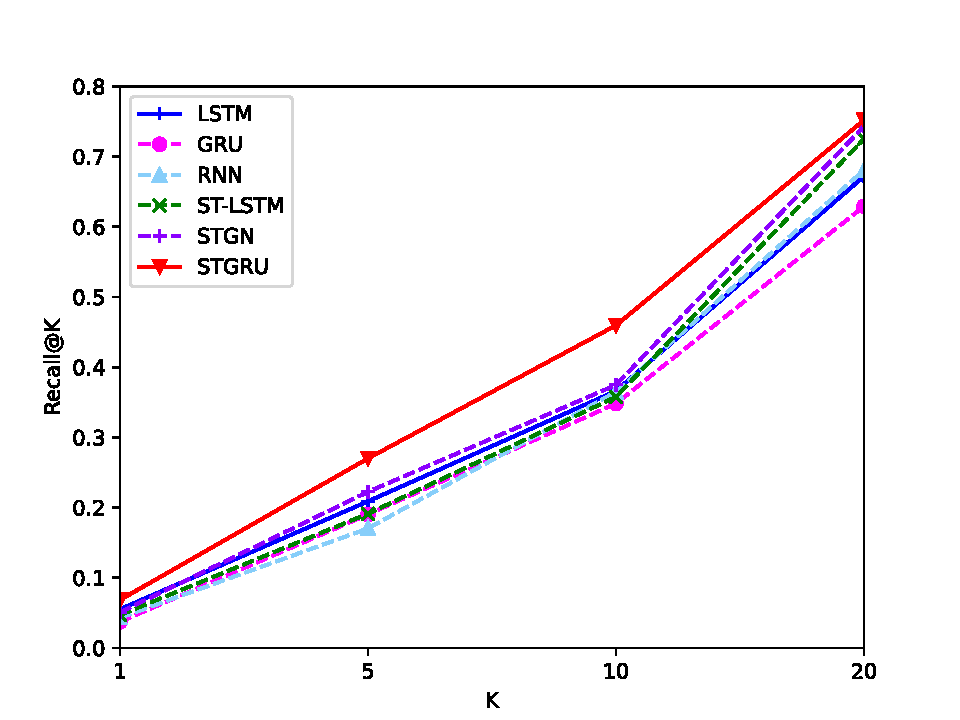
\includegraphics[scale=0.5]{./pic/f2.pdf}
\caption{STGRU模型在轨迹长度小于30的数据上的性能}
\label{Figure.3.4}
\end{figure}

如果用户的轨迹数据很稀少,就意味着很难理解用户的行为模式,这就对模型的性能要求更高,第一组实验基于东京人流数据集,在轨迹长度小于30的数据上进行实验,由于数据集过短没有使用随机间隔,使用最原始的滑动窗口生成样本,评价指标依旧为$recall@k$。如图\ref{Figure.3.4}所示,STGRU模型在recall@1和recall@5上的表现最好,这说明了STGRU模型能更好地处理稀疏数据。

\begin{figure}[!ht]
\centering
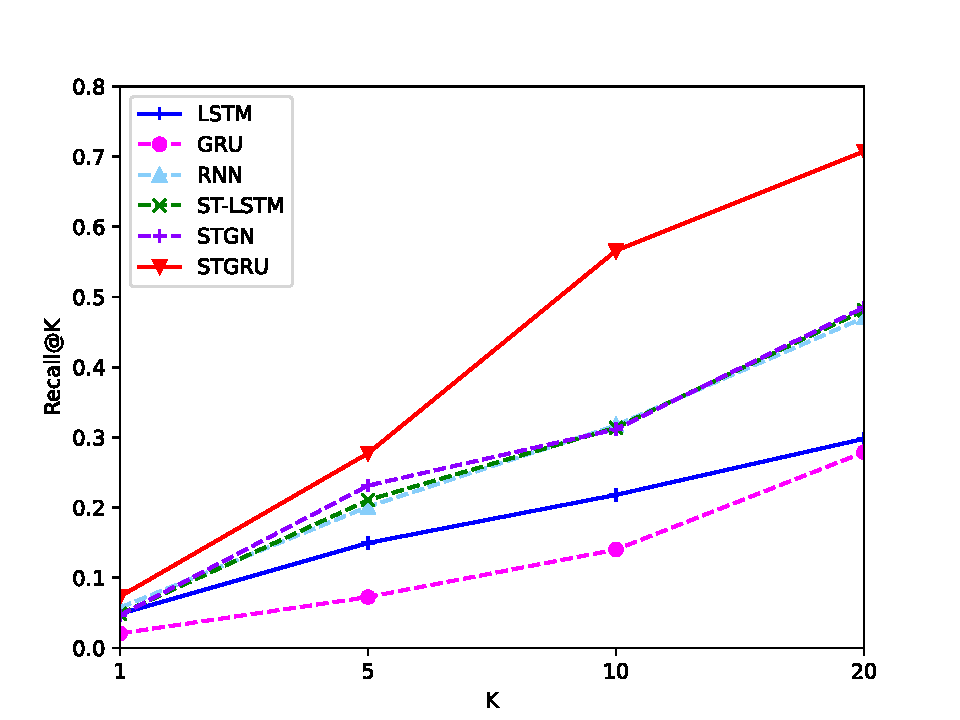
\includegraphics[scale=0.5]{./pic/f1.pdf}
\caption{STGRU模型在轨迹长度大于200的数据上的性能}
\label{Figure.3.5}
\end{figure}
在另一组实验中,使用的是轨迹长度大于200的数据,并沿用了对比实验中的参数设置。如图\ref{Figure.3.5}所示,在长轨迹数据上,STGRU模型的性能也优于所有基线模型,这验证了STGRU模型能够较好地提取和使用长期特征,特别是长期路网特征对强实时数据建模依然是有效的。


\section{本章小节}
在本章中,通过增强门控循环单元(GRU),提出了一个时空门控循环单元(STGRU)模型。在STGRU中,引入了时间门控和距离门控来捕获连续轨迹点之间的时间间隔和距离间隔特征,这对于建模用户的短期行为至关重要;然后引入了路网门控来捕获长期和短期路网结构。路网结构所代表的地理环境对用户的短期和长期行为都至关重要。上述三个门控结构与GRU中的更新门控相结合,用以建模用户的短期行为模式。只有路网门控与GRU中的重置门控相结合,建模用户的长期行为模式。并在三个真实世界的数据集上的实验结果验证了STGRU模型的有效性,它优于最新的方法。

\chapter{基于空间特征增强的聚集预测方法}
本章首先分析了轨迹预测方法在聚集预测任务下的局限性,并阐述解决问题的思路。然后详细介绍了本章所使用的希尔伯特曲线和图嵌入方式增强轨迹数据空间特征的原理。最后在真实世界的人流轨迹数据集上模拟现实场景下的聚集预测任务进行评估,并通过实验验证所提出模型的有效性。

\section{引言}
聚集预测能够对根据用户的历史轨迹信息及当前分布状态预测未来的用户位置,当前聚集预测算法通常对用户轨迹预测结果进行融合得到聚集预测结果,其主要难点如何建模在于同一时空下多轨迹之间关联特征。同时聚集预测任务对数据集要求较高,在用户数量和轨迹质量满足要求的前提下,还对数据的时空分布有所要求。但是现有方法主要针对单个用户的行为模式进行建模,忽略了用户之间的相互影响以及城市地理环境对用户行为模式的影响。

现有的轨迹预测方法通常使用用户时空特征和轨迹序列信息建模每个用户的行为模式,但并没有考虑用户之间的相互影响,如道路中的拥堵情况、多用户的趋同性等。目前只有交通流量预测对用户之间关联性的时空特征进行挖掘建模。交通流量预测对各个路段的流量进行分时段统计,再根据各路段之间的结构关系以及交通流量的变化模式进行建模,实现当前路段的流量预测。如时间图卷积网络(T-GCN)\citing{DBLP:journals/tits/ZhaoSZLWLDL20}对每个时间片按快照的形式进行输入,在时间维度上使用GRU模型进行建模的方式,以及时空图卷积网络(STGCN)\citing{DBLP:conf/ijcai/YuYZ18}在时间维度上使用单维卷积网络建模时间特征。

然而,聚集预测需要同时建模多用户轨迹\citing{DBLP:conf/sigir/LinNWL18}的时空特征和用户之间的关联特征。受上述两个模型的启发,历史的用户分布信息对多用户场景下特定用户的行为模式有较大影响。道路的拥堵情况,若当前部分可选择道路存在拥堵现象,其余可选道路的被选择概率就会上升。多用户的趋同性,大型活动的举办会吸引大量用户前往,其周围道路的流量将会出现持续的增长,此时周边某个用户以此地为目的地的概率也将大大增加。流量数据与道路结构信息都有利于建模多用户之间的行为模式。

为了建模同一时空下用户分布情况对行为模式影响以及进一步增强数据空间特征,本章提出了一种基于空间特征增强的聚集预测模型(Spatial Enhanced Gather Prediction Model,SEGPM)。通过引入希尔伯特扫描算法进行区域编号,增强了区域编号之间的空间特征。并设计了一种基于统计的路网图构建方式,将用户的分布信息和路网结构信息通过图嵌入得到,生成向量通过STGRU模型的路网门控进行建模。实验表明,考虑用户之间的相互影响和区域编号的空间特征增强能够有效提高模型性能。

本章主要工作总结如下:

(1)在轨迹区域的编号方式上引入希尔伯特扫描算法进行编号,可以增强标签之间的空间关联性。

(2)基于数据集统计信息构建以路段为节点的路网图,在STGRU中使用路网结构的嵌入表示建模同一时空下用户之间的关联特征和增强路网的结构特征。

(3)在三个真实世界数据集上评估了空间特征增强方法的有效性。

\section{基于空间特征增强的聚集预测模型}
本节首先给出了聚集预测的定义,并介绍了基于空间特征增强的聚集预测模型,然后介绍了希尔伯特曲线进以及基于希尔伯特扫描算法生成区域标签的方法,最后阐述了基于统计的路网图构建方法和使用的图嵌入方法。

\subsection{聚集预测问题定义及模型架构}
首先对聚集预测问题进行定义:

假设有$M$个用户的轨迹信息,用户的集合表示为$\mathbb{U}= \{u_1,u_2,\dots, u_M\}$,每个用户的轨迹信息表示为$Traj_u = \{(lat_1,lon_1,t_1), (lat_2,lon_2,t_2), \dots, (lat_n,lon_n,t_n)\}$,其中$n$为每个用户的轨迹长度。于是,用户$u$在当前时刻$t$之前的历史轨迹信息可以表示为$Ht_i^u = \{(lat_{t_1}^u,lon_{t_1}^u,t_1),(lat_{t_2}^u,lon_{t_2}^u,t_2), \dots, (lat_{t_{i-1}}^u,lon_{t_{i-1}}^u,t_{i-1})\}$。

区域划分方式为网格划分,所有区域的集合表示为$\mathcal{R}egion=\{r_1,r_2,\dots, r_{a^2}\}$,其中$r_i$表示对应区域编号。用户$u$在当前时刻$t$之前的历史访问信息可以表示为$Hr_i^u = \{r_{t_1}^u, r_{t_2}^u, \dots, r_{t_{i-1}}^u\}$,其中$r_{t_i}^u$表示用户$u$在$t_i$时刻所在的区域。

通过聚集预测模型预测用户$u$在$t_i$时刻所在的区域,输出结果为用户在所有区域的可能性向量$[s^u_{r_1,t_i},s^u_{r_2,t_i},\dots,s^u_{r_{a^2},t_i}]$。对于用户$u$,在$t_i$时刻出现在区域$r^{\prime}$的概率为对应的预测分数$s^u_{r^{\prime},t_i}$。

根据所有用户轨迹的预测结果,可以得到$M\times k$个用户分布的区域预测,其中$k$表示模型输出结果的前$k$个区域。对每个用户的前$k$各区域的预测结果进行归一化处理,保证每个用户的权重相等。用户$u$在$t_i$时刻可能出现在区域$r^{\prime}$中的概率为:
\begin{equation}
   \hat{s}^u_{r^{\prime},t_i} = \frac{s^u_{r^{\prime},t_i}}{\sum\limits_{j=0}^{k} s^u_{r_j,t_i}}
\end{equation}

于是可以计算区域$r^{\prime}$中在$t_i$时刻可能存在的人数$number_{r^{\prime},t_i}$。是否发生聚集则根据$number_{r^{\prime},t_i}$与阈值$\eta$的比较来判断。
\begin{equation}
   number_{r^{\prime},t_i} = \sum_{u\in U} \hat{s}^u_{r^{\prime},t_i}
\end{equation}
\begin{align}
    r^{\prime}_{state} &= 
        \begin{cases}
        1,& number_{r^{\prime},t_i}\ge \eta 
        \\
        0,& number_{r^{\prime},t_i}< \eta
        \end{cases}
\end{align}

其中$r^{\prime}_{state}$表示区域$r^{\prime}$是否发生聚集,$1$表示区域$r^{\prime}$发生聚集,$0$表示区域$r$没有发生聚集。$number_{r^{\prime},t_i}$则表示区域$r^{\prime}$中在$t_i$时刻可能存在的人数。

\begin{figure*}[!ht]
\centering
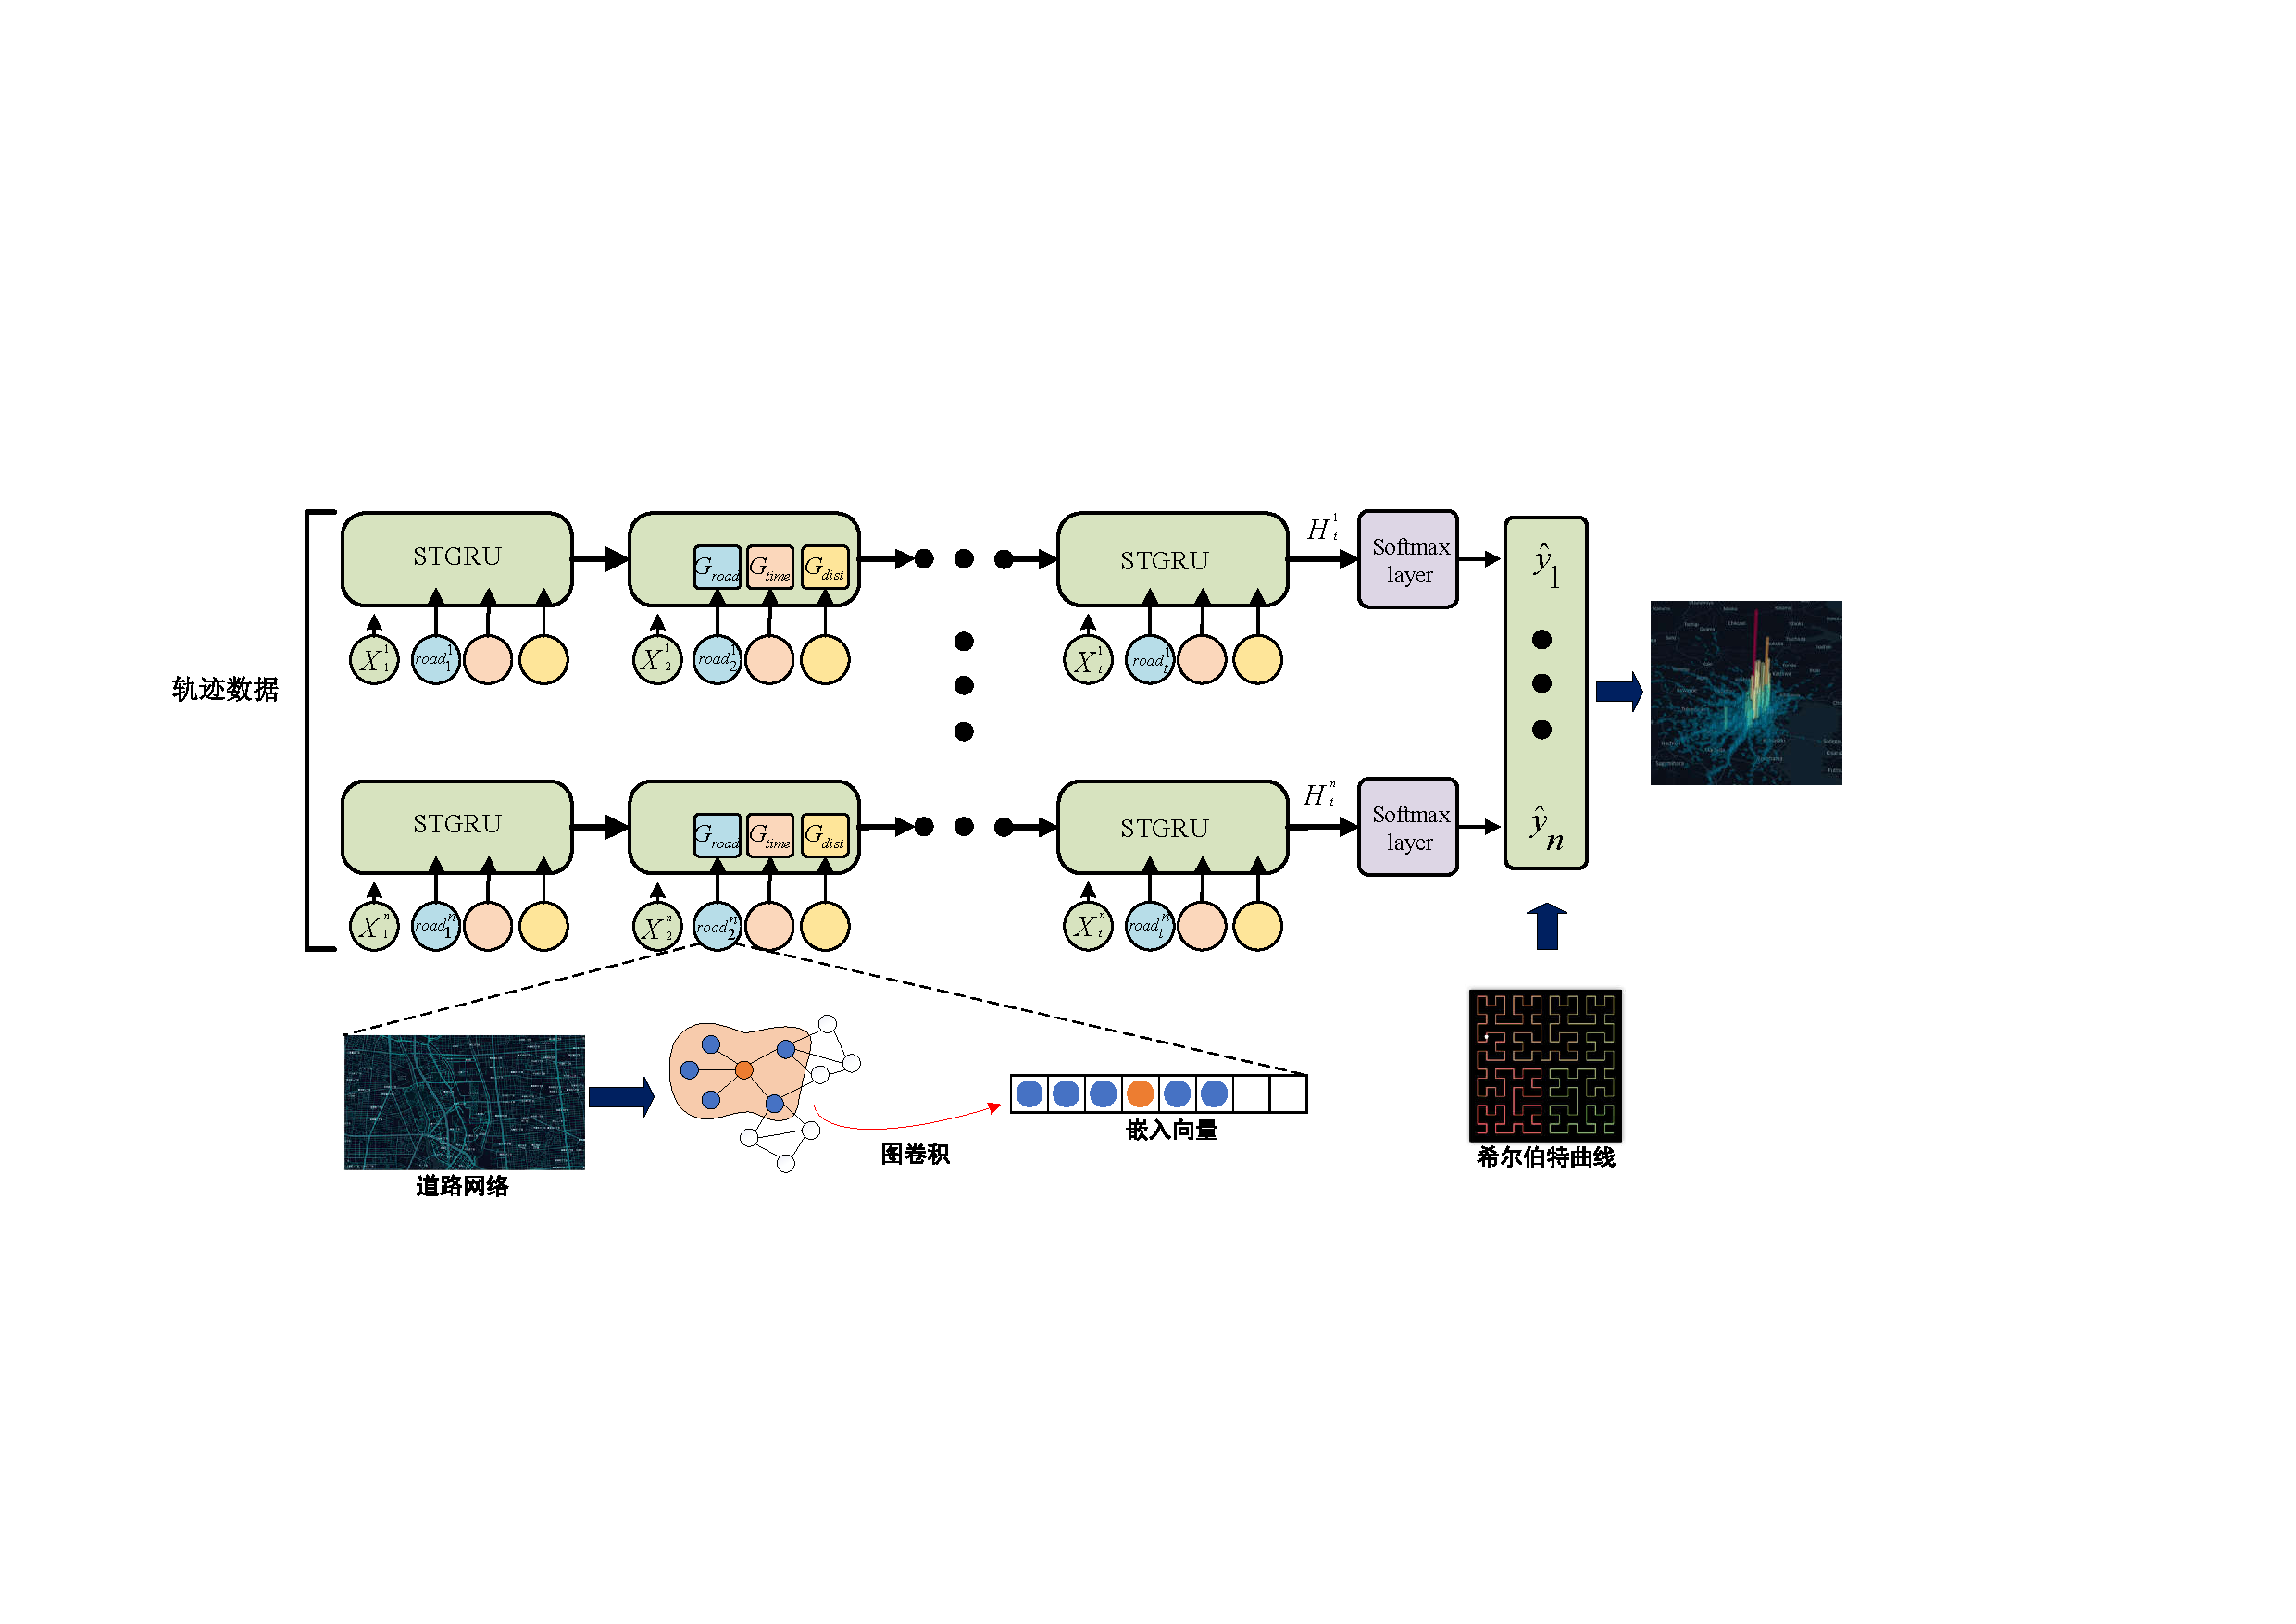
\includegraphics[width=1.0\linewidth]{./pic/stgru_all_3.pdf}
\caption{基于空间特征增强的聚集预测模型}
\label{Figure.4.0.1}
\end{figure*}

如图\ref{Figure.4.0.1}所示为本章提出的基于空间特征增强的聚集预测模型,使用单层STGRU模型对每个用户的位置进行预测,然后对同一时刻所有用户的位置预测结果融合得到得到聚集预测结果。在STRGU模型上堆叠了一个图卷积层提取路网图的节点嵌入向量作为路网门控的输入。其中路网图基于路网结构和用户分布情况构建,路网图的节点嵌入向量包含了路网的空间特征以及用户之间的分布特征。并使用希尔伯特扫描算法生成包含空间特征的区域标签,提升模型的时空特征提取能力。

\subsection{希尔伯特曲线的区域标签生成}
在本节中,首先分析了常用标签生成方法的问题,并介绍了希尔伯特曲线的定义及特性。然后阐述了使用希尔伯特扫描算法生成区域标签的方法。

\subsubsection{常用标签生成方法存在的问题}
\begin{figure*}[!ht]
\centering 
\begin{minipage}[b]{0.45\textwidth}
\centering
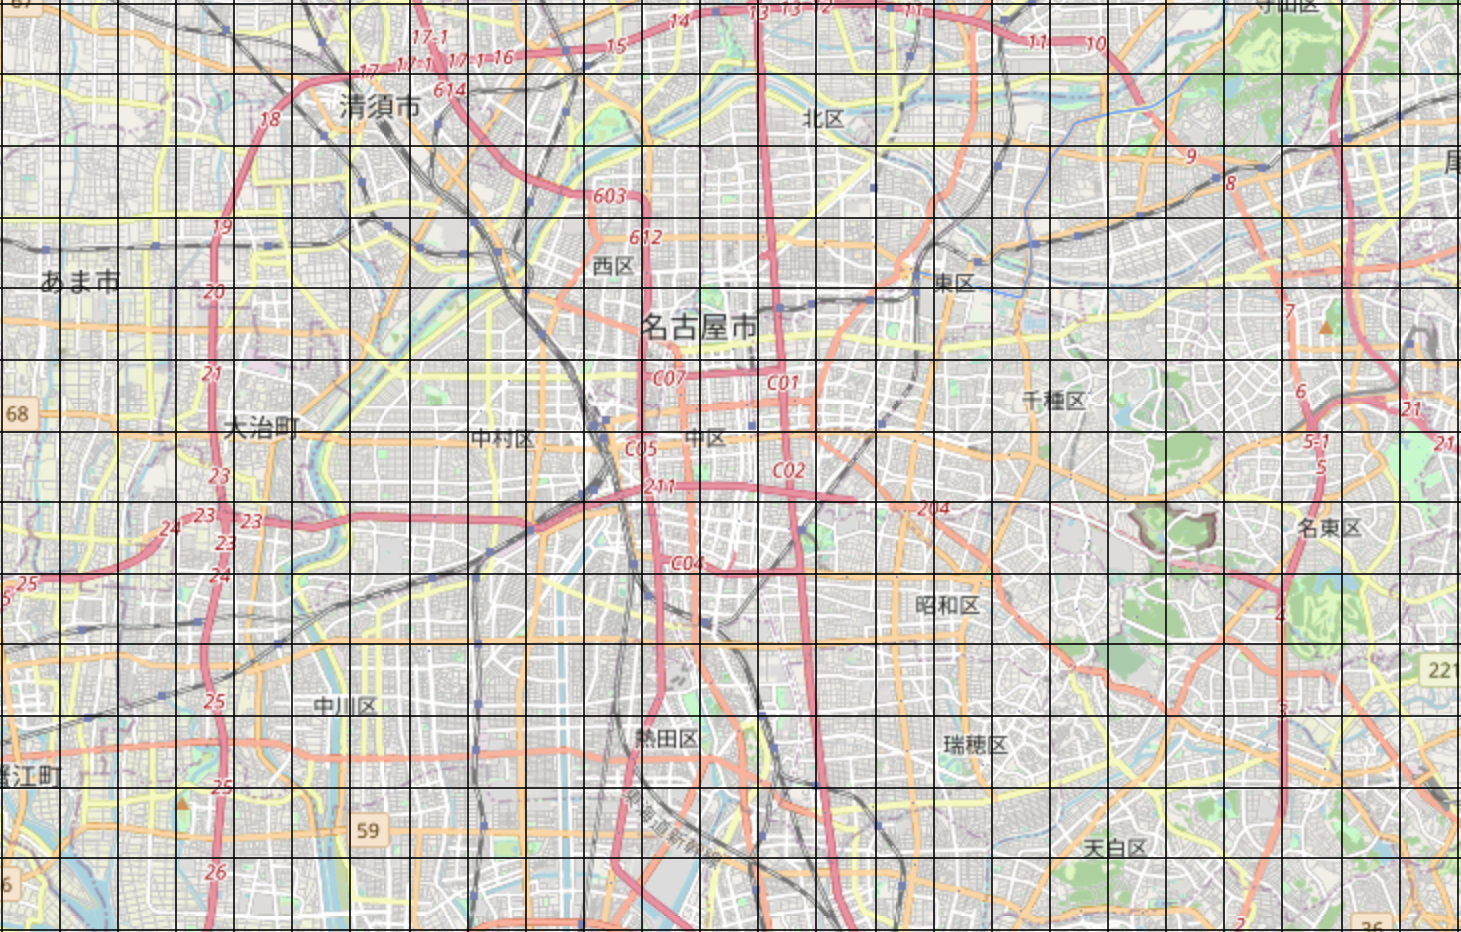
\includegraphics[scale=0.25]{./pic/grid0.png}
\caption{名古屋市部分区域划分情况}
\label{Figure.4.1.1}
\end{minipage}
\begin{minipage}[b]{0.45\textwidth} 
\centering 
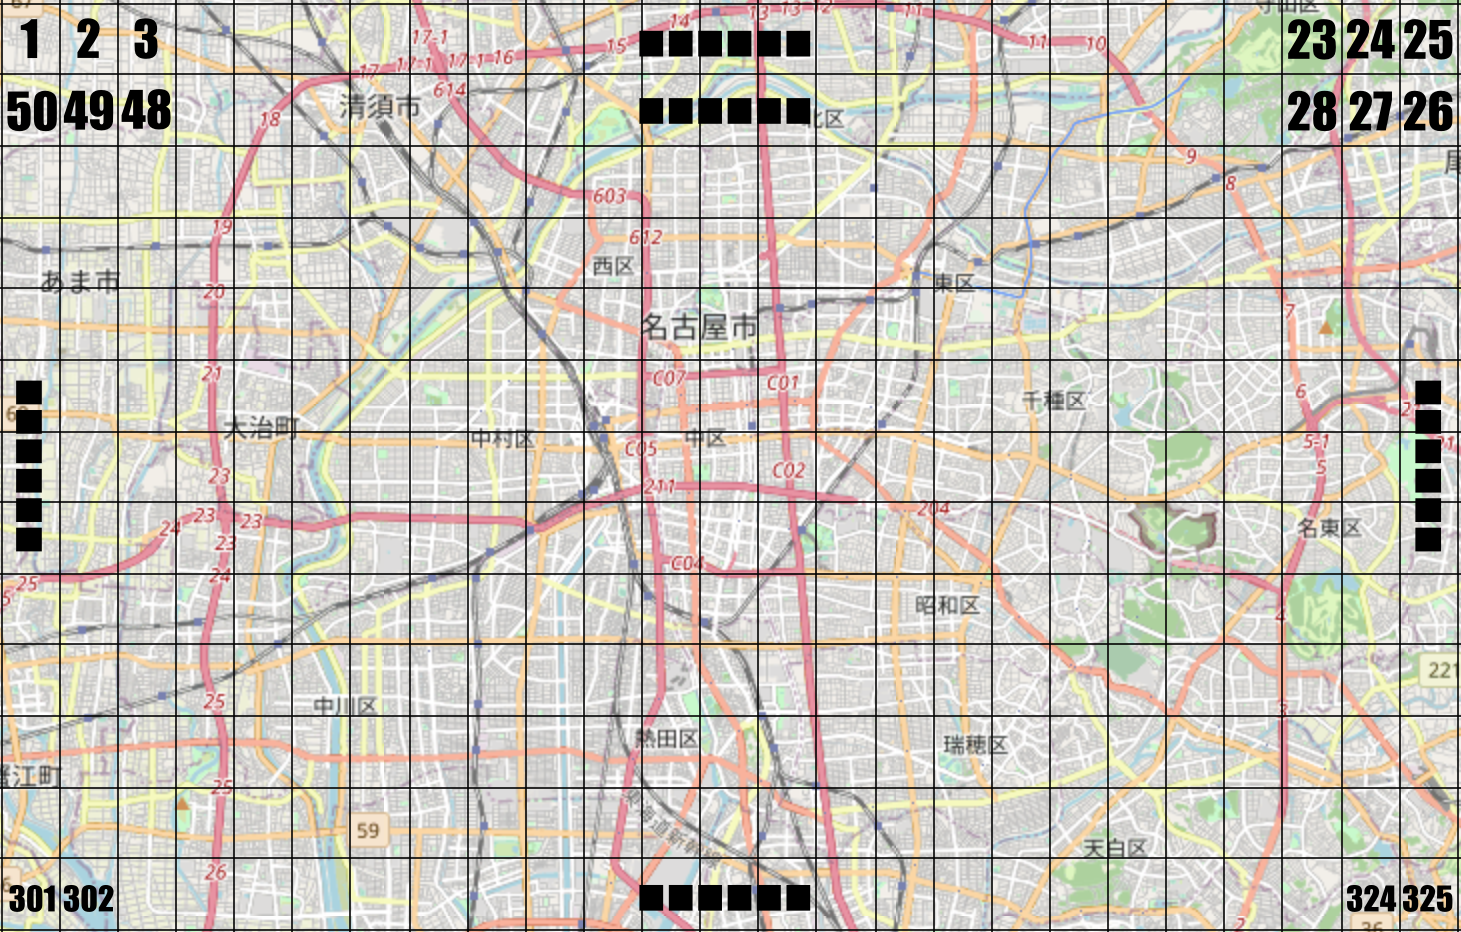
\includegraphics[scale=0.25]{./pic/grid1.png}
\caption{蛇形标签生成示例}
\label{Figure.4.1.2}
\end{minipage}
\end{figure*}
在位置预测任务中,部分工作的目标是预测下一个轨迹点的经纬度,其损失函数为预测值与真实值之间的欧式距离,这类任务属于回归任务。其他工作是预测用户下一个可能出现的地点,如POI推荐,通过计算所有POI的概率进行预测,属于分类任务。本文中将聚集预测转换为基于区域的轨迹预测任务,输出为所有区域的概率值,本质上为多分类任务。POI推荐任务中的标签包含兴趣点的语义特征\citing{DBLP:conf/icwsm/RuizQBF15,DBLP:journals/tkde/YuanZXWZX15},即使经过one-hot或者数值化操作,仍然具有较强的指向型。而区域预测任务中的标签值并不具备语义,因此十分依赖于区域的划分方式以及标签生成的方法。

好的标签生成方法能够大幅减少模型建模难度,提升模型性能。差的标签生成方法会增加数据的复杂性,增加模型建模难度。以最常用的将蛇形编号为例。首先对本文中所使用的名古屋人流数据集\citing{sekimoto2011pflow}所覆盖的区域按前文中使用的参数进行划分,划分后总区域数量为1786个。为了更为清晰的展示,如图\ref{Figure.4.1.1}所示截取了$25\times 13=325$个区域的局部图作为示例,其中每个区域对应一个编号。从左上角开始按蛇形递增,如图\ref{Figure.4.1.2}所示。蛇形编号的方式符合直观的编号逻辑,但是忽视了区域之间的空间关系,隔行相邻的编号之间的空间关系难以表示,且随着划分区域大小的变化编号会随之发生较为复杂的变化。

在讨论区域编号方案的优劣性之前,需要对编号任务进行形式化表示。被编号区域是一个矩形或者正方形区域$R$,需要将其划分为$N$个子区域$\mathcal{R}egions=\{r_1,r_2,\dots,r_N\}$,对每个子区域$r_i$都关联到唯一的编号值。由于编号值具有唯一性,编号$N_{regions} = \{1,2,\dots,N\}$可以视作对区域$R$的压缩,从二维的地理空间压缩成了一维的编号空间。由于编号是一维的,对被编号区域进行编号的过程就相当于一条线迂回穿过每一个子区域,再把线拉伸为得到一条直线,这条直线就是对应的编号空间。

\begin{figure}[!ht]
\centering
\subfloat[]{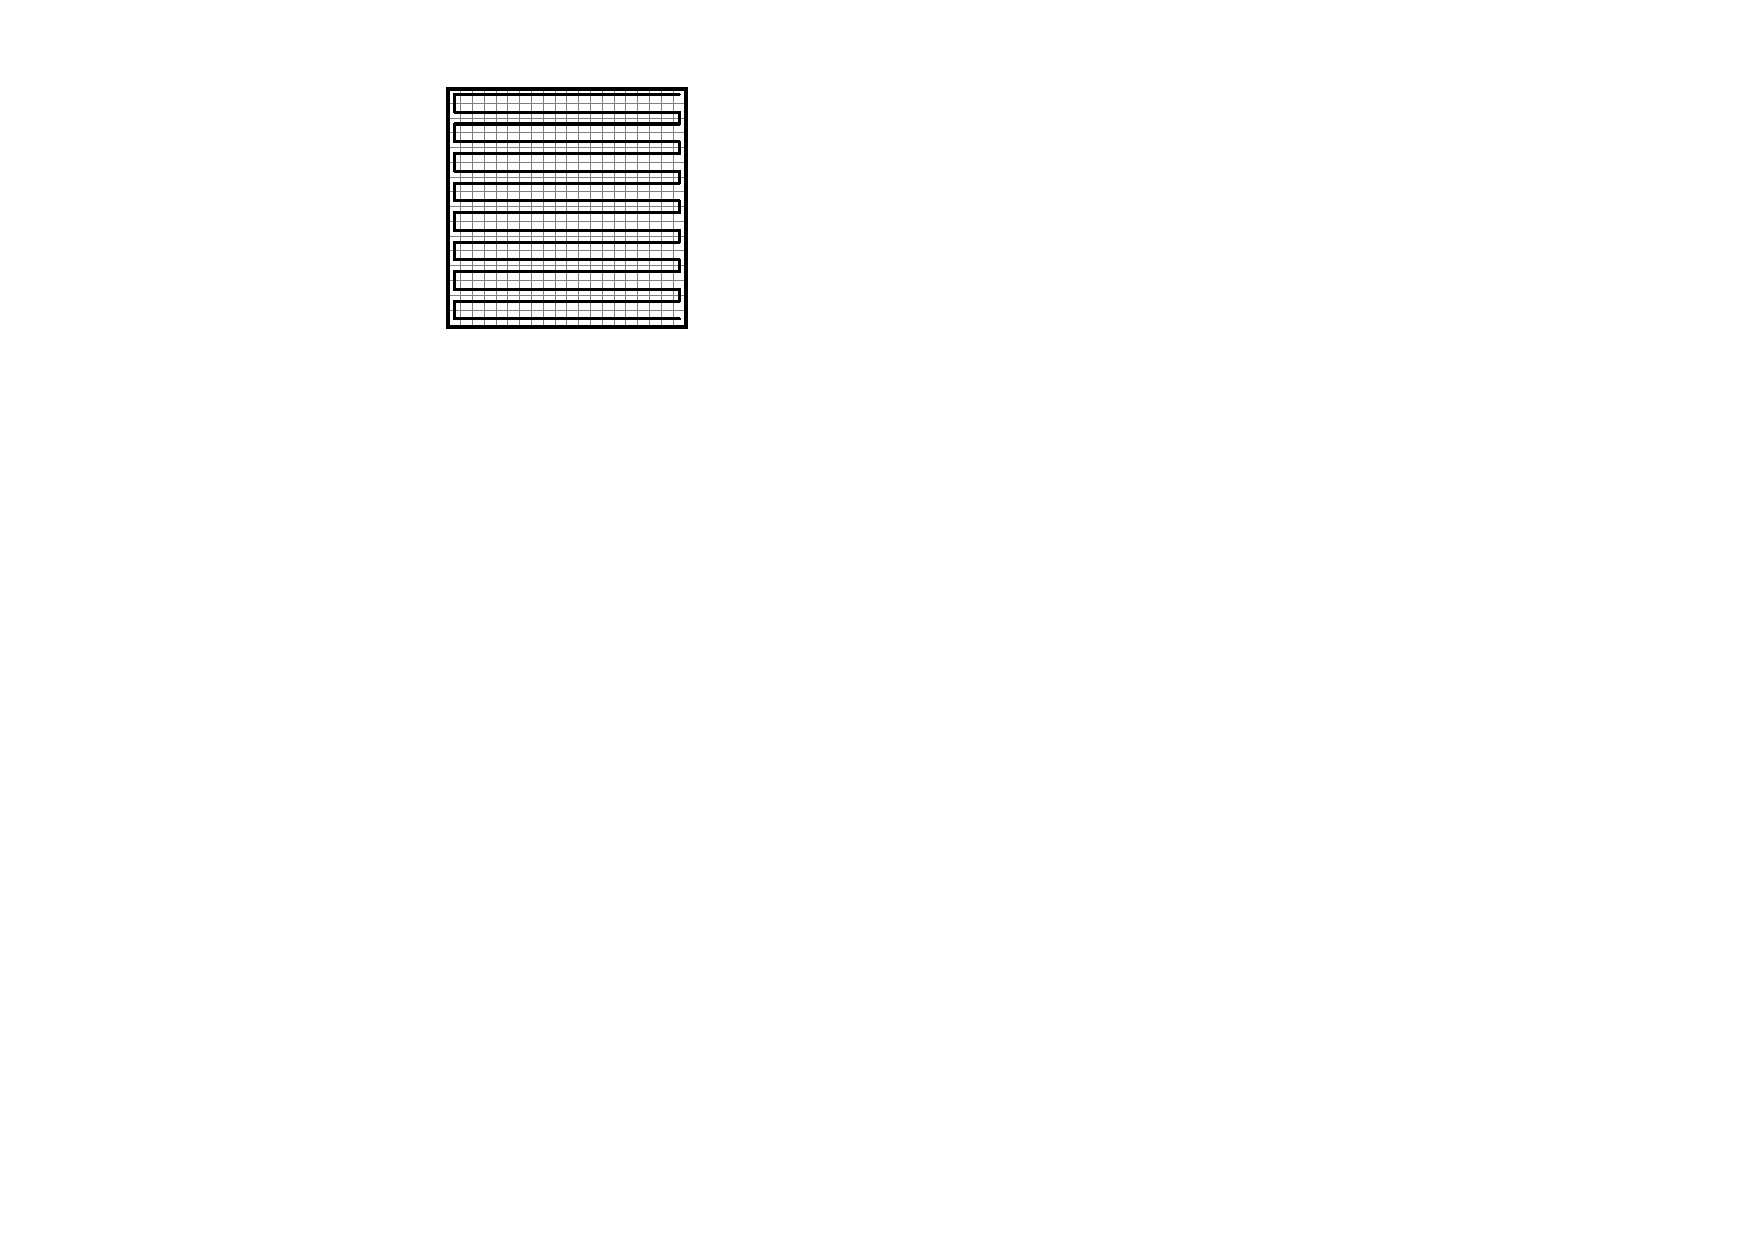
\includegraphics[width=0.32\linewidth]{./pic/snake0.pdf}}
\hfill
\subfloat[]{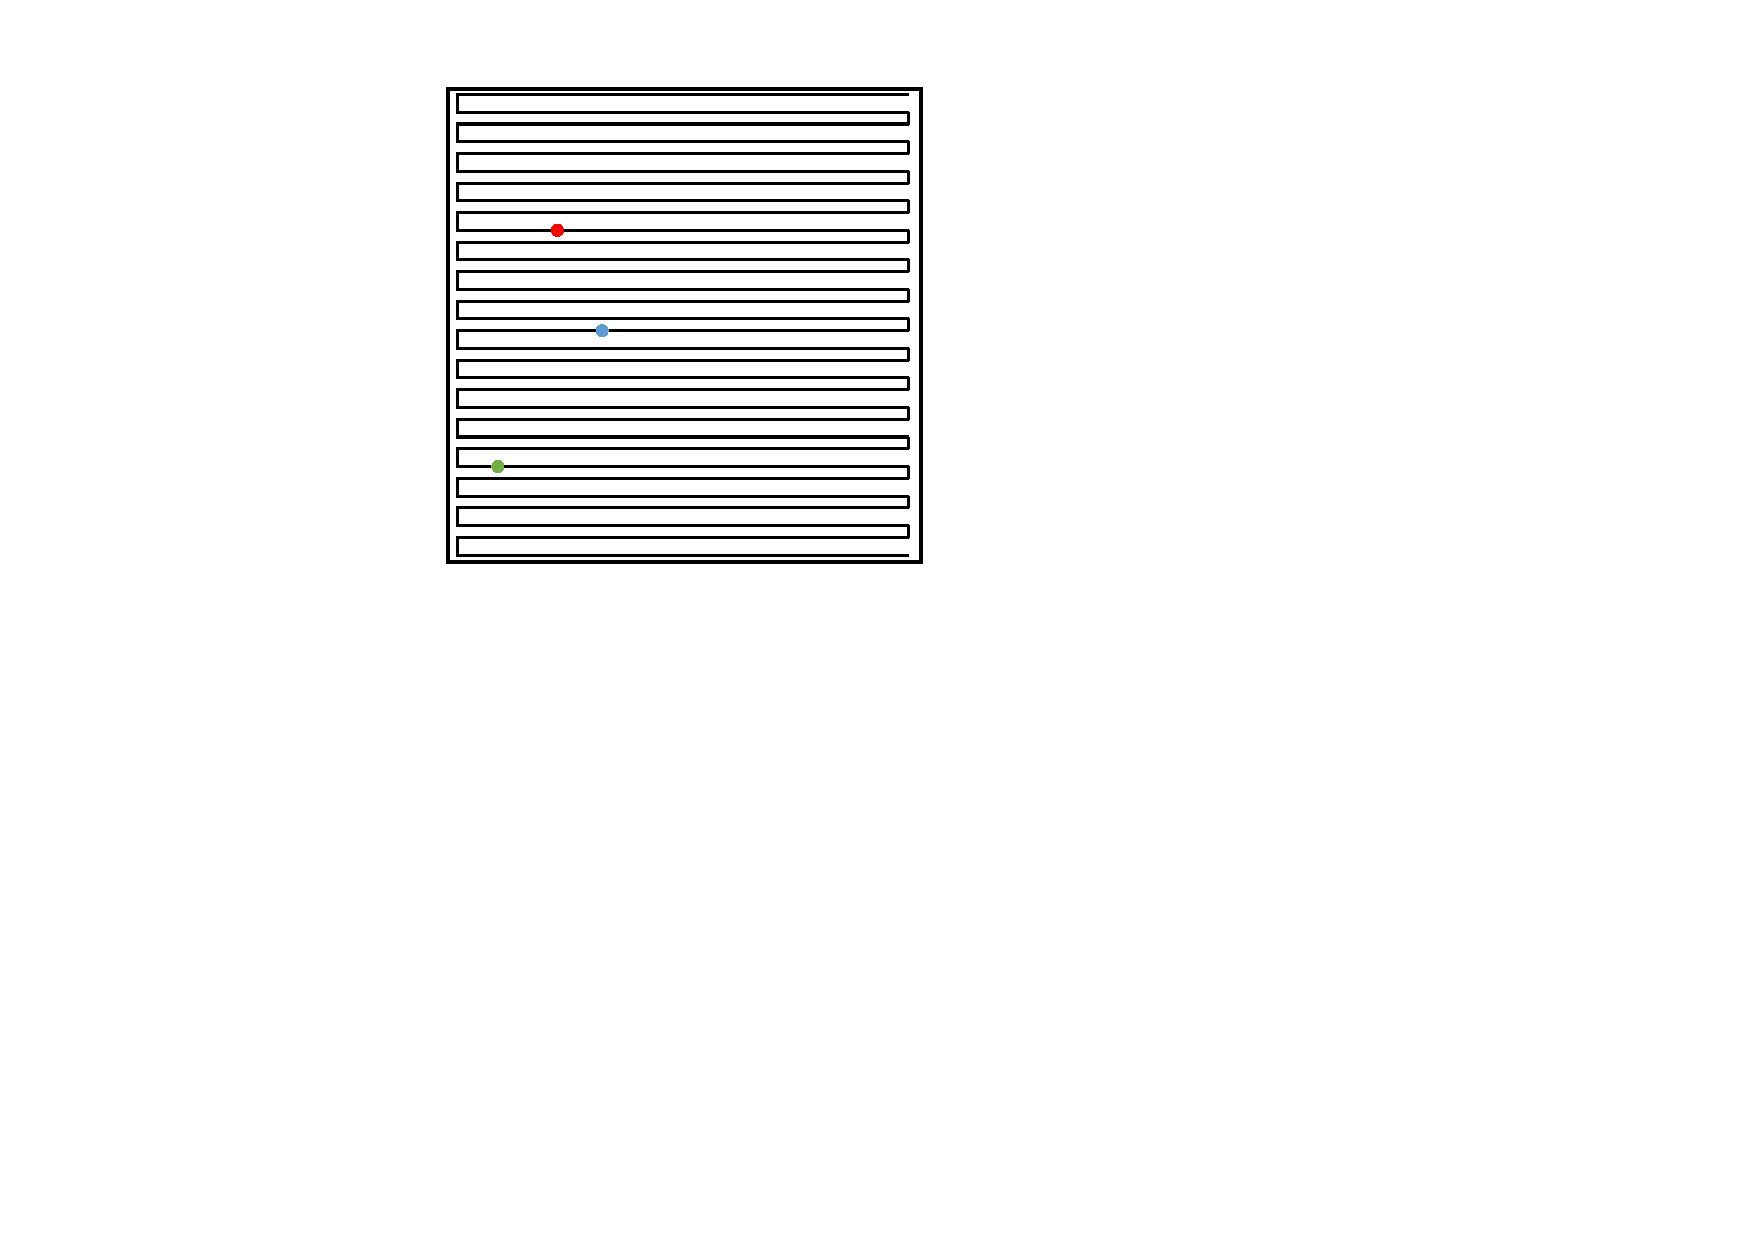
\includegraphics[width=0.32\linewidth]{./pic/snake1.pdf}}
\hfill
\subfloat[]{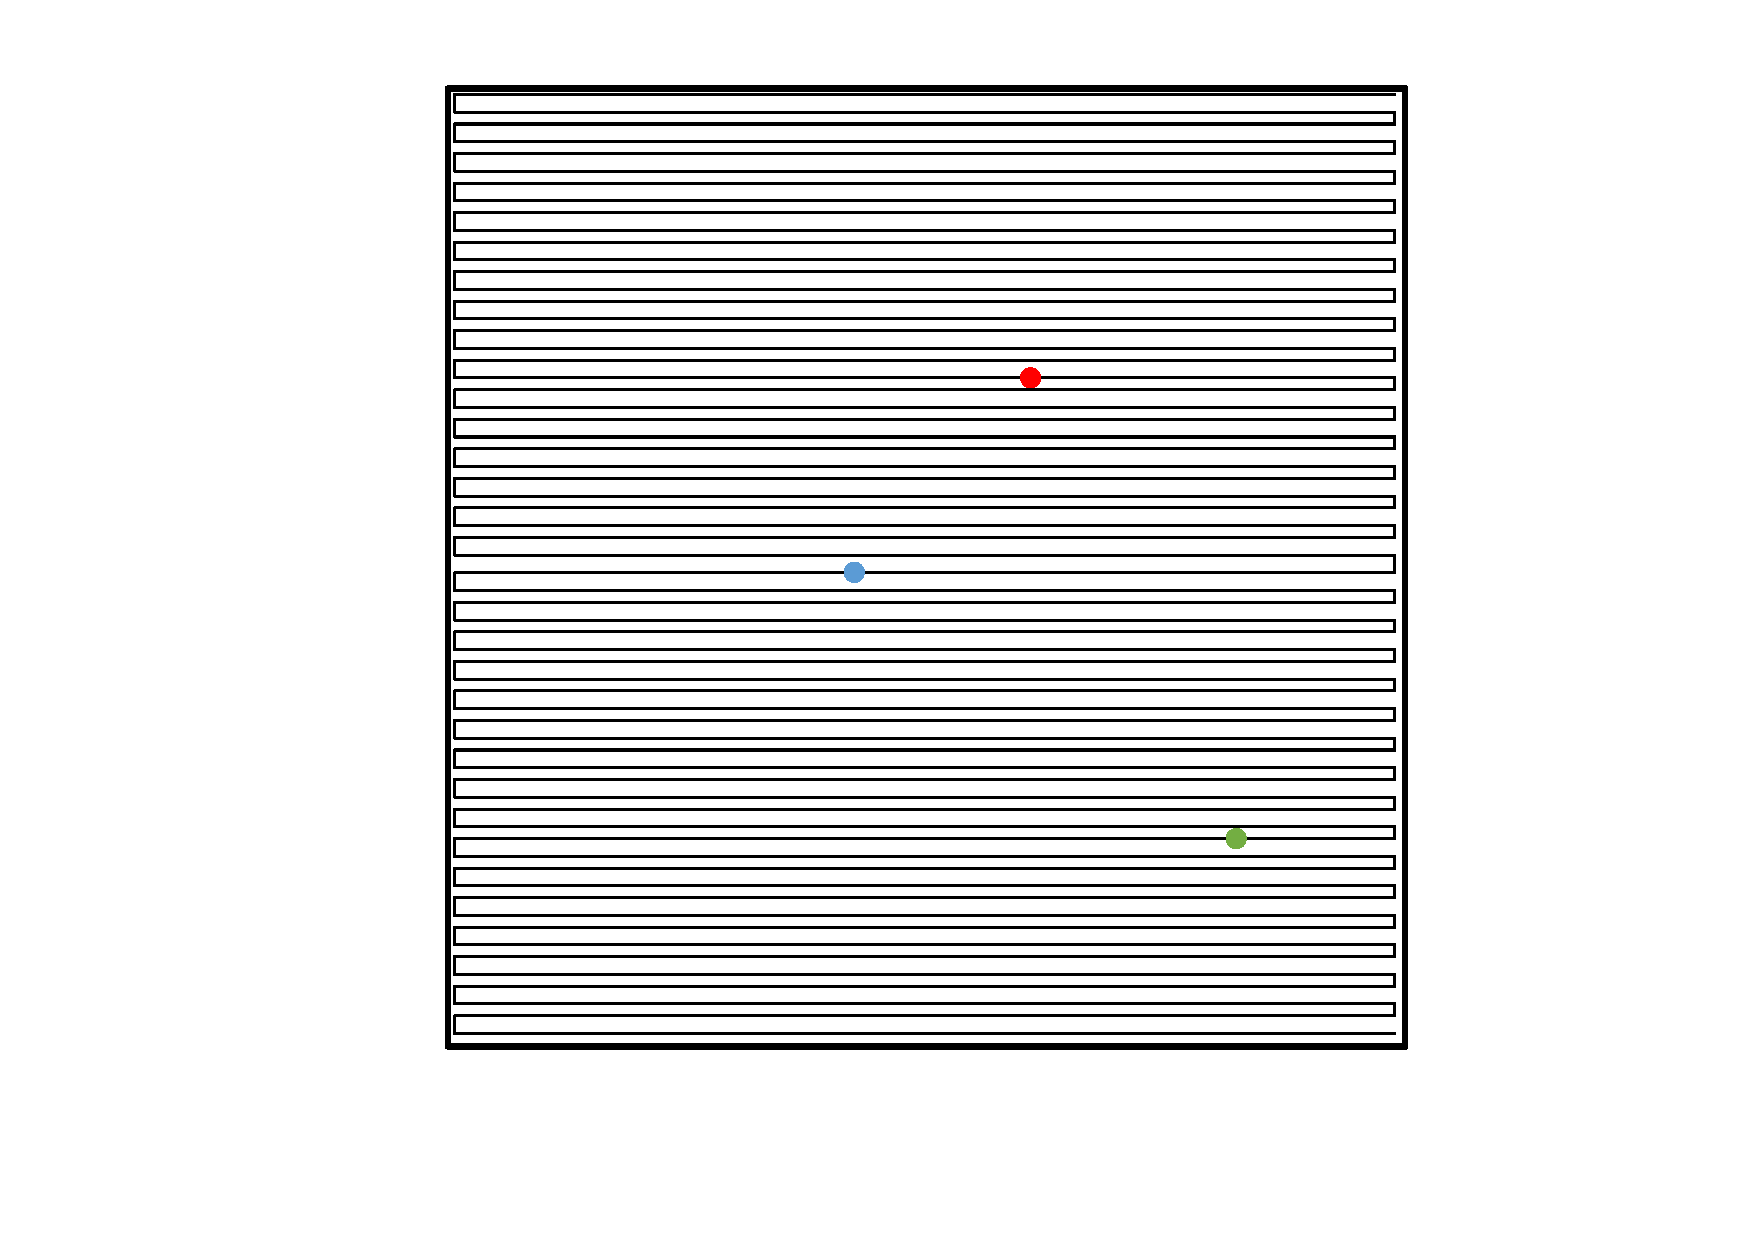
\includegraphics[width=0.32\linewidth]{./pic/snake2.pdf}}
\caption{使用蛇形曲线进行编号。(a)蛇形曲线填充$16 \times 16$比例的正方形区域;(b)蛇形曲线填充$32 \times 32$比例的正方形区域,并标记了三个点;(c)蛇形曲线填充$64 \times 64$比例的正方形区域时被标记点的位置}
\label{Figure.4.1.3}
\end{figure}
最符合直觉的编号方案就是Z字形或者蛇形,此处以蛇形曲线为例,如图\ref{Figure.4.1.3}(a)所示,一次对一行进行编号,在区域空间中交替推进。但是蛇形曲线存在一个严重的问题,当使用不同粒度的子区域进行区域划分时,编号空间中的许多点就会映射到地理空间中完全不同的部分,如图\ref{Figure.4.1.3}(b)和(c)所示,这也就意味着编号与地理空间特征之间的映射较弱。

综上所述,编号方案的好坏取决于根据编号结果对被编号区域空间特征的保留程度,任意两个相邻数值的编号所关联的子区域的距离应该尽可能的小,这样即使对空间特征进行建模的时候存在一定误差,两个值相近的编号也会指向空间中邻近的区域。

\subsubsection{希尔伯特曲线}
\begin{figure*}[!ht]
\centering 
\begin{minipage}[b]{0.45\linewidth}
\centering
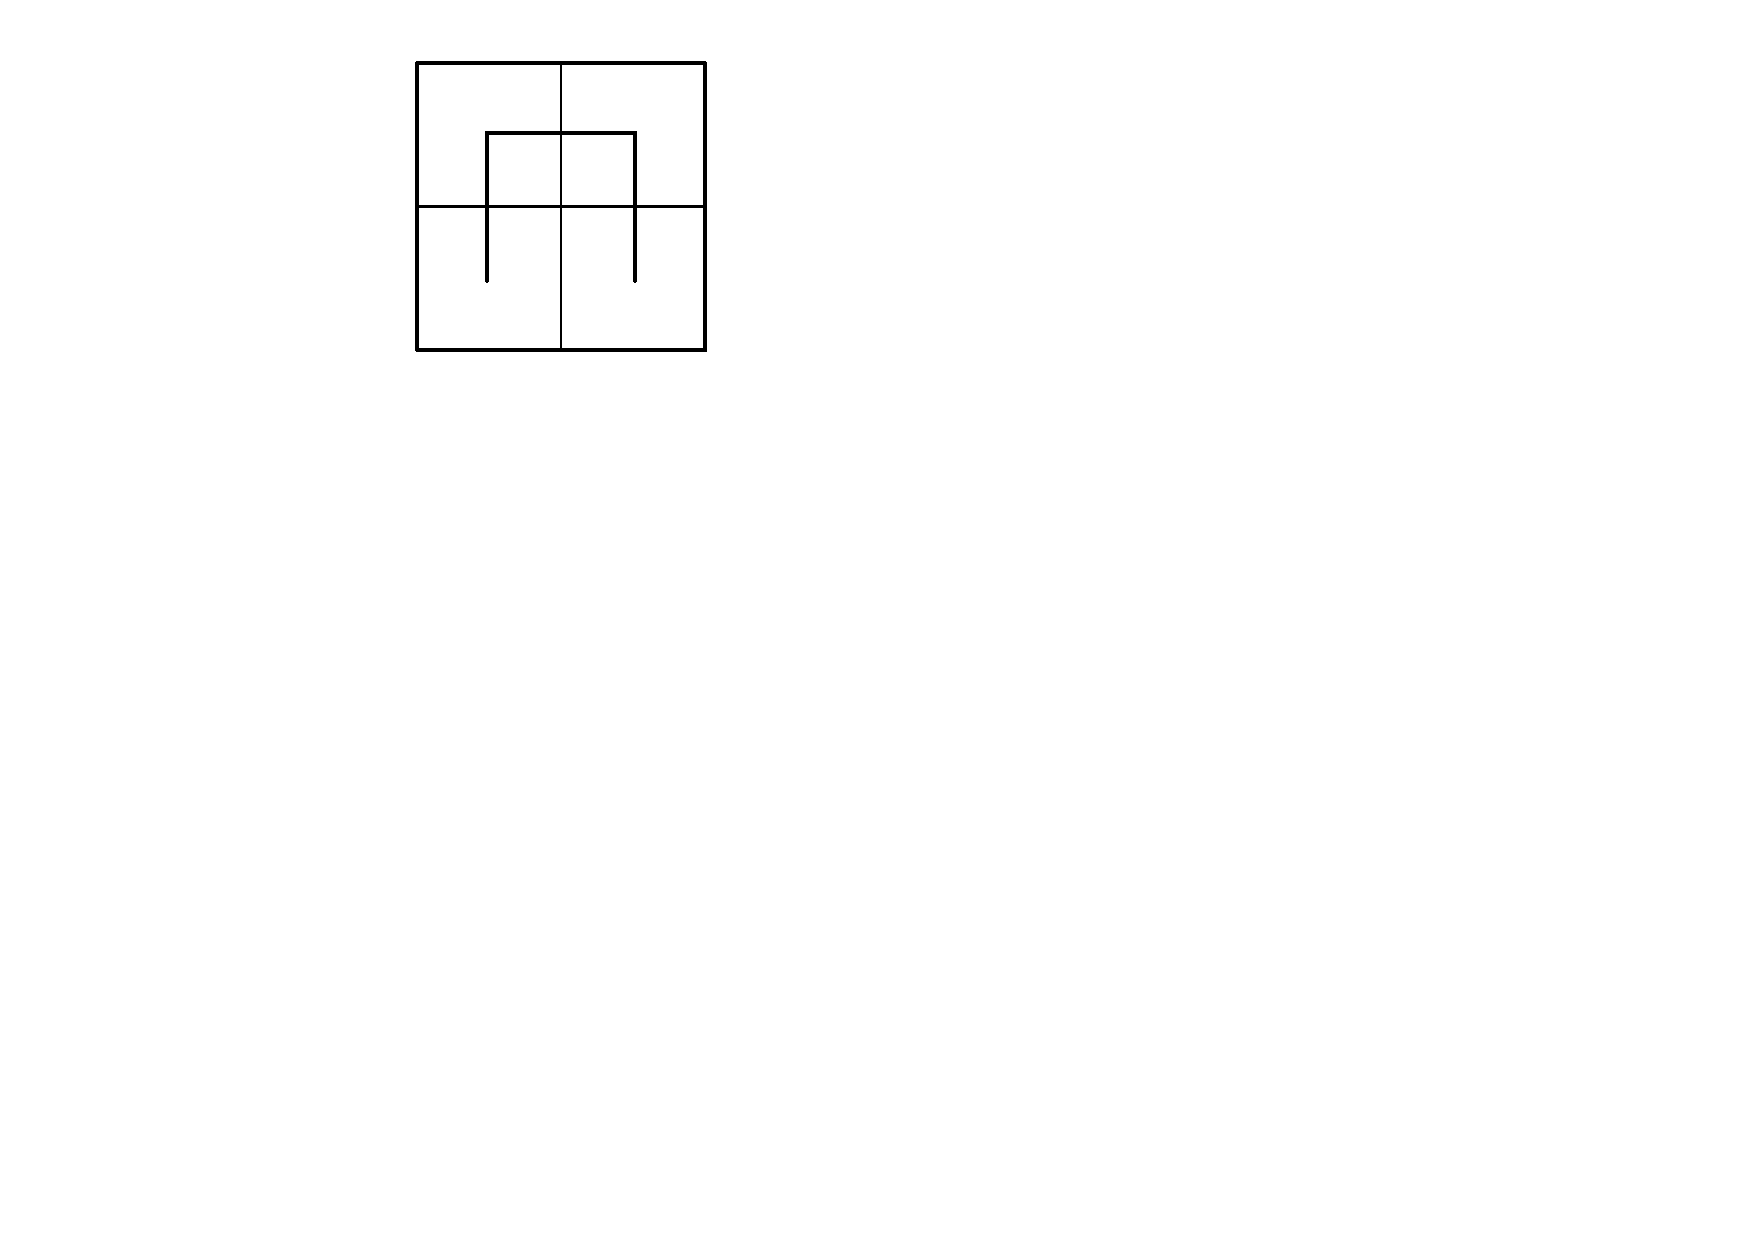
\includegraphics[width=0.7\linewidth]{./pic/hilbert1.pdf}
\caption{1阶希尔伯特曲线}
\label{Figure.4.1.4}
\end{minipage}
\begin{minipage}[b]{0.45\linewidth} 
\centering 
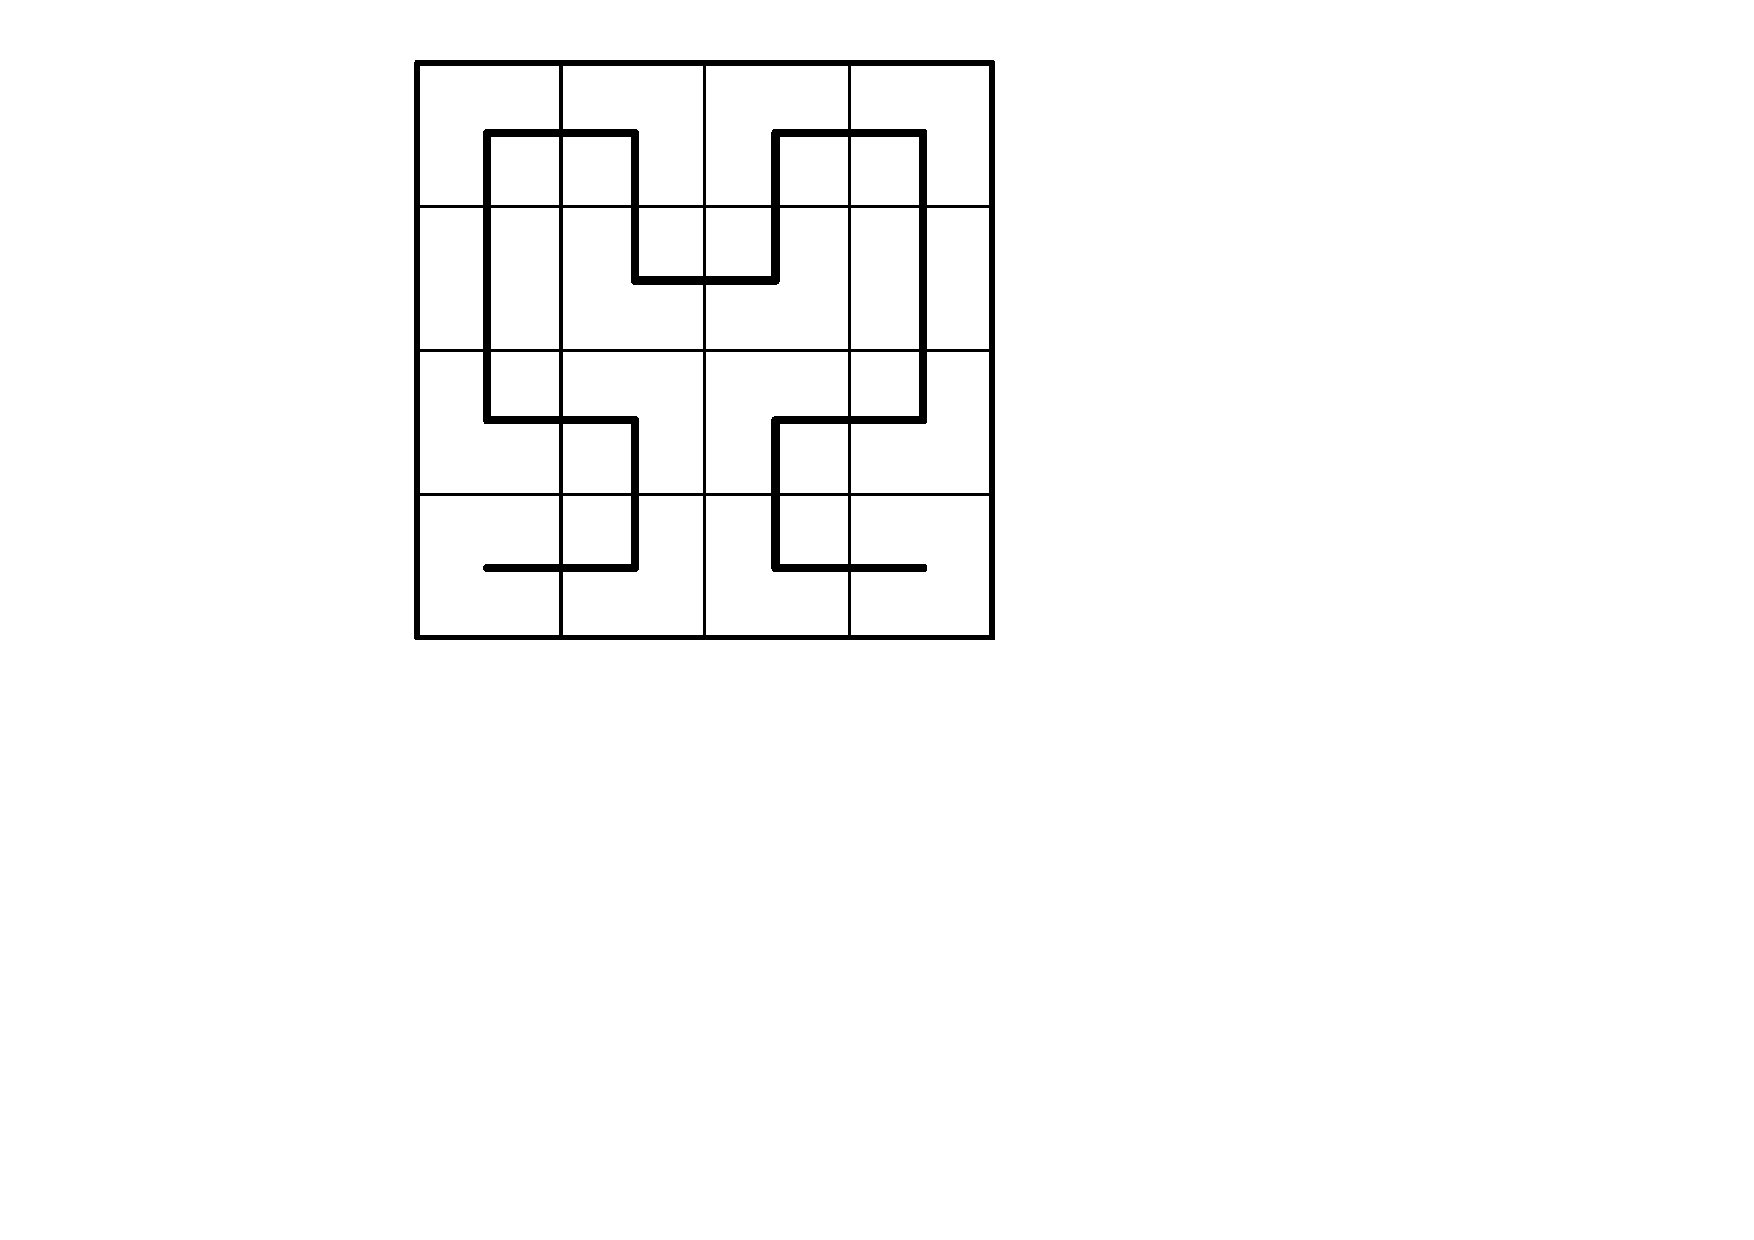
\includegraphics[width=0.7\linewidth]{./pic/hilbert2.pdf}
\caption{2阶希尔伯特曲线}
\label{Figure.4.1.5}
\end{minipage}
\end{figure*}
希尔伯特曲线(Hilbert curves,HC)\citing{hilbert1902mathematical}是一族无限多条的曲线,特定阶数的希尔伯特曲线被称为伪希尔伯特曲线(Pseudo Hilbert curves,PHC),1阶和2阶的希尔伯特曲线如图\ref{Figure.4.1.4}和\ref{Figure.4.1.5}所示。希尔伯特曲线的定义为:

1)希尔伯特曲线是良定义的(well-defined),伪希尔伯特曲线上的点是收敛的,对于所有$x$,对应的$HC_n(x)$是收敛的。
\begin{equation}
\forall t \in [0,1], HC_n(t) = \lim_{n \rightarrow\infty} PHC_n(t)
\end{equation}

2)希尔伯特曲线是连续的。对于值域中的点任意点$(x,y)$,选择一个任意小的$\epsilon$邻域,都可以在其中找到更小的$1/4^k \times 1/4^k$的闭区域,对应到定义域是一个闭区间$I$,可以$I$中在找到更小的$\delta$开区间$I^{\prime}$,$I^{\prime}$中所有点都会映射到值域的$\epsilon$邻域中。

3)希尔伯特曲线能够填充整个空间,即单位正方形中每个点都是希尔伯特曲线的输出。希尔伯特曲线$HC(t)$是从实数$[0,1]$区间到实数平面$[0,1]\times [0,1]$区域上的满射。也就是说给定值域中任意点$(x_i,y_i)$,都能找到对应参数$t_i$使得$HC(t_i)=(x_i,y_i)$。

空间填充曲线的最大优势在于连续性,即输入平稳变化时,输出空间中不会发生跳跃。希尔伯特曲线除连续性之外还具有良定义,即给定一个输入点,随着希尔伯特曲线阶数的上升,对应的输出趋向于空间中的某个点。因此使用希尔伯特曲线进行区域编号能够较大程度的满足相近编号区域在空间中邻近,保留编号之间的空间特征。可以证明希尔伯特曲线可以定义出极限曲线,而前文中的蛇形曲线就无法定义出极限曲线。

\subsubsection{使用希尔伯特扫描算法生成区域编号}
在对数据集中覆盖区域进行编号时发现大多数情况下编号区域是矩形区域。根据希尔伯特曲线能够填充整个空间的特性,只要子区域的大小足够小,理论上是可以使用标准希尔伯特曲线进行填充,但不能满足所有使用场景。在数字图像处理领域,Kamata等人\citing{DBLP:conf/icip/KamataB97,DBLP:journals/tip/KamataEB99}和Zhang等人\citing{DBLP:conf/iwicpas/ZhangKU06}先后提出了多种希尔伯特扫描算法,首先使用将矩形块划分为块的分割方法,然后基于查找表的方法提出每个块中地址的配置方法。

在对矩形区域进行编号时,需要先生成自定义大小的矩形区域的希尔伯特曲线填充数组,再根据经纬度及划分粒度计算出待编号区域的下标,并根据希尔伯特曲线填充数组中的对应值进行编号。本章实现了二维希尔伯特扫描算法generate2d,伪代码如算法\ref{alg:algorithm1}所示,其中$\mathrm{sgn}$函数为符号函数:
\begin{equation}
\mathrm{sgn}(x)=
\begin{cases}
1,\quad &x>0\\
0,\quad &x=0\\
-1,\quad &x<0
\end{cases}
\end{equation}

\begin{algorithm}[!ht]
\SetAlgoLined
\KwData{$(x,y,ax,ay,bx,by)$\\第一次调用时的参数为:$x=0,y=0,ax=width,ay=0,bx=0,by=heigth$\\}
\KwResult{编号后的二维数组$\mathcal{A}$}
\Begin{
    $w = |ax+ay|,h = |bx+by|$\\
    计算希尔伯特曲线填充时的主方向$(dax, day) = (\mathrm{sgn}(ax),\mathrm{sgn}(ay))$\\
    正交方向为$(dax, day) = (\mathrm{sgn}(bx),\mathrm{sgn}(by))$\\
    \uIf{$h == 1$}{
        \ForEach{$i \in [0,w)$}{
            $\mathbf{yield}\quad (x,y) = (x+dax\times i, y+day\times i)$\\
            \Return
        }
    }
    \uIf{$w == 1$}{
        \ForEach{$i \in [0,h)$}{
            $\mathbf{yield}\quad (x,y) = (x+dbx\times i, y+dby\times i)$\\
            \Return
        }
    }
    $(ax_2,ay_2) = (ax//2, ay//2),(bx_2,by_2) = (bx//2, by//2)$\\
    $w_2 = |ax_2+ay_2|,h_2 = |bx_2+by_2|$\\
    \eIf{$2w>3h$}{
        分为两个部分进行递归填充\\
        $\mathbf{yield}\quad generate2d(x,y,ax_2,ay_2,bx,by)$\\
        $\mathbf{yield}\quad generate2d(x+ax_2,y+ay_2,ax-ax_2,ay-ay_2,bx,by)$
    }{
        标准情况:分为上、下、水平三部分\\
        $\mathbf{yield}\quad generate2d(x,y,bx_2,by_2,ax_2,ay_2)$\\
        $\mathbf{yield}\quad generate2d(x+bx_2,y+by_2,ax,ay,bx-bx_2,by-by_2)$\\
        $\mathbf{yield}\quad generate2d(x+(ax-dax)+(bx_2-dbx),y+(ay-day)+(by_2-dby),-bx_2,-by_2,-(ax-ax_2),-(ay-ay_2))$
    }
}
\caption{二维希尔伯特扫描算法generate2d}
\label{alg:algorithm1}
\end{algorithm}

\subsection{路网图构建及轨迹点匹配}
路网结构信息与用户的分布状态存在十分直观的联系\citing{DBLP:conf/kdd/Wang0SCJSC20},为了能够更充分利用路网结构信息以及建模用户之间的关联性,需要充分考虑道路之间的拓扑结构\citing{DBLP:journals/cor/BoyaciDL21}。路网拓扑结构通过路网图表示,构建路网图\citing{DBLP:conf/iconip/OwakiM20}最直观的方式就是将道路交叉点视为节点,道路视为图的边,这样的构建方式更侧重于交通情况的建模,不符合本章构建路网图的出发点。受Jiang等人\citing{DBLP:journals/ijgi/LinB17}的启发,利用图对偶的方式,用节点表示道路,道路之间的连通性为边构建路网图。

\begin{figure*}[!ht]
\centering 
\begin{minipage}[b]{0.45\textwidth}
\centering
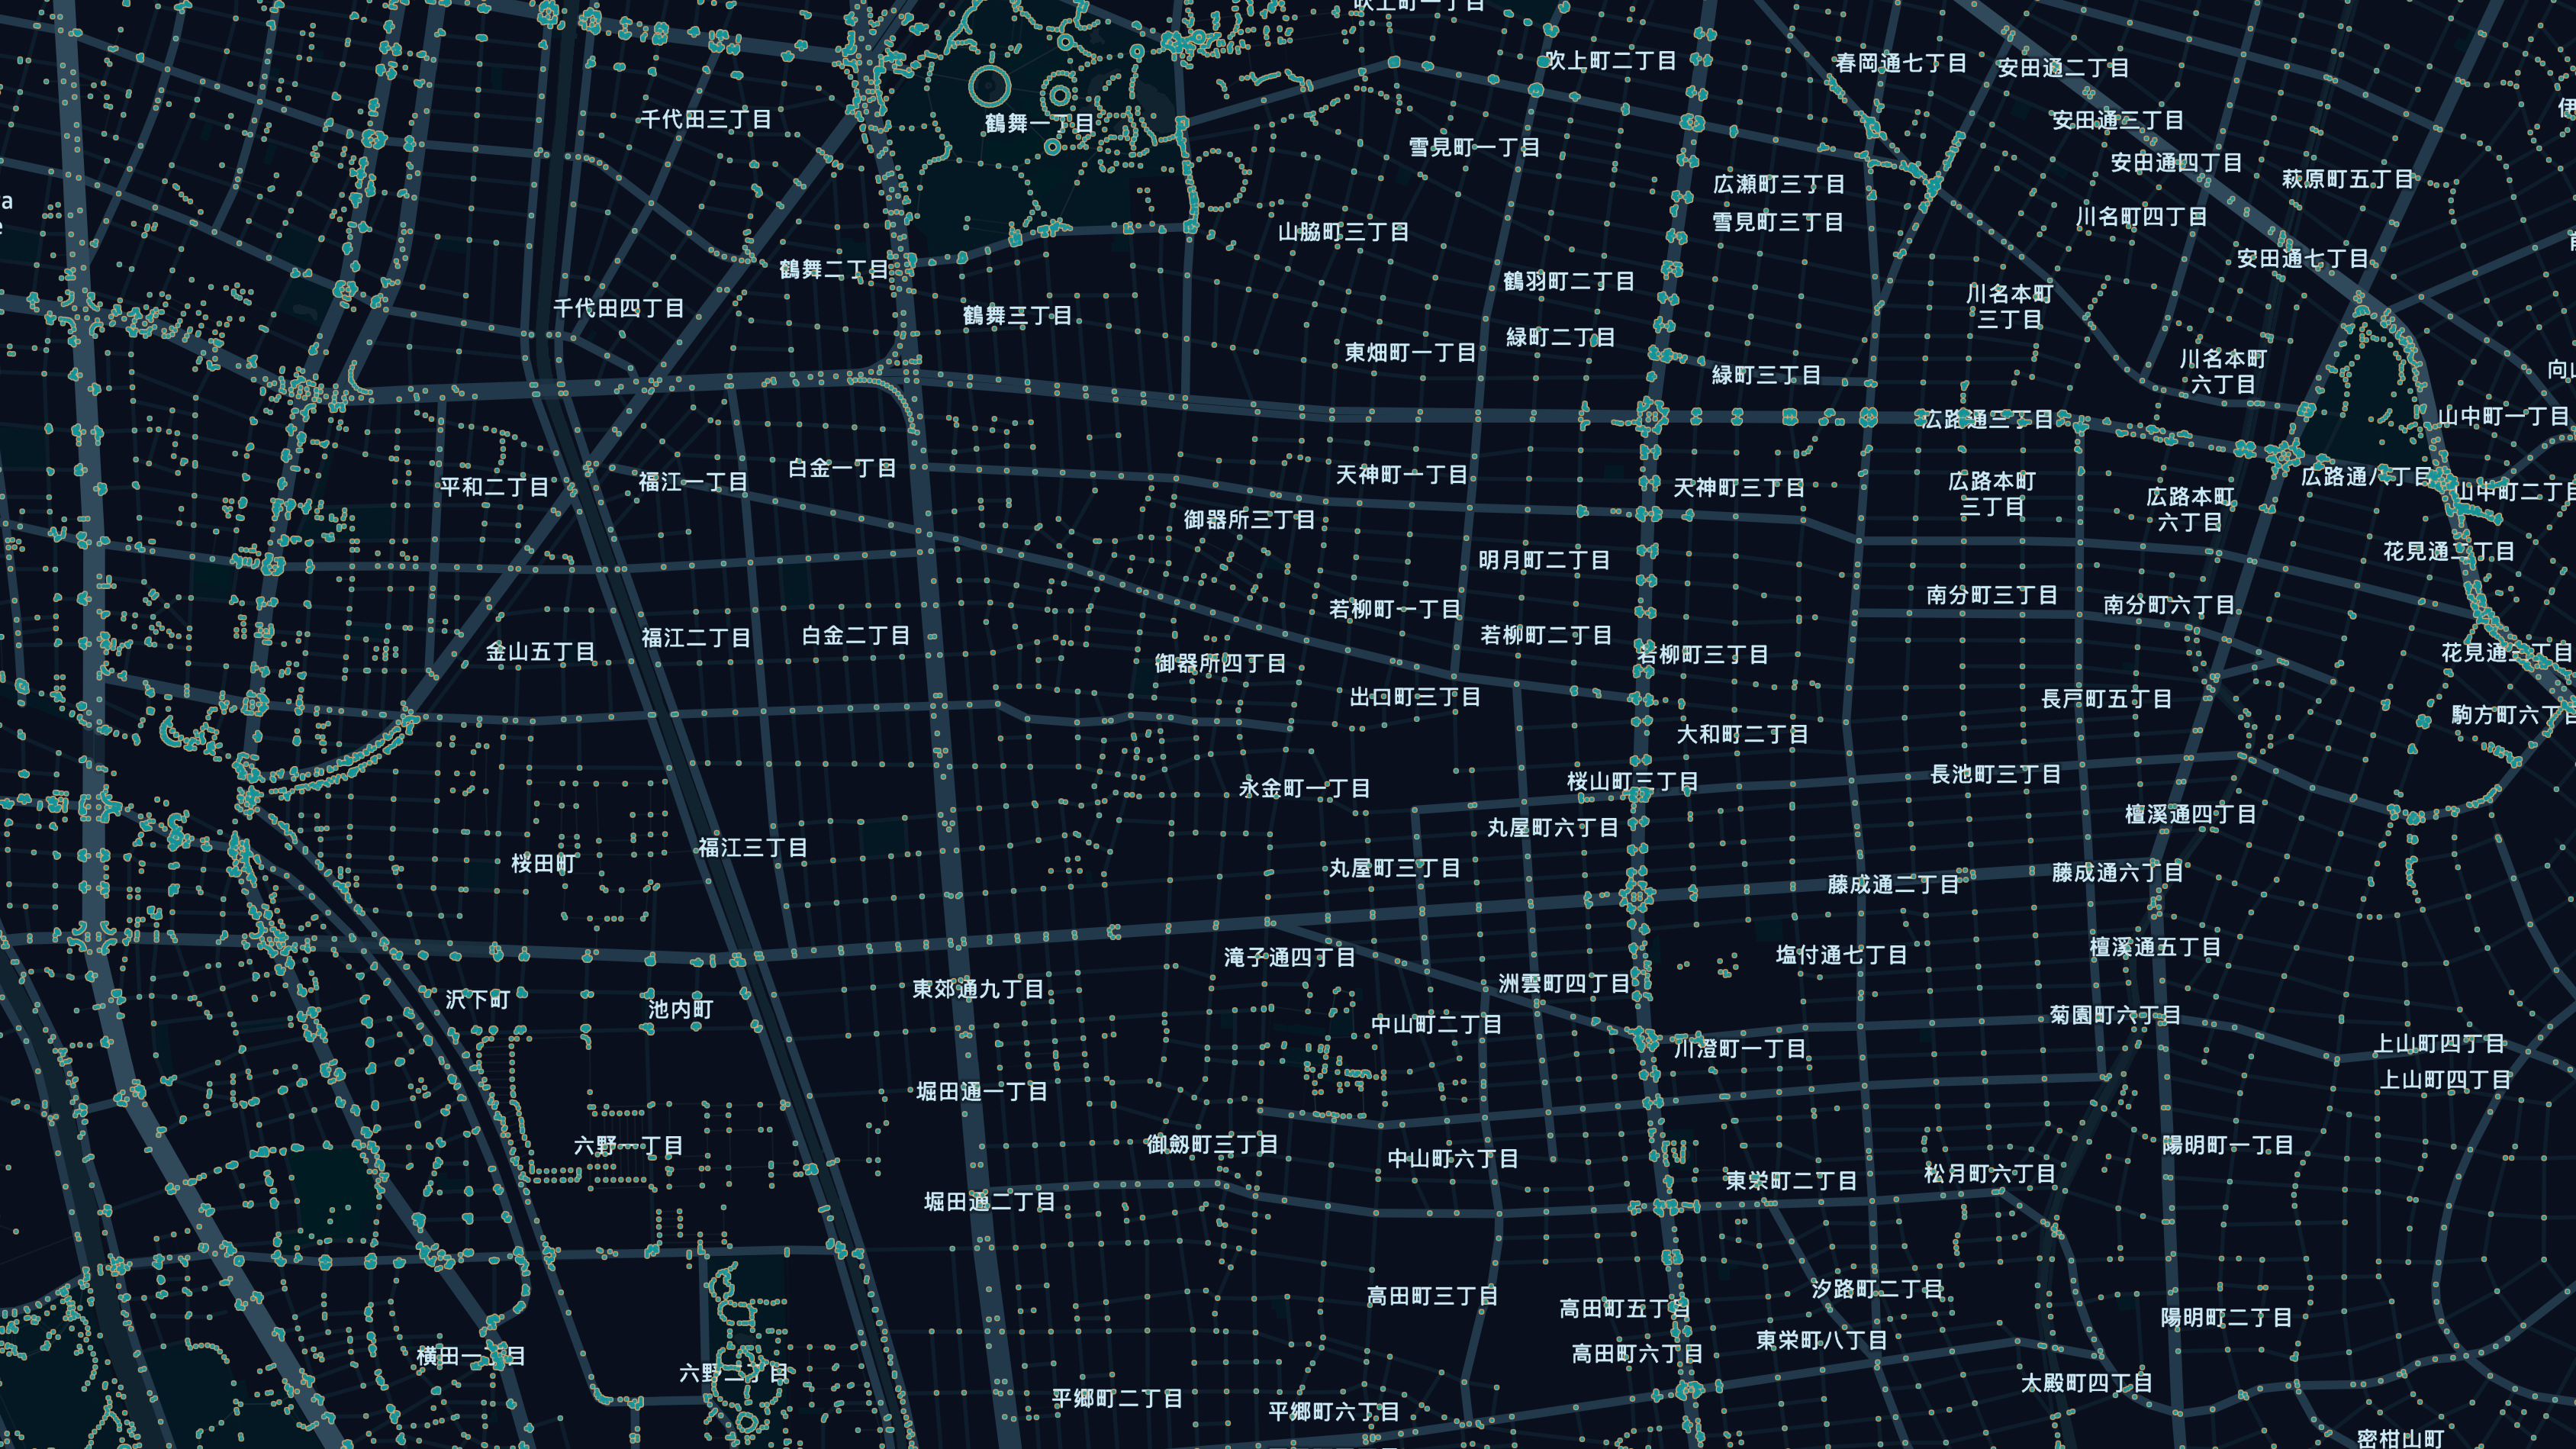
\includegraphics[scale=0.1]{./pic/node1.png}
\caption{部分道路节点图}
\label{Figure.4.2.1}
\end{minipage}
\begin{minipage}[b]{0.45\textwidth} 
\centering 
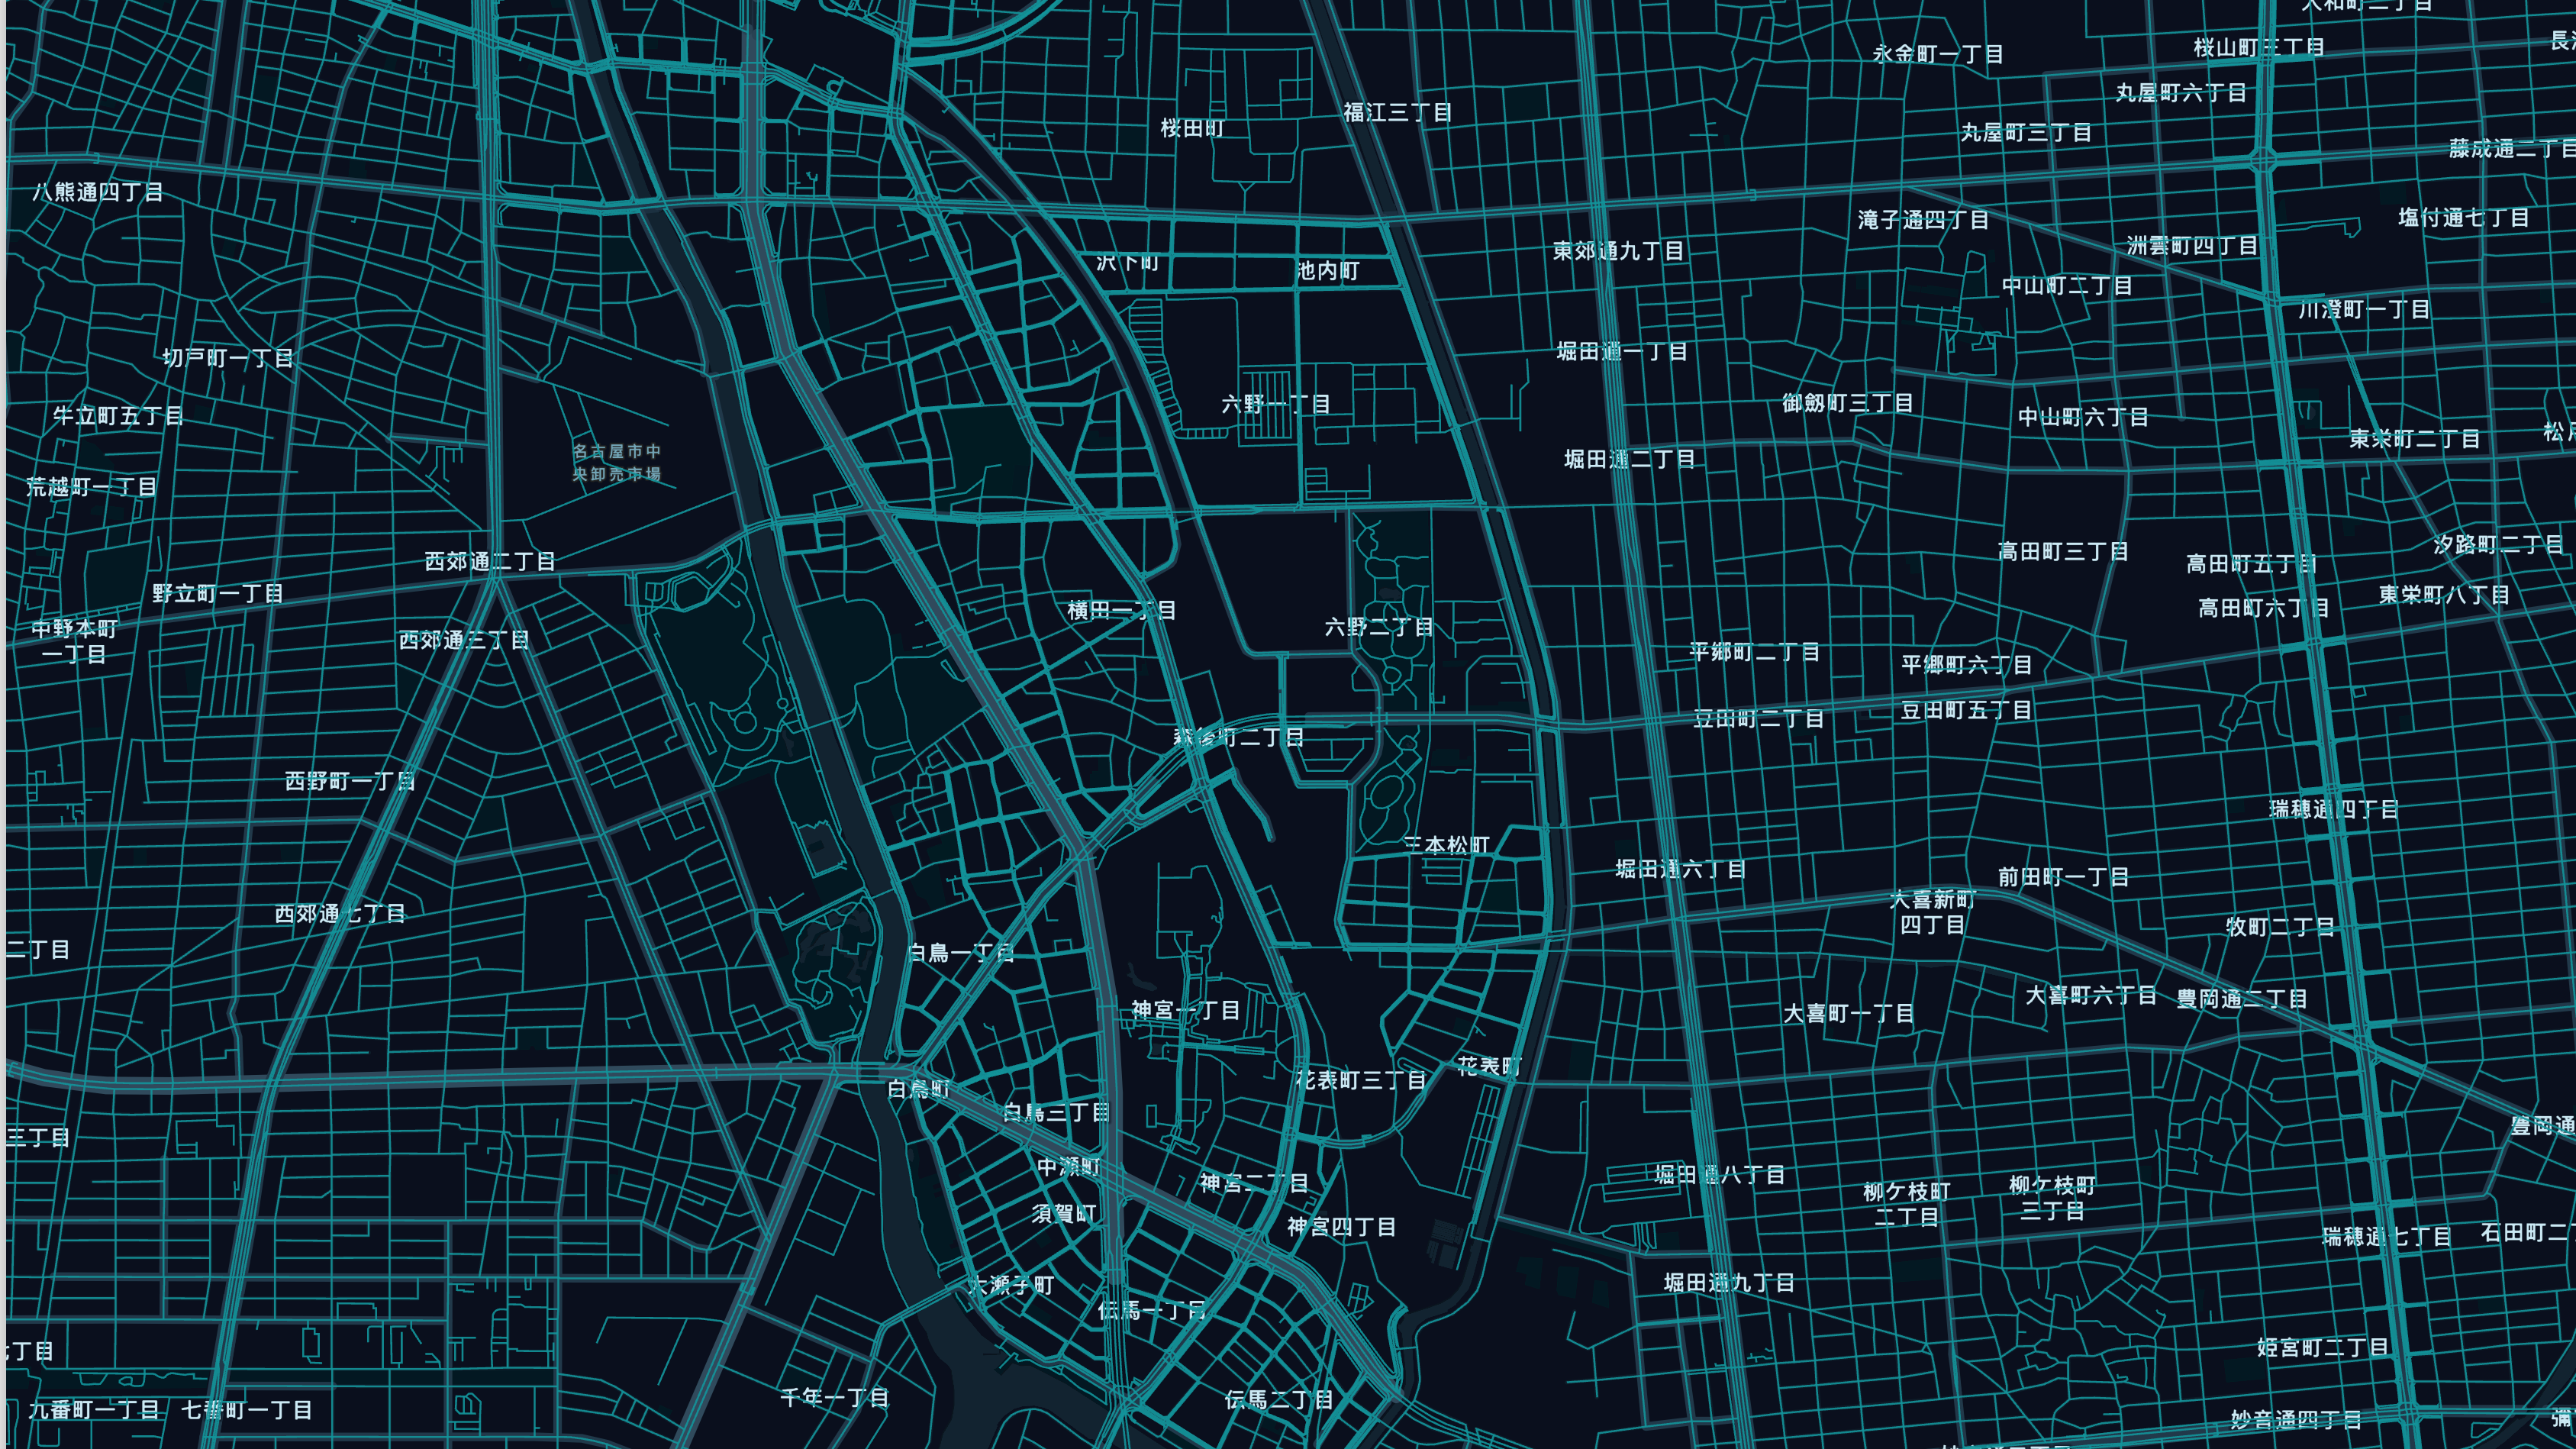
\includegraphics[scale=0.1]{./pic/road1.png}
\caption{部分路网图}
\label{Figure.4.2.2}
\end{minipage}
\end{figure*}

如图\ref{Figure.4.2.1}和图\ref{Figure.4.2.2}所示,分别为名古屋市道路网络中部分节点信息和道路网络的可视化,在地理信息领域\citing{DBLP:journals/lgrs/YangZW22}通常采用GeoJson进行表示,在GeoJson中的道路由string类型组成,称之为路段。每个路段通常为一条直线,由多个离散的节点按顺序连接得到,路段之间的连接关系则表示为头尾节点的连接。因此,可以通过判断两个路段是否存在重叠节点判断连接与否。在地理信息领域中的道路有国道、省道、县道等级别,长度也是在数十公里到数百上千公里不等。如果将一条道路视为一个节点,那么得到的路网图会是一个节点较少且节点度较大的稠密图,这很难对用户在城市场景下的局部路网结构进行表示。

本章采用路段为节点,路段之间的连通关系为边的方式构建路网图,即两个有公共节点的路段之间视为存在边,主要原因为基于路段的路网图能够更好的与用户分布轨迹点进行匹配。基于路段的路网图节点数量较多,以名古屋市为例,节点数约为1,500,000个,东京市路网中的路段数甚至达到了2,500,000个,且每个节点边数较为稀少,能够更精确的表示用户的分布信息和更方便建模局部区域的路网结构。于是路网图可以定义为$\mathcal{G}=(\mathcal{E},\mathcal{V},\mathcal{A})$,其中$\mathcal{V}=\{v_0,v_1,\dots,v_n\}$是由$n$个节点构成的集合,包含了路段的ID、名称、类别等信息,$\mathcal{E}$是图中所有边的集合,$\mathcal{A}$是一个$1\times n$的向量,表示每个节点上存在的用户数量。

由于采集设备的精度问题以及当前路网的表示原因,数据集中的大部分轨迹点与路网节点之间是存在一定偏差的,因此需要将轨迹点与路网图中的路段节点进行一一对应,先计算轨迹点与路网节点之间的距离,再取距离最近轨迹点与路网节点进行匹配。由于路网图节点数量众多,暴力匹配算法的时间复杂度将会成倍增加,以名古屋市的人流数据集为例,轨迹点数约为1,000,000个,路网图节点数约为1,500,000个,暴力匹配算法需要计算约$1.5\times 10^{12}$次节点距离,每次计算两个节点之间的距离需要两次减法、两次乘法运算、一次加法运算以及一次开方运算,并需要对每个轨迹点与所有节点的距离进行排序,以快速排序为例,也需要$O(n\log n)$约为$1.5\times 10^9$次比较运算。为了减少匹配过程中的运算量,本章提出了基于哈希思想的规矩点匹配算法,具体如算法\ref{alg:algorithm2}所示。优化后,每个轨迹点匹配时仅需要与约$10^4$个节点进行计算,总需计算约为$10^{10}$次节点距离,仅为暴力匹配算法的百分之一。
\begin{algorithm}[!ht]
\SetAlgoLined
\KwData{轨迹点坐标$(x,y)$;\\所有路网图节点坐标及编号$\{(x_1,y_1,l_1),(x_2,y_2,l_2),\dots,(x_n,y_n,l_n)\}$;\\路网图节点坐标的极值$\mathcal{L}ati_{max},\mathcal{L}ati_{min},\mathcal{L}ongi_{max},\mathcal{L}ongi_{min}$;\\区域划分粒度$\delta$}
\KwResult{与轨迹点匹配的节点编号$\mathcal{L}$}
\Begin{
    初始化$\lceil(\mathcal{L}ati_{max}-\mathcal{L}ati_{min})\div \delta \rceil \times \lceil(\mathcal{L}ongi_{max}-\mathcal{L}ongi_{min})\div \delta \rceil = \Theta$个数组$\mathcal{A}rray = \{A_1,A_2,\dots,A_{\theta}\}$\\
    \While{$\tau \in  (0,n]$}{
        计算每个节点对应的数组并修改对应数组\\
        使用粒度$\delta$和最大经纬度$\mathcal{L}ati_{max},\mathcal{L}ongi_{max}$计算对应的数组编号$\theta$\\
        修改对应数组$A_{\theta}$中的值,增加对应节点信息\\
    }
    计算轨迹点坐标对应的数组编号$\theta^{\prime}$\\
    \ForEach{$(x_{\tau},y_{\tau}) \in A_{\theta^{\prime}}$}{
        计算轨迹点$(x,y)$与$(x_{\tau},y_{\tau})$的距离,在对应数组$A_{\hat{\theta}}$中保存距离值和编号$l_{\tau}$\\
    }
    对数组$A_{\hat{\theta}}$中的值进行排序\\
    输出最短距离的节点编号$\mathcal{L}$\\
}
\caption{基于哈希思想的轨迹点匹配算法}
\label{alg:algorithm2}
\end{algorithm}

\subsection{基于图卷积网络的路网节点嵌入}
标准的卷积网络并不能在图等结构化数据上使用,目前的解决方法主要有两种。一种是在空域上对卷积进行扩展\citing{DBLP:conf/icml/NiepertAK16},将顶点变换到欧几里得空间,可以通过正常的卷积操作进行处理。另一种是在谱域空间进行图傅里叶变换\citing{DBLP:conf/nips/DefferrardBV16},借鉴了信号处理领域的傅立叶变化及信号卷积定理,将图转化为谱域空间中的点积来实现。目前图卷积方法均仅适用于无向图$G=(V,E)$。

基于频域的图卷积模型引入了图卷积算子$\ast_{\mathcal{G}}$的概念作为图信号$x \in \mathbb{R}^n$与卷积核$\Theta$之间的乘法:
\begin{equation}
\Theta \ast_{\mathcal{G}} x=\Theta(L)x=\Theta(U \Lambda U^T)x=U \Theta(\Lambda)U^T x
\end{equation}
其中图傅里叶基$U\in \mathbb{R}^{n \times n}$是图的归一化拉普拉斯矩阵$L$的特征向量矩阵。$L=I_n-D^{-\frac{1}{2}}AD^{-\frac{1}{2}}=U\Lambda U^T \in \mathbb{R}^{n \times n}$,$I_n$的单位矩阵,$D\in \mathbb{R}^{n \times n}$是图的度矩阵,$A$是图的邻接矩阵,$\Lambda$是$L$特征值的对角矩阵。根据图卷积算子的定义,一个图信号$x$通过卷积核$\Theta$与图傅里叶变换后的$U^T x$的乘法实现过滤\citing{DBLP:journals/spm/ShumanNFOV13}。

未进行优化的图卷积模型计算存在一些弊端,每次向前传播都需要计算三个矩阵的乘积,算法复杂度较高,且局部性较弱。为了解决计算复杂度过高的问题,Kipf等人\citing{DBLP:conf/iclr/KipfW17}提出使用切比雪夫多项式的近似算法ChebNet。

ChebNet实现了滤波器的局部化并优化了参数数量。通过将图卷积核$\Theta$中的$\Lambda$限制为多项式,$\Theta(\Lambda)=\sum^{K-1}_{k=0}\theta_k \Lambda^k$,其中$\theta \in \mathbb{R}^K$是一个多项式系数的向量,$K$是图卷积核大小,决定了每次算计所覆盖的最大半径。

切比雪夫多项式为:$T_k(X)=2xT_{k-1}(X)-T_{k-2}(X)$,其中$T_0(X)=1,T_1(X)=X$。使用切比雪夫多项式的$K-1$阶截断来近似图卷积核,重新调整$\tilde{\Lambda}=2\Lambda / \lambda_{max}-I_n$后得到$\Theta(\Lambda) \approx \sum^{K-1}_{k=0}\theta_k T_k(\tilde{\Lambda})$,$\lambda_{max}$表示$L$的最大特征值\citing{hammond2011wavelets}。图卷积公式可以重写为:
\begin{equation}
\Theta \ast_{\mathcal{G}} x=\Theta(L)x \approx \sum\limits^{K-1}_{k=0}\theta_k T_k(\tilde{L}) x
\end{equation}
其中$T_k(\tilde{L}) \in \mathbb{R}^{n\times n}$是使用切比雪夫$k$阶近似后的拉普拉斯矩阵$\tilde{L}=2L/\lambda_{max}-I_n$。

Kipf等人\citing{DBLP:conf/iclr/KipfW17}基于神经网络的缩放和归一化在一阶ChebNet的基础上进一步近似。假设$\lambda_{max}\approx 2$,图卷积公式可简化为:
\begin{align}
\Theta \ast_{\mathcal{G}} x & \approx \theta_0 x + \theta_1 (\frac{2}{\lambda_{max}}L-I_n)x\\
&\approx \theta_0 x - \theta_1(D^{-\frac{1}{2}}AD^{-\frac{1}{2}})x
\end{align}
其中$\theta_0$和$\theta_1$是卷积核中的两个共享参数。为了约束参数和稳定性数值性能将其设置为统一参数$\theta=\theta_0=-\theta_1$,并对$A$进行重新规范化为$\tilde{A}=A+I_n$,于是可以进一步简化为:
\begin{align}
\Theta \ast_{\mathcal{G}} x &= \theta(I_n+D^{-\frac{1}{2}}AD^{-\frac{1}{2}})x\\
&= \theta(D^{-\frac{1}{2}}\tilde{A}D^{-\frac{1}{2}})x
\end{align}

图卷积网络模型在各类图嵌入表示任务上取得了很好的表现,本章使用的图卷积网络模型为一阶近似的ChebNet生成路网图中对应节点的嵌入表示。图卷积网络由于其计算方式的限制,仅适用于静态图的计算,能够较好的对路网图中节点进行嵌入表示,且最大程度保留路网的拓扑结构以及邻接节点中的用户数等特征,如图\ref{Figure.4.2.3}所示。
\begin{figure}[!ht]
\centering
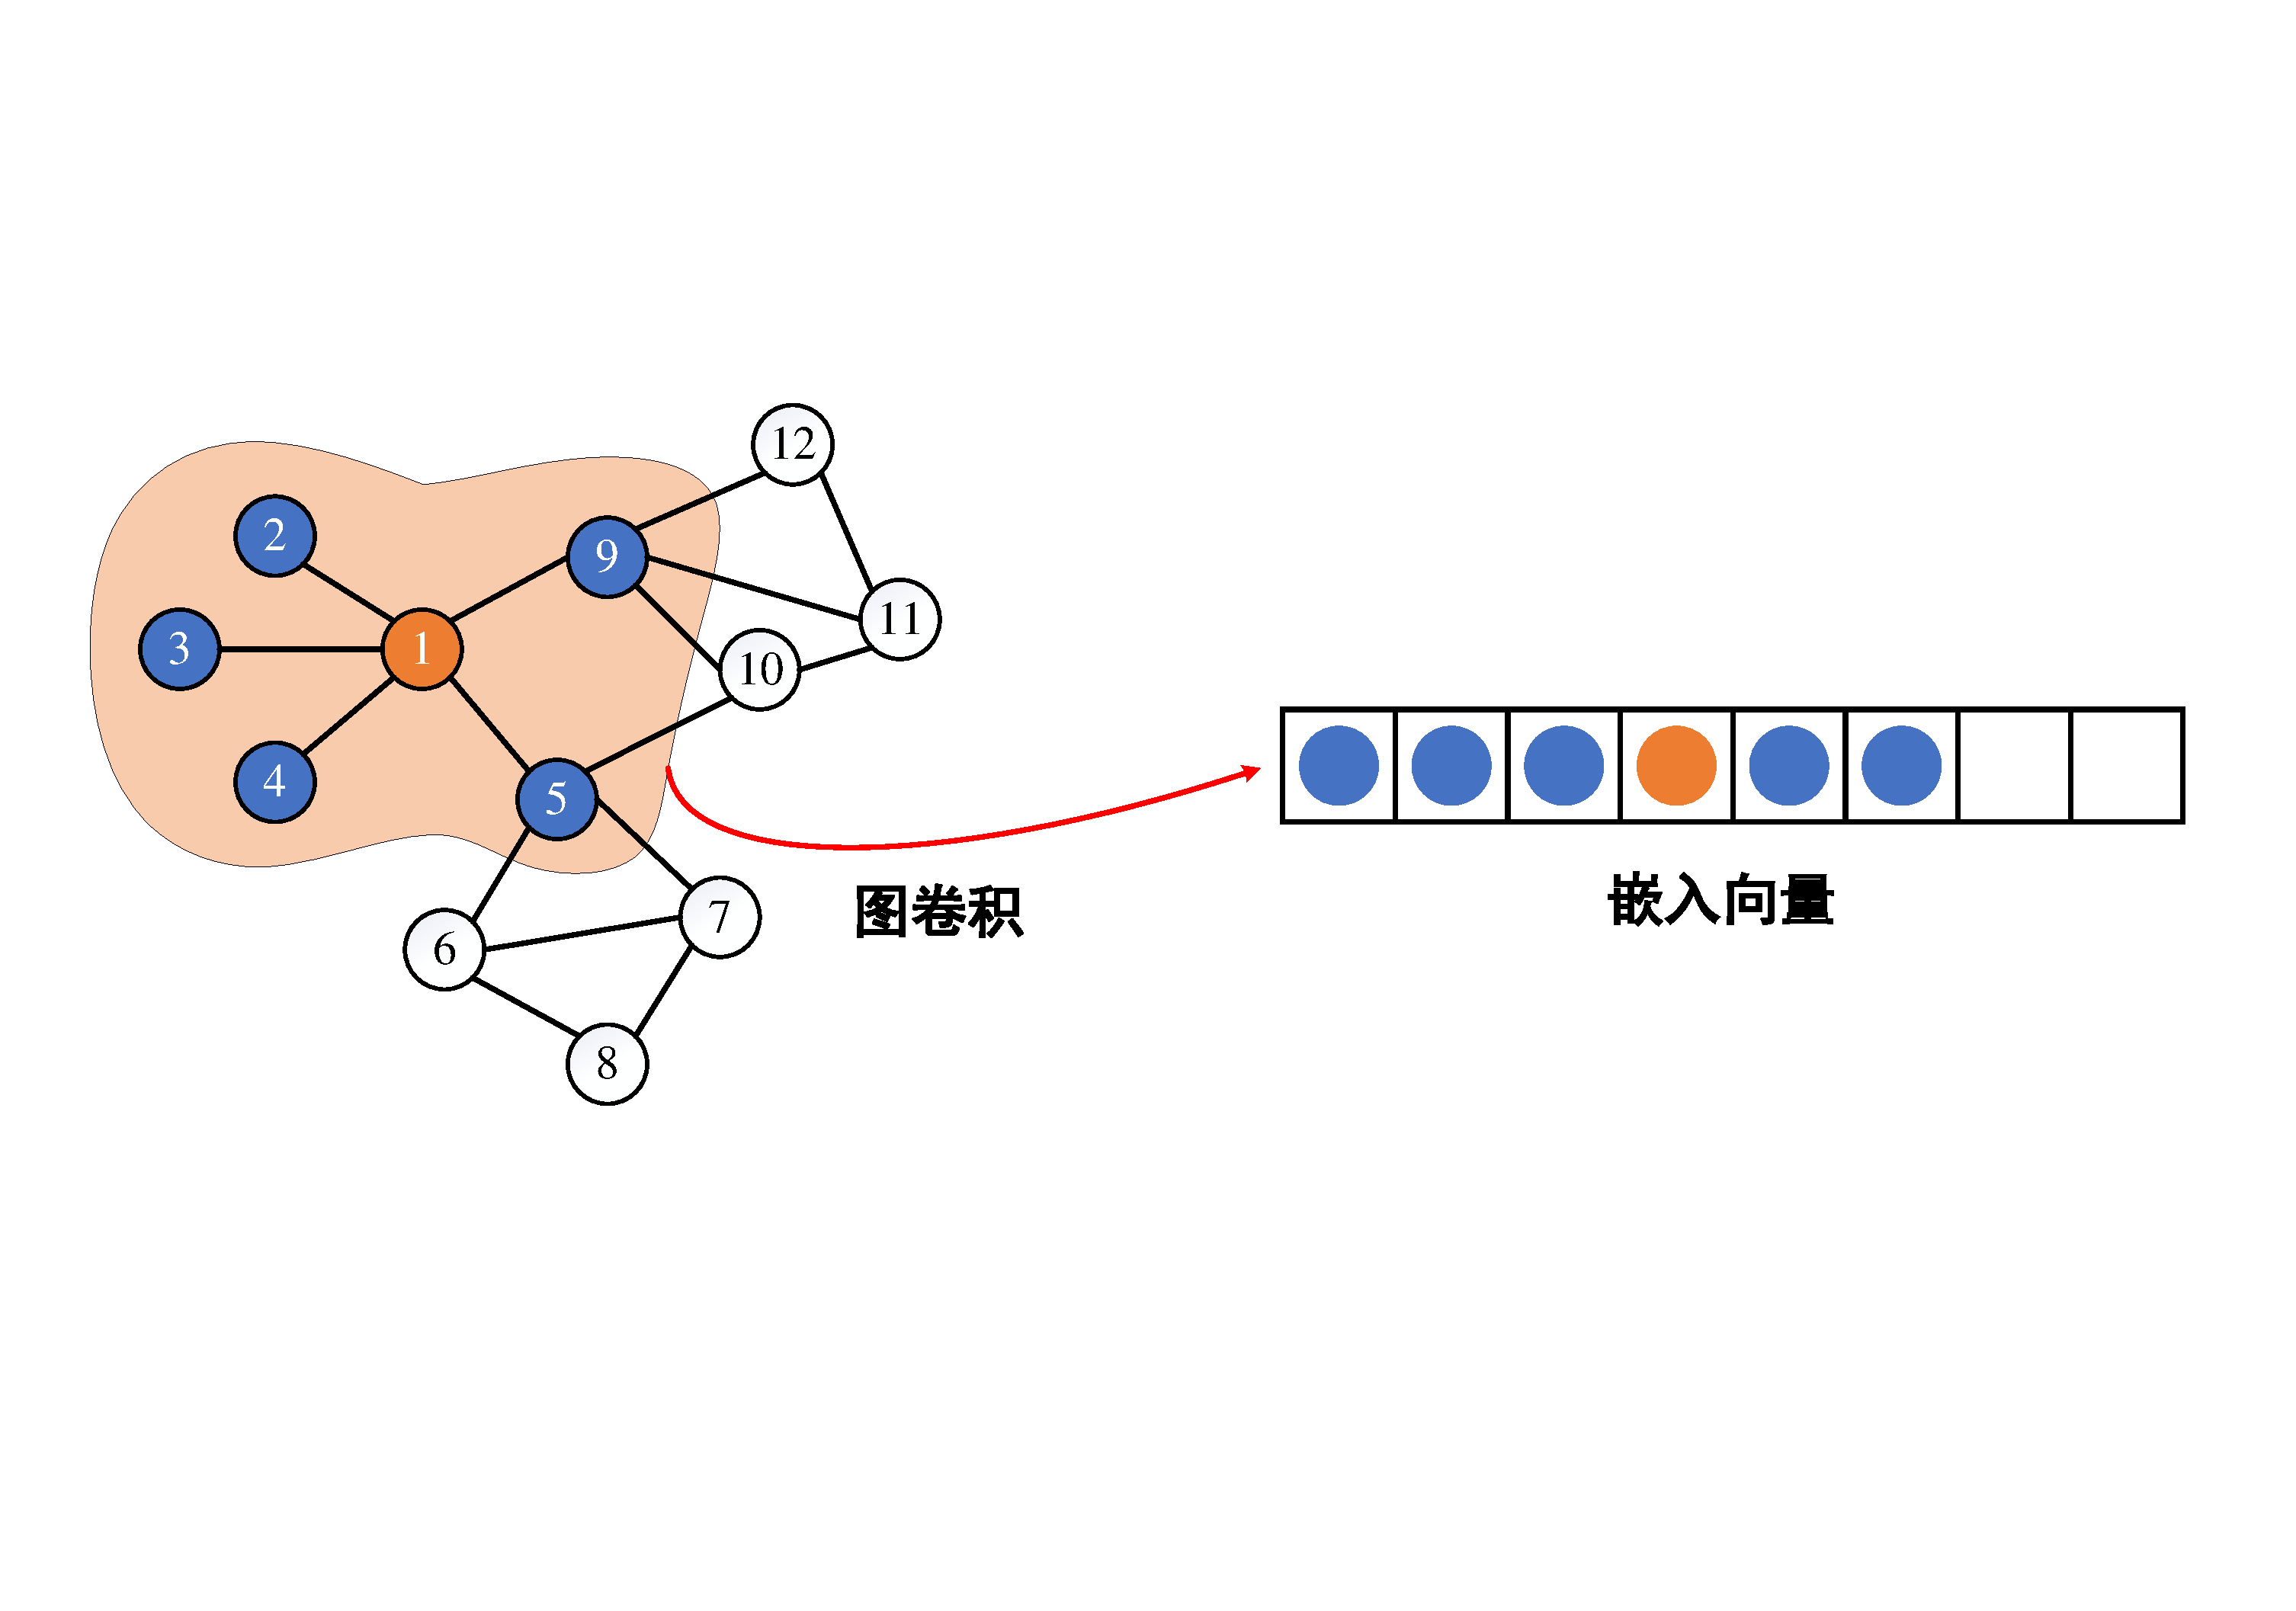
\includegraphics[scale=0.2]{./pic/gcn.pdf}
\caption{使用GCN生成路网节点嵌入}
\label{Figure.4.2.3}
\end{figure}

使用生成的路网节点嵌入表示作为道路节点信息$road_t$,使用GCN提取路网图空间结构特征和用户分布特征后的整体模型架构,通过STGRU层和GCN层的堆叠来实现。路网中的节点由向量表示,且会生成不同为维度特征向量。将输入向量定义为$X\in \mathbb{R}^{n \times C_i}$,输出向量维度定义为$C_o$。于是$road_t$的计算公式修改为:
\begin{equation}
   road_t = \sum\limits_{i=1}^{C_i} \Theta_{i,j}(L)x_i \in \mathbb{R}^n, 1 \leqslant j \leqslant C_o
\end{equation}
其中$X$为$t$时刻轨迹点所在的路网节点。

\section{实验与分析}
本节首先设计多组对比实验和消融验证了本章提出的空间特征增强方法以及各模块的有效性,然后通过应用分析得到不同长度数据在聚集预测任务中的性能表现。

\subsection{实验配置}
本章所使用的实验环境配置、数据集、评价指标以及基线方法均第三章一致,详见章节\ref{实验配置}。

\subsection{对比实验}
\textbf{方法比较。}表\ref{Table.4.1}中给出了SEGPM模型、STGRU模型和六个基线模型在三个数据集上的性能表现。在对比实验中,所使用的参数设置参照章节\ref{对比实验设置}所示,GCN嵌入向量维度设置为8,目的是维持模型参数量的一致性,减少由参数量变化带来的影响。
\begin{table*}[!ht]
\centering
\caption{SEGPM与基线模型在三个数据集上Recall@K和AUC指标的结果}%添加标题 设置标签
\label{Table.4.1}
\setlength{\tabcolsep}{5mm}{
\begin{tabular}{cccccc}% 通过添加 | 来表示是否需要绘制竖线
\toprule[1.5pt]  % 在表格最上方绘制横线
\textbf{NPF}  & recall@1 & recall@5 & recall@10 & recall@20 & AUC\\
\midrule[0.75pt]
LSTM    & 0.0428   & 0.1677   & 0.2894    & 0.4300    & 0.6951 \\

GRU     & 0.0712   & 0.2372   & 0.3421    & 0.4771    & 0.7778 \\

RNN     & 0.0809   & 0.2580   & 0.3570    & 0.4865    & 0.8018 \\

ST-LSTM & 0.0621   & 0.2438   & 0.3663    & 0.5050    & 0.7976 \\

STGN    & 0.0762   & 0.2728   & 0.3734    & 0.5061    & 0.8177 \\

STGRU   & 0.0920   & 0.2829   & 0.3891   & 0.5231    & 0.8290 \\

SEGPM&\textbf{0.1002}&\textbf{0.2966}&\textbf{0.3936}&\textbf{0.5256}&\textbf{0.8413}\\
\bottomrule[1.5pt] % 在表格最下方绘制横线
\end{tabular}
\\
\centering
\begin{tabular}{cccccc}% 通过添加 | 来表示是否需要绘制竖线
\toprule[1.5pt]  % 在表格最上方绘制横线
\textbf{OPF}  & recall@1 & recall@5 & recall@10 & recall@20 & AUC\\
\midrule[0.75pt]
LSTM    & 0.0383 & 0.1638 & 0.2634 & 0.4375 & 0.7140 \\

GRU     & 0.0455 & 0.1979 & 0.3007 & 0.4656 & 0.7611 \\

RNN     & 0.0588 & 0.2258 & 0.3260 & 0.4881 & 0.8324 \\

ST-LSTM & 0.0502 & 0.2107 & 0.3174 & 0.4890 & 0.7817 \\

STGN    & 0.0633 & 0.1699 & 0.2833 & 0.4920 & 0.8292 \\

STGRU   & 0.0681 & 0.2439 & 0.3464 & 0.5116 & \textbf{0.8545} \\

SEGPM&\textbf{0.0835}&\textbf{0.2509}&\textbf{0.3542}&\textbf{0.5207}&0.8538\\
\bottomrule[1.5pt] % 在表格最下方绘制横线
\end{tabular}
\\
\centering
\begin{tabular}{cccccc}% 通过添加 | 来表示是否需要绘制竖线
\toprule[1.5pt]  % 在表格最上方绘制横线
\textbf{TPF}  & recall@1 & recall@5 & recall@10 & recall@20 & AUC\\
\midrule[0.75pt]
LSTM    & 0.0752 & 0.3331 & 0.4849 & 0.6428 & 0.8317 \\

GRU     & 0.0789 & 0.3319 & 0.4793 & 0.6384 & 0.8451 \\

RNN     & 0.0856 & 0.3634 & 0.5066 & 0.6561 & 0.8645 \\

ST-LSTM & 0.0864 & 0.3699 & 0.5213 & 0.6682 & 0.8727 \\

STGN    & 0.0900 & 0.3327 & 0.5103 & 0.6672 & 0.8734 \\

STGRU   & 0.0933 & 0.3795 & 0.5263 & 0.6730 & 0.8755 \\

SEGPM&\textbf{0.1090}&\textbf{0.4060}&\textbf{0.5589}&\textbf{0.6993}&\textbf{0.8804}\\
\bottomrule[1.5pt] % 在表格最下方绘制横线
\end{tabular}}
\end{table*}

如表中实验结果所示,本章提出的SEGPM模型在三个数据集上的绝大多数指标均优于基线模型。在NPF、OPF、TPF三个数据集上,SEGPM模型$Recall@1$指标的提升依次为8.9$\%$ - 134.1$\%$,22.6$\%$ - 118$\%$和16.8$\%$ - 44.9$\%$。实验结果表明,SEGPM模型中对路网结构进行嵌入表示以及基于希尔伯特曲线的标签生成方法能够大幅提升模型建模时空特征的能力以及对聚集预测任务的有效性。因为这两种方式均有效增强了模型的时空特征提取能力,带来了一定的性能提升。同时路网结构的嵌入表示中考虑了用户之间的分布特征,提升了聚集预测建模多用户行为模式的能力。

基于希尔伯特曲线的标签生成方法保留了标签之间的空间特征,极大程度降度了标签数值之间的稀疏性问题,大幅降度了SEGPM模型对标签数值拟合的复杂度。对单用户进行建模的轨迹预测模型难以考虑到对应的其余用户的分布对用户行为模式的影响,在聚集预测任务中并不完全适用。路网结构嵌入时考虑了用户的分布情况,能够更准确的建模多用户场景下的行为模式。基于空间特征增强的聚集预测模型能够有效地对多用户之间的相互影响。

\subsection{消融实验}
为了验证本章提出的使用希尔伯特曲线的标签生成方法和基于GCN的路网结构嵌入方法的有效性,本节设置了两组使用单个方法的消融实验,并在三个数据集上进行实验,实验结果如表\ref{Table.4.2}所示。其中$\mathrm{STGRU}_1=STGRU+HC$为仅使用希尔伯特曲线进行区域编号,$\mathrm{STGRU}_2=STGRU+GCN$表示仅使用GCN生成路网图的节点嵌入。
\begin{table*}[!ht]
\centering
\caption{路网特征嵌入和标签特征增强对模型性能的影响}%添加标题 设置标签
\label{Table.4.2}
\setlength{\tabcolsep}{5mm}{
\begin{tabular}{lccccc}
\toprule[1.5pt]  % 在表格最上方绘制横线
\textbf{NPF}  & recall@1 & recall@5 & recall@10 & recall@20 & AUC\\
\midrule[0.75pt]
STGN    & 0.0762   & 0.2728   & 0.3734    & 0.5061    & 0.8177 \\

STGRU   & 0.0920   & 0.2829   & 0.3891    & 0.5231    & 0.8290 \\

$\mathrm{STGRU}_1$& 0.0974   & 0.2867   & 0.3881    & 0.5161    & 0.8356 \\

$\mathrm{STGRU}_2$& 0.0968   & 0.2881   & 0.3891    & 0.5179    & 0.8259 \\

SEGPM&\textbf{0.1002}&\textbf{0.2966}&\textbf{0.3936}&\textbf{0.5256}&\textbf{0.8413}\\
\bottomrule[1.5pt]
\end{tabular}
\\
\centering
\begin{tabular}{lccccc}
\toprule[1.5pt]  % 在表格最上方绘制横线
\textbf{OPF}  & recall@1 & recall@5 & recall@10 & recall@20 & AUC\\
\midrule[0.75pt]
STGN    & 0.0633 & 0.1699 & 0.2833 & 0.4920 & 0.8292 \\

STGRU   & 0.0681 & 0.2439 & 0.3464 & 0.5116 & \textbf{0.8545} \\

$\mathrm{STGRU}_1$& 0.0819   & 0.2436   & 0.3516    & 0.5193    & 0.8519 \\

$\mathrm{STGRU}_2$& 0.0700   & 0.2458   & 0.3516    & 0.5158    & 0.8542 \\

SEGPM&\textbf{0.0835}&\textbf{0.2509}&\textbf{0.3542}&\textbf{0.5207}&0.8538\\
\bottomrule[1.5pt]
\end{tabular}
\\
\centering
\begin{tabular}{lccccc}
\toprule[1.5pt]  % 在表格最上方绘制横线
\textbf{TPF}  & recall@1 & recall@5 & recall@10 & recall@20 & AUC\\
\midrule[0.75pt]
STGN    & 0.0900 & 0.3327 & 0.5103 & 0.6672 & 0.8734 \\

STGRU   & 0.0933 & 0.3795 & 0.5263 & 0.6730 & 0.8755 \\

$\mathrm{STGRU}_1$& 0.1010   & 0.3780   & 0.5326    & 0.6646    & 0.8783 \\

$\mathrm{STGRU}_2$& 0.1039   & 0.3776   & 0.5308    & 0.6651    & \textbf{0.8835} \\

SEGPM&\textbf{0.1090}&\textbf{0.4060}&\textbf{0.5589}&\textbf{0.6993}&0.8804\\
\bottomrule[1.5pt]
\end{tabular}}
\end{table*}

由实验结果可知,本章提出的使用希尔伯特曲线和GCN嵌入增强STGRU模型的空间特征方法在三个数据集的绝大多数指标上取得了较为明显的提升。以Recall@1指标为例,STGRU+HC+GCN模型相较于基线模型STGN模型性能提升分别为5.2$\%$ - 27.03$\%$,22.6$\%$ - 31.9$\%$和16.8$\%$ - 21.1$\%$。结果表明,单独使用希尔伯特曲线生成区域编号或GCN生成路网图的节点嵌入,均能够较好的增强对数据集中空间特征的增强。同时考虑上述两者时的模型性能提升较为明显。

且在不同数据集上两者的性能提升有所差别。在NPF和OPF数据集中,使用希尔伯特曲线的性能提升相较于路网图节点嵌入更大,原因是这两个数据集中用户数量较少,轨迹点较为稀疏,路网图节点嵌入对整体用户行为模式的建模影响较小。路网图中包含了当前分户分布信息,较为稀疏的轨迹点分布对建模多用户之间的行为模式的影响减弱。而TPF数据集中轨迹点分布更加密集,用户分布情况的建模对当前用户的行为模式影响较大,因此使用路网图节点嵌入的STGRU模型性能较仅增强区域编号之间的空间特征有更好的性能表现。

两种方法同时使用的性能表现优于单独考虑其中一种方法。这是因为使用希尔伯特曲线进行区域编号能够增强预测区域间的空间特征,更有助于提升$Recall@1$性能。在OPF数据集上体现的较为明显,$STGRU_1$和$STGRU_2$在其余指标上相差无几,但$STGRU_1$的$Recall@1$提升了20.3$\%$,提升十分明显。而使用GCN模型生成路网图节点嵌入与长短期路网特征的提取相结合,能够更好的提取用户之间的时空特征,建模多用户场景下的用户行为模式。两种方法对模型性能提升的作用域重叠较少,几乎不存在性能相互抵消或冲突的现象,因此同时考虑两种方法能够相较于单独使用任一方法均有所提升。

\textbf{向量维度影响。}图卷积网络生成节点嵌入向量的维度对的嵌入表示的性能影响较大,于是设置了使用不同维度节点嵌入向量的STGRU+GCN模型进行实验,通过生成并使用不同维度的节点嵌入为$8,16,32,64$来完成。从表\ref{Table.4.2}可以发现,随着向量维度的增加各项性能指标均有所提升。当向量维度增加到64时,出现了性能的整体下滑,且下降明显,原因是当向量维度较大时,路网门控结构不能很好的提取和建模向量中的路网结构特征,甚至有一定程度的反作用。
\begin{table}[!ht]
\centering
\caption{使用不同维度节点嵌入向量的性能}
\label{Table.4.2}
\setlength{\tabcolsep}{1mm}{
\begin{tabular}{ccccc}% 通过添加 | 来表示是否需要绘制竖线
\toprule[1.5pt]  % 在表格最上方绘制横线
\textbf{}vector dimension  & recall@1 & recall@5 & recall@10 & recall@20 \\
\midrule[0.75pt]
8    & 0.1039 & 0.3776 & 0.5308 & 0.6651\\

16     & 0.1054 & 0.3757 & 0.5300 & 0.6707\\

32     & \textbf{0.1081} & \textbf{0.3903} & \textbf{0.5405} & \textbf{0.6800} \\

64 &   0.1037 &  0.3806  &  0.5387   & 0.6735 \\
\bottomrule[1.5pt]
\end{tabular}}
\end{table}

\subsection{应用分析}
聚集预测对轨迹数据的质量要求较高,在分布时间相同的轨迹中,不同轨迹长度对建模用户行为模式影响较大。本小节通过设置不同长度的轨迹数据进行实验,一共在三个数据集上设置了14组实验,所使用的轨迹长度分别为$(0,50)$、$[50,100)$、$[100,150)$、$[150,200)$以及$[200,\infty)$。由于NPF数据集中长度在200以上的数据极少,因此在NPF数据集上仅设置了4组实验,其余两个数据集上均为5组实验。
\begin{figure}[!ht]
\centering
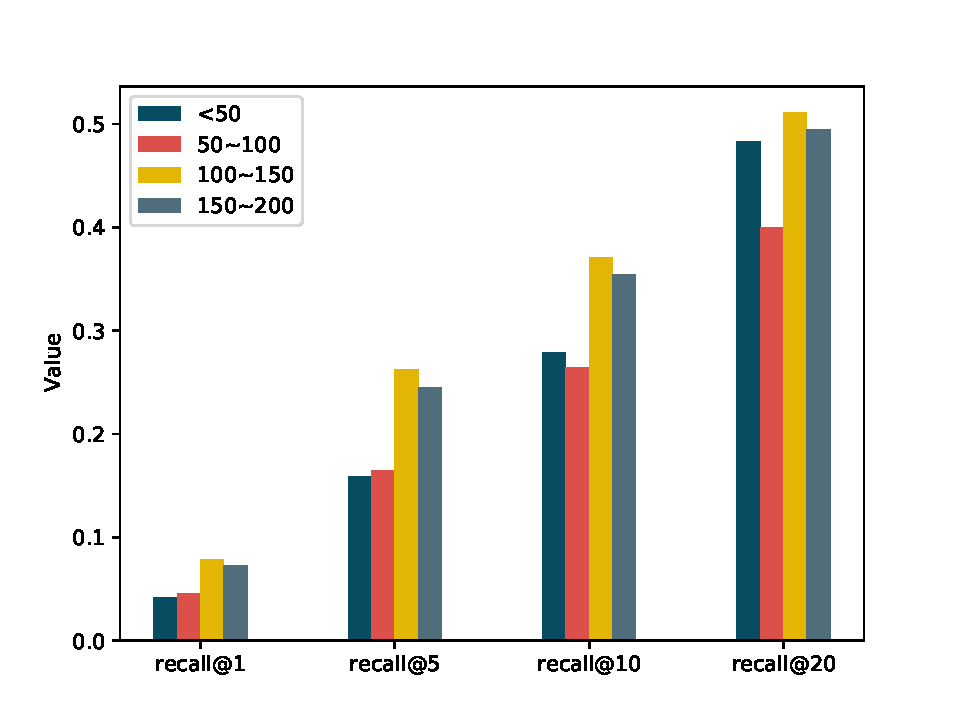
\includegraphics[scale=0.41]{./pic/figure-4-c.pdf}
\caption{NPF中的性能表现}
\label{Figure.4.2.5}
\end{figure}
如图\ref{Figure.4.2.5}所示为基于NPF数据集的4组实验结果,实验设置与前文一致,评价指标为$recall@k$,其中$k=\{1,5,10,20\}$。在所有的四个指标上100~150区间和150~200区间的性能表现最好。此外,轨迹长度小于50时的性能表现较好,因为NPF数据集中该区间的轨迹数据较少,大大降低了建模难度。
\begin{figure*}[!ht]
\centering 
\begin{minipage}[b]{0.45\linewidth}
\centering
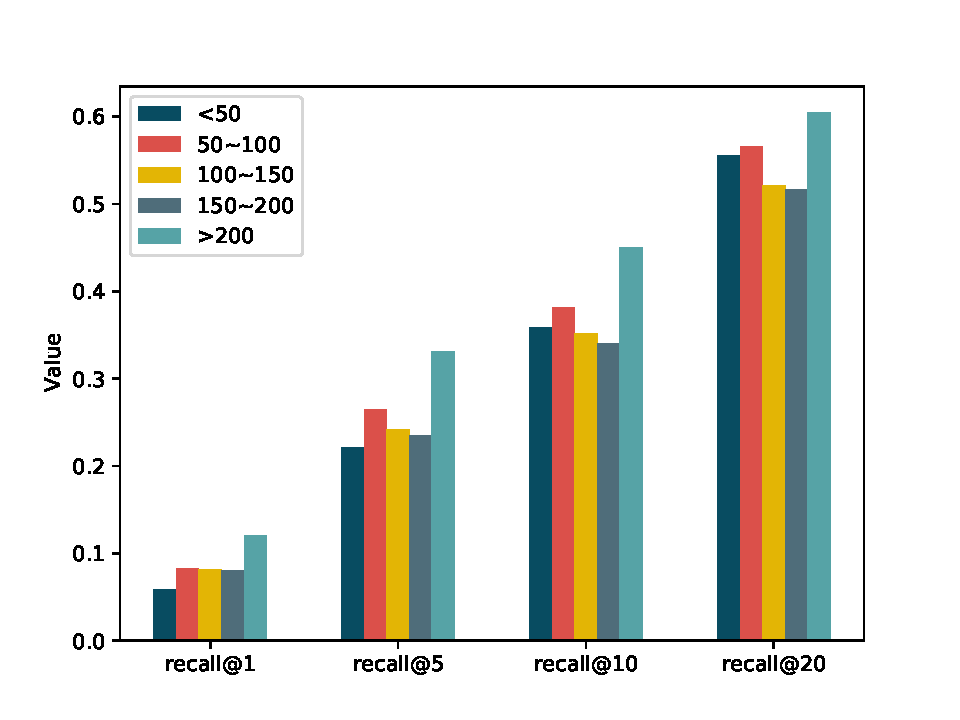
\includegraphics[width=0.98\linewidth]{./pic/figure-4-k.pdf}
\caption{OPF中的性能表现}
\label{Figure.4.2.6}
\end{minipage}
\begin{minipage}[b]{0.45\linewidth} 
\centering 
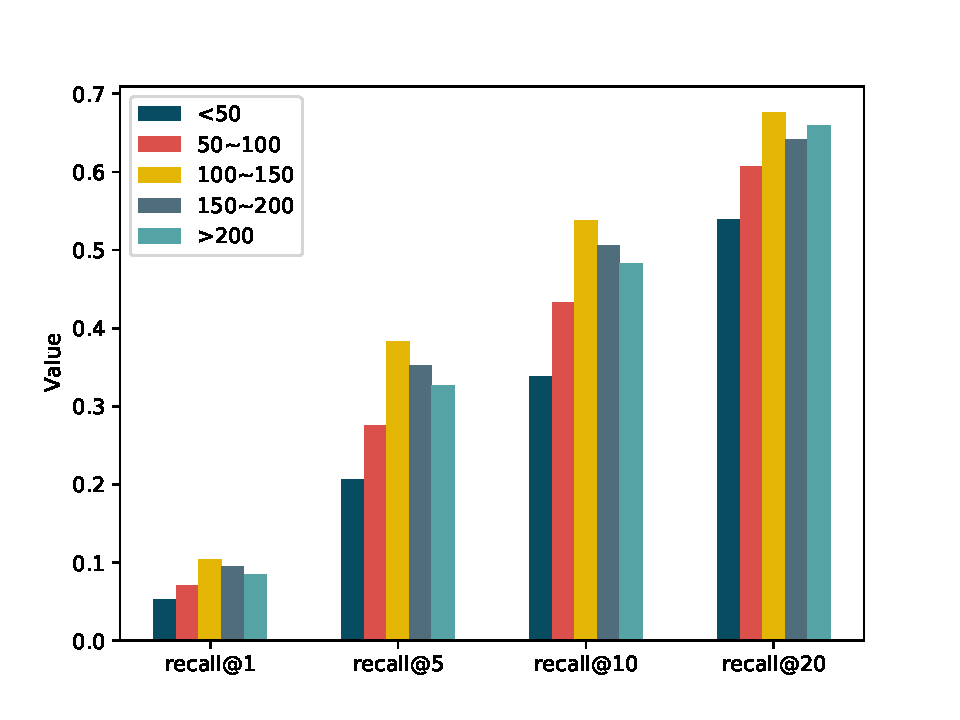
\includegraphics[width=0.98\linewidth]{./pic/figure-4-t.pdf}
\caption{TPF中的性能表现}
\label{Figure.4.2.7}
\end{minipage}
\end{figure*}

如图\ref{Figure.4.2.6}所示为OPF数据集上的5组实验结果,其中性能表现最好的区间为50~100,其余区间稍弱。在轨迹长度大于200时性能指标高于前文中对比实验的结果,同样为数据量较少所致。

最后是在TPF数据集上的实,如图\ref{Figure.4.2.7}所示,性能表现从高到低分别为100~150区间、150~200区间、大于200区间、50~100区间和小于50区间。其中轨迹长度大于200的$recall@20$指标仅低于100~150区间,说明了轨迹长度对粗粒度的预测结果存在正向驱动。

综合上述实验,相同分布时间的不同长度的轨迹数据意味着完全不同的行为模式以及样本质量,如果用户的轨迹较短,意味着该用户的移动次数较少,虽然在建模用户行为模式时较为困难,但这类用户更偏向于在某处长期停留,对整体结果影响较小。反之当用户轨迹过长时,模型精度并不足以对其意图进行精确预测,反而会对整体的聚集预测造成影响。因此在聚集预测中,使用移动次数较多并且由一定停留的轨迹数据更容易进行预测。

\section{本章小结}
在本章中,通过增强轨迹数据中的空间特征,在第三章STGRU模型的基础上提出了一个聚集预测模型。在聚集预测模型中,融合了希尔伯特曲线增强标签之间的空间特征和;然后引入图嵌入结构建模路网图的结构信息以及用户之间的相互影响,这对于建模多用户行为模式有很大的帮助;使用希尔波特曲线增强区域标签能够增强标签之间的语义关系,降低模型建模的难度;图嵌入结构所生成的向量作为输入的一部分并通过路网门控进行建模,且其中包含了用户之间的分布信息,能够建模用户在不同用户分布情况下的行为模式。最后在三个真实世界的数据集上进行多项实验验证聚集预测模型的有效性,它在第三章STGRU模型的基础上取得了较好的性能提升。

\chapter{基于城市流量的聚集预测告警系统实现}
为了帮助更好的掌握城市中的聚集情况,为城市中对聚集情况的管理管控提供支撑,本章介绍了聚集预测告警系统的设计与实现,并进行了功能和性能测试。

\section{引言}
随着智慧城市建设的推进和各类智能设备的推广,城市管理部门能够采集到用户在公共场所的位置信息与日俱增,这些数据中包含用户的移动轨迹、分布情况等。在人口密集的现代化城市中,由于人口聚集导致的各类恶性事件是城市管理者一直面临的难题。在人工智能、大数据技术不断发展的当下,如何利用好这些数据帮助城市管理者掌握城市中的聚集情况并基于此做出合理反映,能够极大程度提升城市的管理管控能力。在该任务中,如何提取数据中的时空特征对用户行为模式进行建模,实现更精确的用户位置预测是需要解决的核心问题。

在本文三、四章中提出的聚集预测模型的基础上,结合实际场景下的轨迹数据分析和聚集预测需求,本章实现了基于城市流量的聚集预测告警系统的设计与开发。首先,结合任务进行需求分析和系统的整体设计。然后,简单介绍了系统的实现,并通过可视化方案对系统的功能和界面布局进行展示。最后,对系统的功能和性能进行了测试。

\section{系统概述}
本章中设计实现的聚集预测告警系统整体采用B/S架构,web端开发及UI设计基于HTML5、CSS3和Kepler.gl库实现,后端采用python的Falsk框架,相关服务部署环境如表\ref{Table.3.1}所示,数据库采用SQLite。主要开发工具为Microsoft公司的Visual Studio Code软件。

基于城市流量的聚集预测告警系统在前两章所提出的聚集预测模型上进行开发,主要面向的是城市场景下的聚集预测问题。系统包括数个前端界面、一个由Flask和SQLite实现的后端数据处理程序以及一个基于tensorflow的模型实现,基于Uinx操作系统开发实现。

\section{需求分析}
本节对聚集预测告警系统进行简单的需求分析,并通过系统用例图和数据流图进行需求建模分析。该系统需要实现数据展示和基于模型推理的聚集预测结果呈现,对其进行分析后绘制了如图\ref{Figure.5.1}所示为聚集预测告警系统的系统用例图,主要用例为数据选择、数据处理、数据传输、聚集预测、数据存储和结果展示等。
\begin{figure}[!ht]
\centering
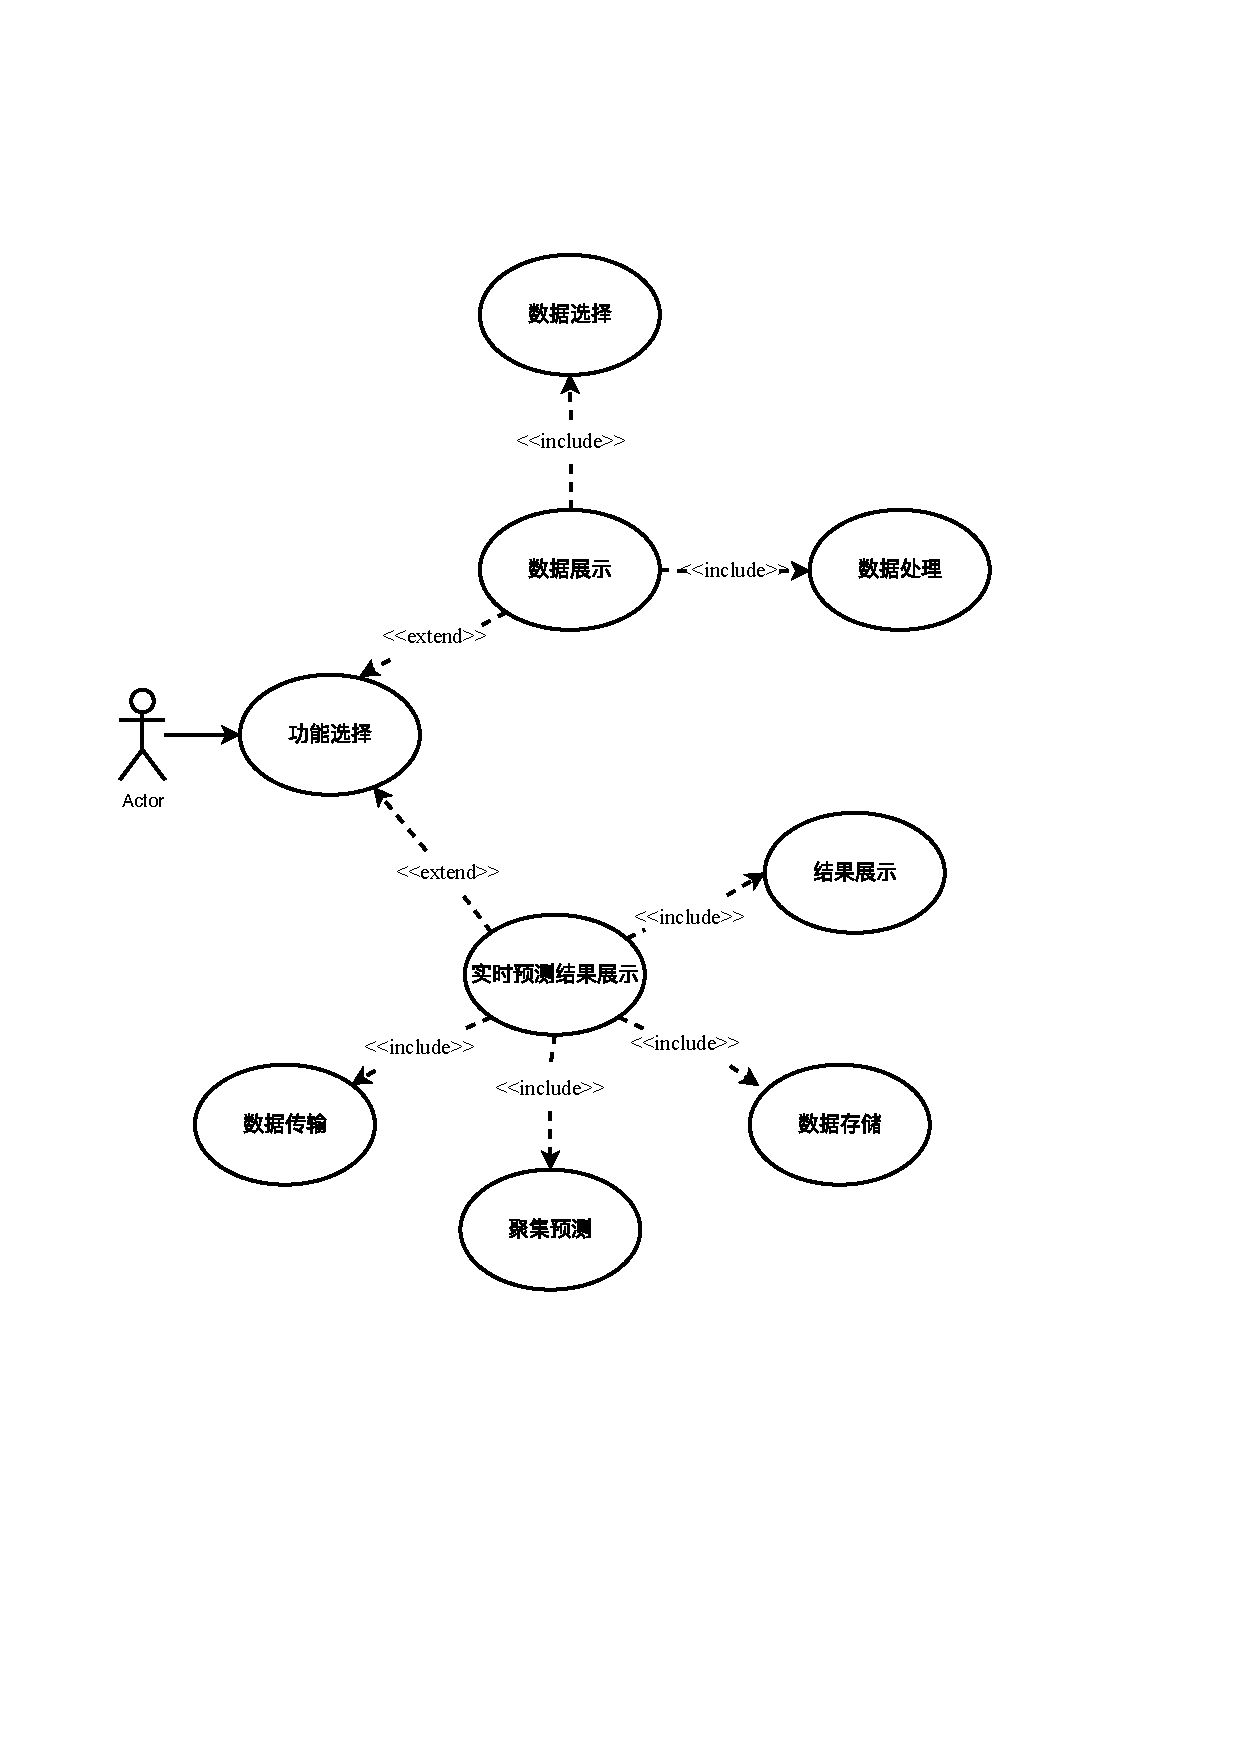
\includegraphics[scale=0.7]{./pic/用例图.pdf}
\caption{聚集预测告警系统用例图}
\label{Figure.5.1}
\end{figure}

如图\ref{Figure.5.2}所示为经过分析后得到的本系统数据流图。其中的数据展示事务,主要由资源管理模块对用户所选择的关键字通过数据库查询得到对应的轨迹数据和路网数据,然后根据预设的模型在前端界面上进行展示,并支持用户对数据的可视化交互。对于聚集预测结果展示事务,资源管理模块控制数据传输接口的开放,数据传输和处理模块实时接收并结合历史轨迹信息生成样本,样本数据由聚集预测模块进行预测推理,所得到的结果在前端界面上进行展示,同时将预测结果存入数据库中。本章开发的聚集预测告警系统功能主要包括:

(1)对用户选择的轨迹数据和路网数据进行可视化展示。 

(2)实时接收移动端传输的数据。

(3)实现对实时数据进行聚集预测。

(4)对实时数据和预测结果进行可视化展示。

(5)将轨迹数据和预测结果存入数据库。

(6)在前端界面中提供可视化交互能力。

在性能需求方面,本章提出的聚集预测告警系统需要满足同时接收多设备数据,模型推理耗时应在小于轨迹采样的时间间隔(通常为5分钟),且聚集预测的结果需要达到一定精度。

\begin{figure}[!ht]
\centering
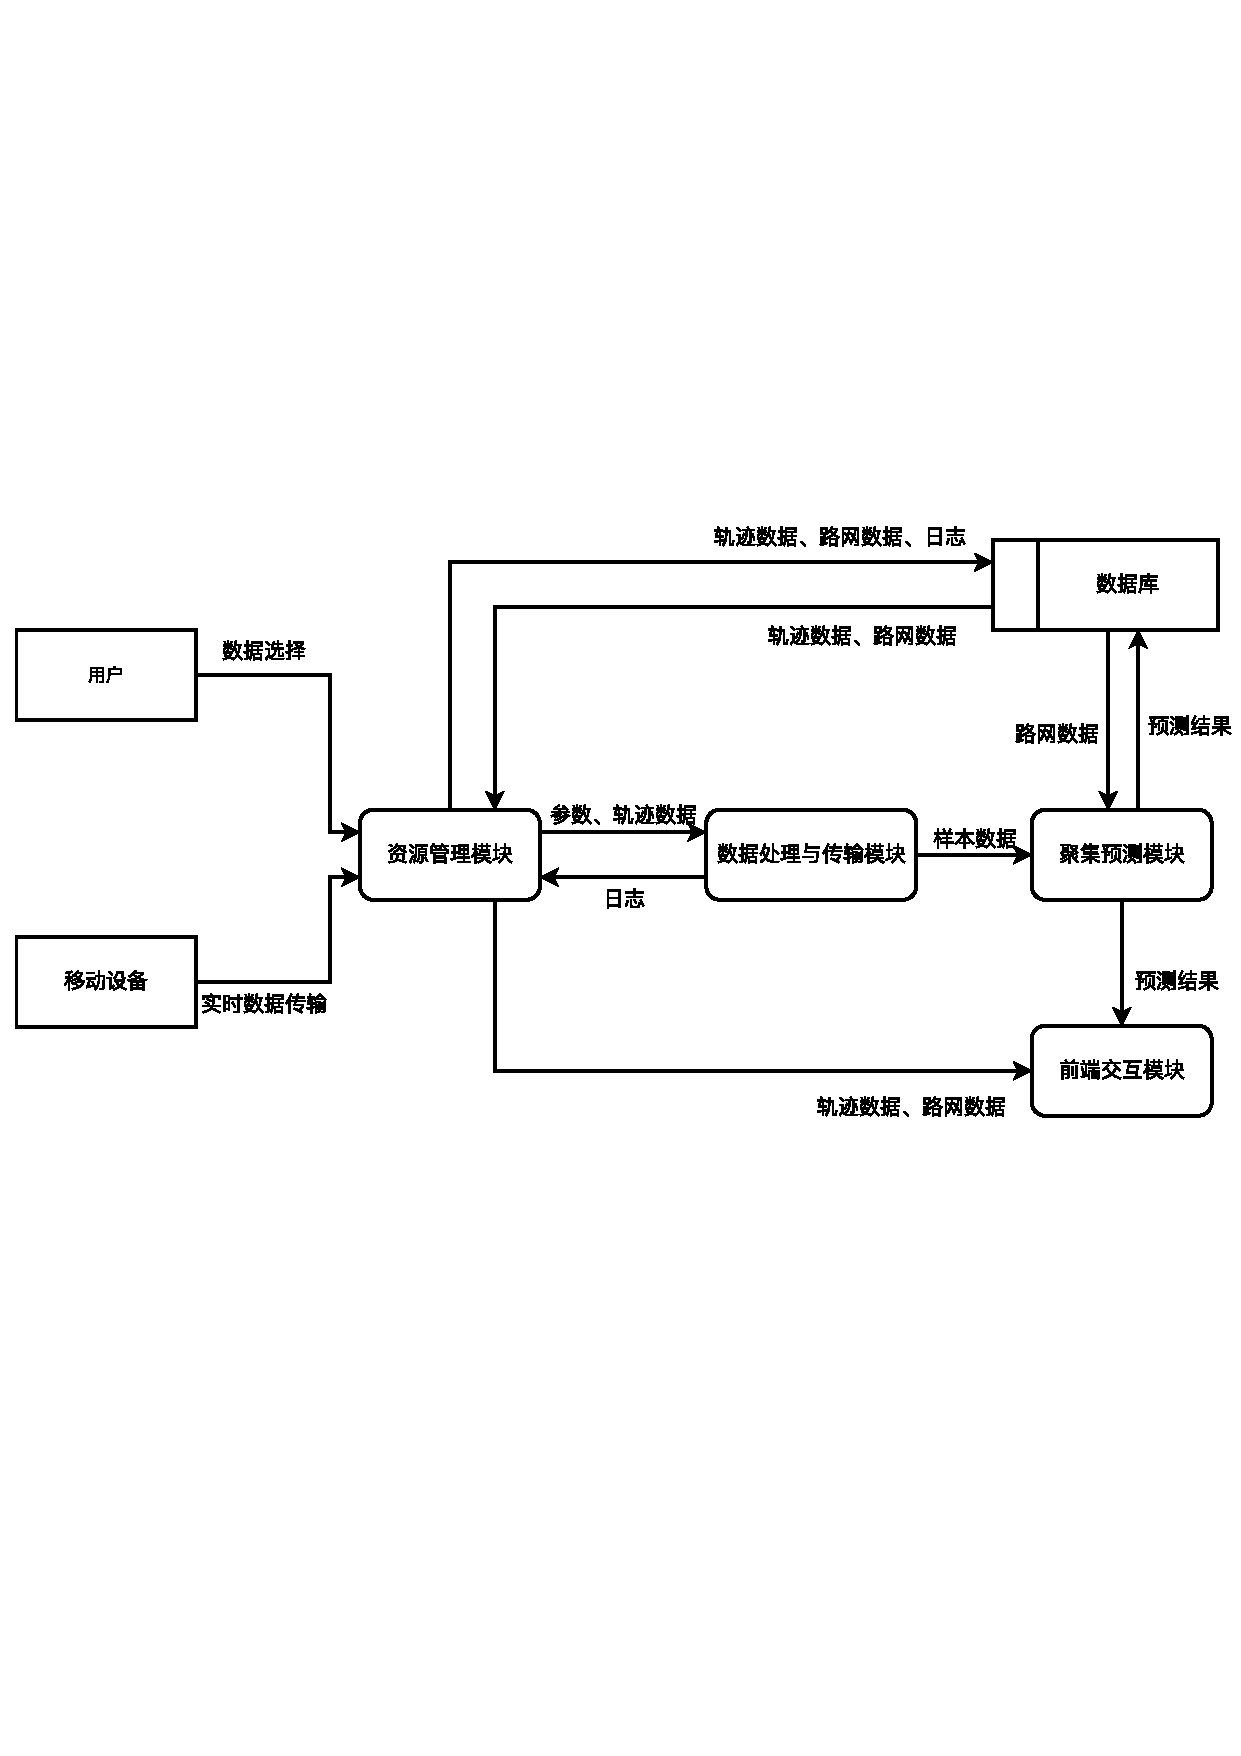
\includegraphics[width=1.0\linewidth]{./pic/数据流图.pdf}
\caption{聚集预测告警系统数据流图}
\label{Figure.5.2}
\end{figure}

聚集预测告警系统整体为四层架构,分别为表现层、业务层、服务层和数据库。其中表现层主体为UI界面,基于HTML5和CSS3语言开发,在页面中通过基于Flask的Dash框架嵌入了Uber公司开发的Kepler.gl库实现简单的交互能力;业务层包括计算资源调度、数据处理和异常处理,实现了除聚集预测模型外的所有计算功能;服务层主要提供对外的输出传输接口和模型调用接口,实现基于移动终端设备的试试数据获取以及充分利用远程计算资源;数据库中主要存储系统所产生的日志信息、历史轨迹信息以及路网结构信息;

从功能划分角度出发,系统主要包含四个功能模块,如图\ref{Figure.5.4}所示,分别是资源管理模块、数据传输和处理模块、聚集预测模块以及前端交互模块。
\begin{figure}[!ht]
\centering
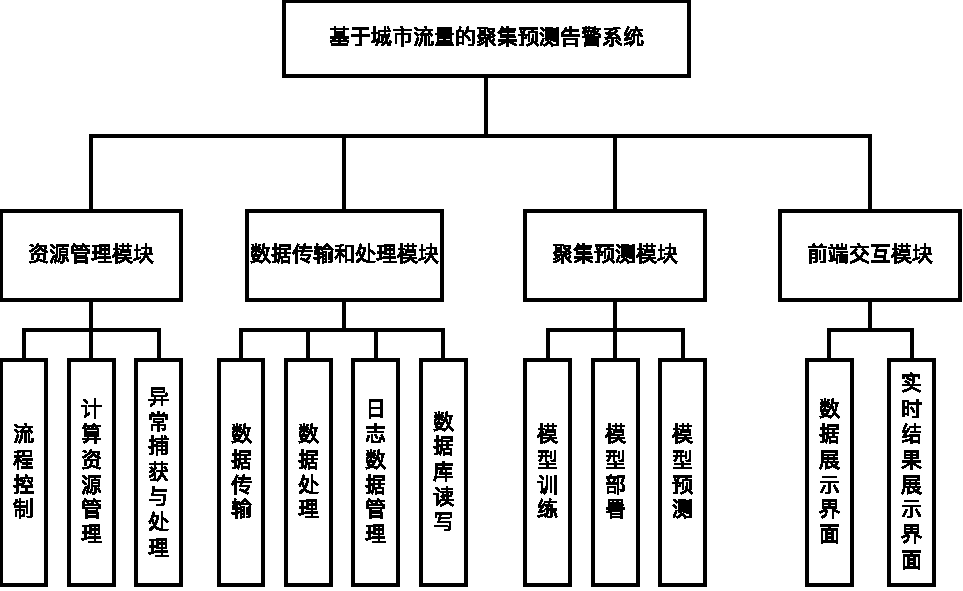
\includegraphics[width=1.0\linewidth]{./pic/模块图.pdf}
\caption{聚集预测告警系统模块图}
\label{Figure.5.4}
\end{figure}

1、资源管理模块。主要包括流程控制、计算资源的管理、异常的捕获与处理,负责整个系统运行过程中的资源管理调度,保障系统的正常运行,并具备处理系统运行时可能发生的多种异常的能力。

2、数据传输和处理模块。包括数据传输、数据处理、日志数据管理和数据库读写等,其中数据传输主要为提供并运行数据接口,通过端口监听实现与移动终端之间的信息传输功能;以及在数据样本生成后通过模型调用接口与聚集预测模块进行交互;并且能够对其他本地数据进行统一管理。

3、聚集预测模块。该模块主要负责模型训练、模型部署、模型预测,以及与数据传输和处理模块之间进行交互。分为模型训练、模型调用和数据交互三个部分。

4、前端交互模块。主要包括UI界面的设计与实现以及通过嵌入Kepler.gl库提供简单的自主交互能力,包括数据展示界面和实时结果展示界面。在数据展示界面中分别展示了轨迹数据的分布以及路网结构;实时结果展示界面同时对实时轨迹信息以及经过模型预测的结果进行展示。

\section{系统实现}
本节根据前文所述的整体设计思路对每个模块进行了详细的介绍。
\subsection{资源管理模块}
\begin{figure}[!ht]
\centering
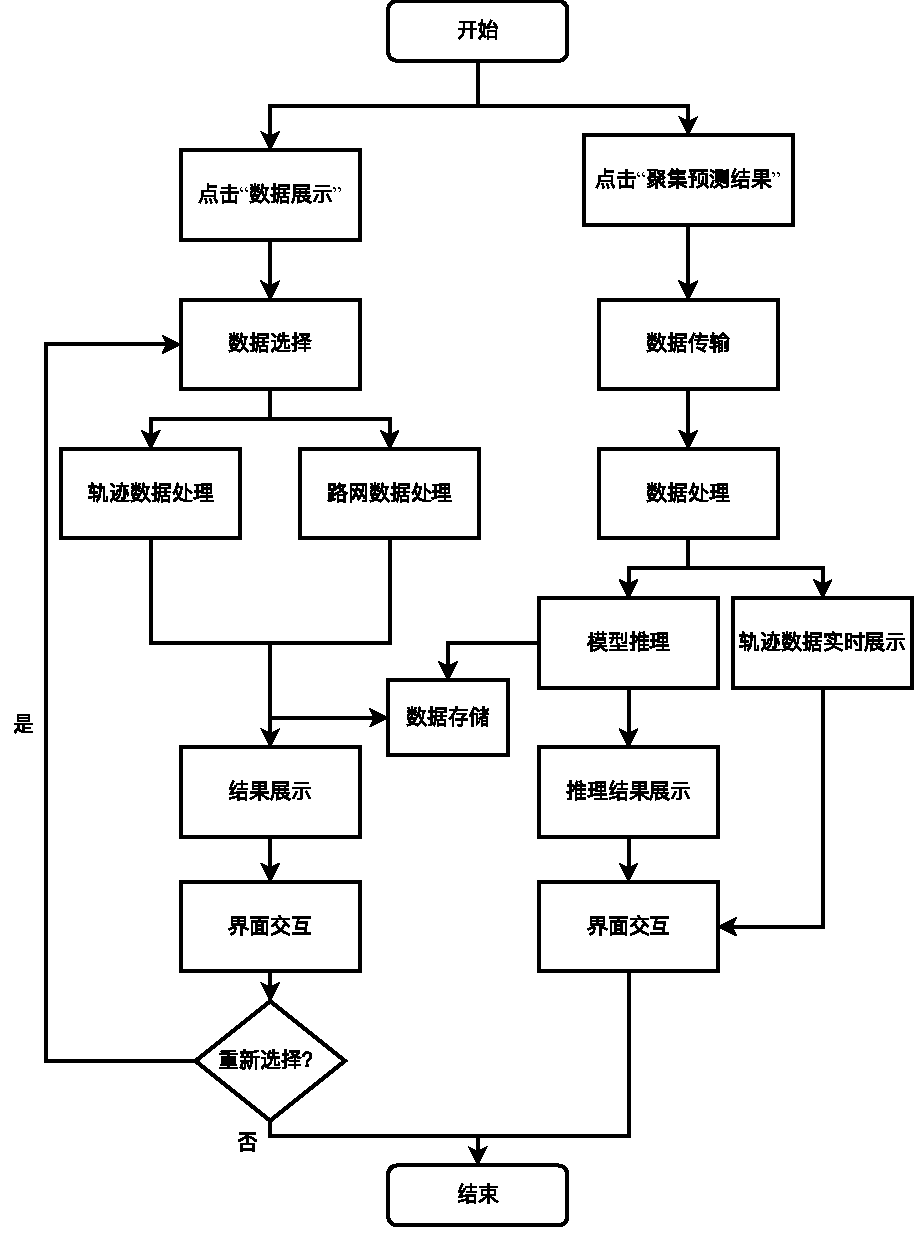
\includegraphics[scale=0.7]{./pic/流程图.pdf}
\caption{聚集预测告警系统整体流程图}
\label{Figure.5.5}
\end{figure}
资源管理模块是整个系统的管理中枢,为系统的运行提供保障。系统流程图如图\ref{Figure.5.5}所示,主要包含了对数据展示和聚集预测两个事务的管理。对于数据展示事务,基于用户选择的区域与轨迹数据,通过数据选择-数据处理-数据展示-界面交互的流程,对用户选择的轨迹数据的整体分布以及所处区域的路网结构的可视化信息通过两个Kepler.gl界面进行展示,并对路网结构进行了动态可视化。对于聚集预测事务,首先端口实时获取数据并对数据进行处理,通过调用部署的算法模型推理得到预测结果,同样在两个Kepler.gl界面中分别展示实时获取的轨迹信息以及处理后的聚集预测结果。

\subsection{数据传输和处理模块}
数据传输和处理模块主要负责数据传输、数据处理、日志数据管理和数据库读写。其中日志信息基于Logtail实现,主要记录系统的运行状态、用户操作、接口使用情况等。为后续系统使用中的bug进行溯源以及根据使用情况进行性能优化等。

对于实施数据的获取由数据传输接口实现,通过开放端口和端口监听获取移动端的位置信息和时间信息。并与部署模型的服务器之间构建了固定连接以传输处理好的轨迹数据并接收模型的预测结果。基于数据传输接口能够实现模型部署和系统部署的相互独立,对硬件要求更低,实际应用中部署更加灵活。

对与获取到的轨迹数据,需要结合路网图进行处理,以及对其进行样本划分以满足模型的输入要求,并提供了自主的参数设置能够满足不同场景下的应用需求。并将处理完的数据和模型推理结果在前端界面进行展示并存入数据库保存。

由于本系统中所涉及数据较为简单,同时为了降低系统部署端的计算资源需求,采用轻量化的开源数据库SQLite对数据进行存储。如表\ref{Table.5.1}所示为本文中所使用的数据库设计文档。
\begin{table*}[!ht]
\centering
\caption{数据库设计文档}%添加标题 设置标签
\label{Table.5.1}
\begin{tabular}{ccl}
\hline
字段& 存储类 & 描述\\
\hline
id& INTEGER &用户编号,根据传输设备自动生成\\
time& TIMESTAMP &时间戳信息\\
lat&  REAL &轨迹点纬度\\
lng& REAL &轨迹点经度\\
road& INTEGER &所处路段编号\\
label& INTEGER &所处区域编号\\
\hline
\end{tabular}
\end{table*}

\subsection{聚集预测模块}
聚集预测模块采用的是第四章中的基于空间特征增强的聚集预测模型,骨干网络为第三章中的时空门控循环单元(STGRU)。

在应用中首先需要对模型进行预训练,根据需要部署的区域获取对应的路网结构,并结合历史轨迹信息生成路网图。然后在对应的人流数据集上进行预训练,因为引入了路网结构知识,城市间的路网结构各不相同,不同城市数据集训练的模型在其他数据集上的泛化能力较差。

为了保证聚集预测结果的实时性,将模型部署在多张运算显卡上来增加数据吞吐量,大幅减少了模型推理部分的耗时。

\subsection{前端交互模块}
前端交互模块主要包含UI界面的设计与实现以及简单的自主交互能力。所有的UI设计使用侧边导航栏的方式,并将剩余空间均分为两部分以展示更多的内容并实现了一定的数据对比效果。事务切换通过侧边导航栏的NavLink组件实现.

\subsection{聚集预测结果展示界面}
用户点击【数据展示】可切换至数据展示界面,其中左侧为所选择数据的展示区域,数据通过Radio组件进行选择,右侧为对应区域的路网结构的展示区域,根据所选择数据自动适配。两个展示区域均基于Kepler.gl实现,支持简单的缩放、视角转换等功能,能够实现对数据进行全方位的展示。

点击【聚集预测结果】可切换至实时结果展示界面,此界面的数据传输与选择需在部署时进行配置。左侧为对实时获取的数据进行动态展示,右侧为根据模型预测结果进行聚集预测情况的可视化展示。

\section{系统展示}

\begin{figure}[!ht]
\centering
\includegraphics[width=1.0\linewidth]{./pic/聚集预测结果展示界面.png}
\caption{聚集预测结果展示界面}
\label{Figure.5.8}
\end{figure}

通过系统部署服务器的IP地址和设置的web服务端口可以在任意浏览器中访问本系统。进入本系统时,默认进入数据展示界面,加载为【day1】标签所对应的数据。右侧加载对应的路网数据,并通过模拟时间戳实现了动态展示。可以通过对顶部Radio组件选择不同时间的历史数据,轨迹数据展示部分和路网数据展示部分会同时重新加载对应的轨迹数据和路网数据。当用户处于其他界面时,可以通过点击侧边导航栏的【数据展示】进入数据展示界面。

用户通过点击侧边导航栏的【聚集预测结果】进入实时结果展示界面。实时结果展示界面不提供数据选择功能,会根据配置开放数据传输接口,并实时接收数据。对接收到的轨迹数据根据其时间戳展示在左侧区域。右侧为根据接受到的轨迹数据以及历史轨迹数据得到的聚集预测结果的可视化展示。其中展示的图层及颜色等参数可以通过Kepler.gl提供的交互接口实现简单的交互,自定义显示样例。如图\ref{Figure.5.8}所示为使用数据集中数据进行模拟演示的结果,颜色样例等为预设参数。

\section{系统测试}
本节对基于城市流量的聚集预测告警系统的各项功能和性能进行了测试分析,明确系统是否满足需求。

系统模型部分与系统服务部分部署环境并不相同,系统模型部分的测试环境如表\ref{Table.3.1}所示,系统服务部分的测试环境如表\ref{Table.5.2}所示。
\begin{table*}[!htb]
\centering
\caption{系统测试环境配置表}%添加标题 设置标签
\label{Table.5.2}
\begin{tabular}{ll}
\toprule[1.5pt]
软硬件& 配置\\
\midrule[0.75pt]
芯片& Apple M1芯片\\
内存& 8GB统一内存\\
操作系统& macOS Monterey 12.2.1\\
SQLite版本& 3.38.0\\
Flask版本& 2.0.3\\
kepler.gl版本& 0.2.2\\
\bottomrule[1.5pt]
\end{tabular}
\end{table*}

\subsection{功能测试}
根据系统模块设置与功能分割,分别对系统的接受移动端数据、模型推理、文件传输、数据展示和结果展示五个功能进行测试。

\textbf{接受移动端数据。}如表\ref{Table.5.3}所示,服务器能够通过TCP协议开放的端口正常接受移动端发送的位置信息。后续根据数据接收时间添加时间戳信息以及根据移动端的ip地址生成对应编号。
\begin{table*}[!htb]
\centering
\caption{接受移动数据测试用例表}%添加标题 设置标签
\label{Table.5.3}
\begin{tabular}{|c|lcc|}
\hline
用例编号& \multicolumn{1}{c|}{1}& \multicolumn{1}{c|}{功能名称}& 接受移动端数据\\ \hline
测试方法& \multicolumn{1}{c|}{黑盒测试}& \multicolumn{1}{c|}{测试时间}& 2022/2/25\\ \hline
测试说明& \multicolumn{3}{l|}{服务器端开放端口与移动端通信,移动端定期发送位置信息}\\ \hline
判断标准& \multicolumn{3}{l|}{\begin{tabular}[c]{@{}l@{}}服务器端能正常接受到位置信息,格式为文本,且内容符合\\经纬度格式,精确度高于$10^2$\end{tabular}} \\ \hline
测试环境& \multicolumn{3}{l|}{服务器端ip:113.54.199.129,端口号:1234}\\ \hline
测试输出& \multicolumn{3}{l|}{lat:30.749,lon:103.924}\\ \hline
\multicolumn{1}{|l|}{测试评价} & \multicolumn{3}{l|}{测试通过,接受数据符合预期}\\ \hline
\end{tabular}
\end{table*}

\textbf{文件传输。}服务器与模型部署端的数据交互通过文件传输完成,通过ftp协议完成,如表\ref{Table.5.4}所示,能够正确传输文件,并根据时间戳生成用户名。
\begin{table*}[!htb]
\centering
\caption{文件传输测试用例表}%添加标题 设置标签
\label{Table.5.4}
\begin{tabular}{|c|lcc|}
\hline
用例编号& \multicolumn{1}{c|}{2}& \multicolumn{1}{c|}{功能名称}& 文件传输\\ \hline
测试方法& \multicolumn{1}{c|}{黑盒测试}& \multicolumn{1}{c|}{测试时间}& 2022/2/25\\ \hline
测试说明& \multicolumn{3}{l|}{\begin{tabular}[c]{@{}l@{}}服务器与模型部署端通过ftp协议共享数据文件夹,并生成唯\\一文件名\end{tabular}}\\ \hline
判断标准& \multicolumn{3}{l|}{\begin{tabular}[c]{@{}l@{}}服务器端在固定时间间隔生成数据文件,文件权限为666\\命名格式为in-xxx-yyyy-mm-dd-number.csv,\\模型部署端针对输入文件生成输出结果,文件权限为666,\\命名格式为out-xxx-yyyy-mm-dd-number.csv\end{tabular}}\\ \hline
测试输出& \multicolumn{3}{l|}{\begin{tabular}[c]{@{}l@{}}输入文件:in-chengdu-2022-02-25-1.csv,文件权限rw-rw-rw-\\输出文件:out-chengdu-2022-02-25-1.csv,文件权限rw-rw-rw-\end{tabular}}\\ \hline
\multicolumn{1}{|l|}{测试评价} & \multicolumn{3}{l|}{测试通过,输出传输、数据文件命名及权限设置符合预期}\\ \hline
\end{tabular}
\end{table*}

\textbf{模型推理。}结合历史轨迹信息生成样本,预测用户在一段时间后的所处区域,默认时间间隔为半小时,如表\ref{Table.5.5}所示,输入时需要给定用户id,模型输出为预测的区域编号。
\begin{table*}[!htb]
\centering
\caption{模型推理测试用例表}%添加标题 设置标签
\label{Table.5.5}
\begin{tabular}{|c|lcc|}
\hline
用例编号& \multicolumn{1}{c|}{3}& \multicolumn{1}{c|}{功能名称}& 模型推理\\ \hline
测试方法& \multicolumn{1}{c|}{黑盒测试}& \multicolumn{1}{c|}{测试时间}& 2022/2/25\\ \hline
测试说明& \multicolumn{3}{l|}{模型部署端根据数据库中历史轨迹信息生成样本并进行预测}\\ \hline
判断标准& \multicolumn{3}{l|}{预测结果有时间戳,且区域编号符合生成规则}\\ \hline
测试输入& \multicolumn{3}{l|}{(1,103.924,30.749,2022-2-25-14:30)}\\ \hline
测试输出& \multicolumn{3}{l|}{(1,817,2022-2-25-15:00)}\\ \hline
\multicolumn{1}{|l|}{测试评价} & \multicolumn{3}{l|}{测试通过,模型推理结果符合预期}\\ \hline
\end{tabular}
\end{table*}

\textbf{数据展示。}提供历史数据和路网结构的可视化展示功能,测试结果如表\ref{Table.5.6}所示。
\begin{table*}[!htb]
\centering
\caption{数据展示测试用例表}%添加标题 设置标签
\label{Table.5.6}
\begin{tabular}{|c|lcc|}
\hline
用例编号& \multicolumn{1}{c|}{4}& \multicolumn{1}{c|}{功能名称}& 数据展示\\ \hline
测试方法& \multicolumn{1}{c|}{黑盒测试}& \multicolumn{1}{c|}{测试时间}& 2022/2/25\\ \hline
测试说明& \multicolumn{3}{l|}{\begin{tabular}[c]{@{}l@{}}数据展示界面通过Radio组件选择对应日期\end{tabular}}\\ \hline
判断标准& \multicolumn{3}{l|}{\begin{tabular}[c]{@{}l@{}}数据展示界面能够正常显示数据,支持简单\\的缩放和拖拽\end{tabular}}\\ \hline
测试输出& \multicolumn{3}{l|}{\begin{tabular}[c]{@{}l@{}}界面左右分别显示对应日期的所有历史轨迹\\信息和路网结构信息\end{tabular}}\\ \hline
\multicolumn{1}{|l|}{测试评价} & \multicolumn{3}{l|}{测试通过,能够根据所选日期正确显示}\\ \hline
\end{tabular}
\end{table*}

\textbf{结果展示。}读取模型推理结果并进行结果的可视化展示,同时对接受到的数据进行是实时展示,测试结果如表\ref{Table.5.7}所示。
\begin{table*}[!htb]
\centering
\caption{结果展示测试用例表}%添加标题 设置标签
\label{Table.5.7}
\begin{tabular}{|c|lcc|}
\hline
用例编号& \multicolumn{1}{c|}{5}& \multicolumn{1}{c|}{功能名称}& 结果展示\\ \hline
测试方法& \multicolumn{1}{c|}{黑盒测试}& \multicolumn{1}{c|}{测试时间}& 2022/2/25\\ \hline
测试说明& \multicolumn{3}{l|}{\begin{tabular}[c]{@{}l@{}}根据接收数据的时间戳筛选并显示用户分布,\\读取预测结果通过3d网格可视化\end{tabular}}\\ \hline
判断标准& \multicolumn{3}{l|}{\begin{tabular}[c]{@{}l@{}}结果展示界面能够正常显示实时轨迹数据与预\\测结果,支持简单的缩放和拖拽\end{tabular}}\\ \hline
测试输出& \multicolumn{3}{l|}{\begin{tabular}[c]{@{}l@{}}能够显示所有用户的实时分布并使用3d网格显\\示预测结果\end{tabular}}\\ \hline
\multicolumn{1}{|l|}{测试评价} & \multicolumn{3}{l|}{测试通过,能够根据所选日期正确显示}\\ \hline
\end{tabular}
\end{table*}

根据上述功能测试结果,系统能够所有的相关功能测试,符合系统需求,已达到预期功能目标。

\subsection{性能测试}
系统对数据传输和模型推理上有一定的性能需求,分别测从接收移动端数据、模型推理和系统的兼容性方面进行测试。

\textbf{接受移动端数据。}系统在对实时获取目标移动端的位置信息时,需要满足一定量的并发能力,在当前测试环境下需满足500人同时传输数据。测试时开放了50个通信端口,通过端口扫描模拟移动端通信,结果如表\ref{Table.5.8}所示,能够满足上述要求。
\begin{table}[!htb]
\centering
\caption{移动端并发性能测试结果}%添加标题 设置标签
\label{Table.5.8}
\begin{tabular}{ccccc}
\toprule[1.5pt]
并发量 & 正确接受数 & 耗时(秒) & 成功比例  & 测试结果 \\ \midrule[0.75pt]
1   & 1     & 1.02  & 100$\%$  & 测试通过                      \\ 
50  & 50    & 1.25  & 100$\%$  & 测试通过 \\ 
100 & 100   & 2.89  & 100$\%$  & 测试通过                     \\ 
500 & 497   & 20.58 & 99.4$\%$ & 测试通过                      \\ \bottomrule[1.5pt]
\end{tabular}
\end{table}

\textbf{模型推理耗时。}默认情况下的间隔时间为5分钟,因此需要在5分钟内完成对所有样本的模型推理。测试时根据数据接受的峰值传入500个轨迹点信息,模型部署端的运算显卡为两张GeForce RTX™ 2080 Ti,每张运算显卡上部署了两个聚集预测模型,生成并完成500个样本推理的计算时间为2分35秒,能够满足性能要求。

\textbf{兼容性测试。}测试了系统对操作系统以及浏览器兼容性,结果如表\ref{Table.5.9}所示,满足正常使用需求。
\begin{table}[!htb]
\centering
\caption{兼容性测试结果}%添加标题 设置标签
\label{Table.5.9}
\begin{tabular}{cllc}
\toprule[1.5pt]
测试对象 & 测试内容& \multicolumn{1}{c}{软件版本}& 测试结果 \\
\midrule[0.75pt]
操作系统 & \begin{tabular}[c]{@{}l@{}}能否正常开放对应端口\\以及系统部署\end{tabular} & \begin{tabular}[c]{@{}l@{}}Chrome:99.0.4844.51(64位)\\ FireFox:89.0\\ Microsoft Edge:99.0.1150.39\end{tabular} & 测试通过\\
\midrule[0.75pt]
浏览器  & 能否正常访问系统界面& \begin{tabular}[c]{@{}l@{}}Ubuntu 16.04+\\ CentOS 7+\\ MacOS 10.05+\\ Windows 10+\end{tabular} & 测试通过 \\
\midrule[0.75pt]
移动端  & 能否正常传输数据& \begin{tabular}[c]{@{}l@{}}HarmonyOS 2.0.0\\ EMUI 10+\\ MIUI 11+\end{tabular}& 测试通过\\ \bottomrule[1.5pt]
\end{tabular}
\end{table}


\section{本章小结}
本章详细介绍了基于城市流量的聚集预测告警系统的设计与开发,包括需求分析、系统设计、系统实现、系统展示和相关测试。在完成系统设计后,本章在时空门控循环单元和基于空间特征增强的聚集预测模型的基础上,对系统功能进行了可视化展示并对系统相关功能性能进行测试。通过系统的设计开发,将本文所提出的聚集预测模型应用到城市场景下的实际任务中,实现了对日常生活中人群聚集的预测,为城市管控提供一定帮助。

\chapter{总结与展望}

\section{全文总结}
聚集预测任务作为城市管理管控的重要组成部分,近年来正发挥着越来越重要的作用。本文针对现有聚集预测算法忽略了路网等地理环境信息以及天气信息、假期信息等外部知识以及对时空特征建模能力较弱参数量需求较大等问题,分别从引入并有效建模外部知识和通过空间特征增强辅助建模多用户之间的相互影响两个角度进行研究,实现了多用户和强实时轨迹场景下的聚集预测。

本文主要完成的工作有:

1、针对现有方法忽略了路网等地理环境信息以及天气信息、假期信息等外部知识的问题和参数量较大的问题,设计了路网门控结构,并通过扩展GRU模型提出了时空门控循环单元(STGRU)模型。

2、针对聚集预测多用户关联特征建模难的问题,提出了一个基于空间特征增强的聚集预测模型,使用希尔伯特扫描算法和基于统计的路网结构嵌入方法实现对多用户关联特征的建模。通过实验,本文提出的聚集预测模型能够显著提升时空特征建模能力,能够有效提升模型的聚集预测精度,在多个真实世界数据上取得了当前最优性能。

3、以基于空间特征增强的聚集预测模型为核心,设计并实现了基于城市流量的聚集预测告警系统,对系统设计和实现过程进行了详细介绍,还对聚集预测进行了可视化。


\section{后续工作展望}
本文提出的聚集预测模型针对现有方法存在的一些问题进行一定的优化和改进。但是,由于实验环境和数据集的限制,该任务还存在很大的研究和创新空间。

1.基于图网络的聚集预测。由于数据集的限制,当前只有很少部分轨迹数据集能用于聚集预测任务,也一定程度限制了所能使用的方法范围。若是能够针对聚集预测任务构建数据集,能够利用图网络的结构优势能够更好的提取数据中的时空特征,算法精度会有较大提升空间。

2.时空序列神经网络的堆叠。多种扩展序列模型的方法均不能很好的进行模型的堆叠或者仅使用标准模型进行堆叠,这会对显式提取的时空特征有一定程度的弱化。针对这类扩展序列模型提取的时空特征设计能够进行多层堆叠的结构,或许可以充分利用深度学习模型的优势进一步提升对时空特征的建模能力。

\thesisacknowledgement

\thesisappendix

% Uncomment to list all the entries of the database.
% \nocite{*}

\thesisbibliography{reference}

%
% Uncomment following codes to load bibliography database with native
% \bibliography command.
%
% \nocite{*}
% \bibliographystyle{thesis-uestc}
% \bibliography{reference}
%

\thesisaccomplish{publications_up}

\end{document}
